%\documentclass[cropmarks, frame, swedish, english]{idamasterthesis}
\documentclass[swedish, english]{idamasterthesis}
%\documentclass[12pt]{idamasterthesis}
%\usepackage[utf8]{inputenc}

% Using BibTex for referencing. The following comands are used, and means:
% style   = numeric :
% natbib  = true    :
% backend = biber   :
\usepackage[style=numeric,natbib=true,backend=biber]{biblatex}
\addbibresource{references.bib}

\usepackage{graphicx}
\graphicspath{ {images/} }
\usepackage{caption}
\usepackage{subcaption}

\newcommand{\repeatcaption}[2]{%
  \renewcommand{\thefigure}{\ref{#1}}%
  \captionsetup{list=no}%
  \caption{#2 (repeated from page \pageref{#1})}%
}

% Used for importing the appendix package along with the encironment.
\usepackage[toc,page]{appendix}

\usepackage{rotating}

% Enables more powerful math formulas and theorems.
\usepackage{amsmath}

% Below is all environments for using theorems defined. If defined as
% \newtheorem{mytheorem}{My Theorem}
%
% These can later on be used by
% \begin{mytheorem}
%   Theorem of some sort here...
% \end{mytheorem}
%
% Whereas "My Theorem" will be printed in front. 
% numberby provides sectionwise numbering. 
%
\newtheorem{definition}{Definition}[section]

% Default fixed font does not support bold face
\DeclareFixedFont{\ttb}{T1}{txtt}{bx}{n}{10} % for bold
\DeclareFixedFont{\ttm}{T1}{txtt}{m}{n}{10}  % for normal

\newcommand*\cleartoleftpage{%
  \clearpage
  \ifodd\value{page}\hbox{}\newpage\fi
}

% Custom colors
\usepackage{color}
\definecolor{deepblue}{rgb}{0,0,0.5}
\definecolor{deepred}{rgb}{0.6,0,0}
\definecolor{deepgreen}{rgb}{0,0.5,0}

\usepackage[autostyle]{csquotes}  

\usepackage{listings}

% Python style for highlighting
\newcommand\pythonstyle{\lstset{
    language=Python,
    basicstyle=\ttm,
    otherkeywords={self},             % Add keywords here
    keywordstyle=\ttb\color{deepblue},
    emph={MyClass,__init__},          % Custom highlighting
    emphstyle=\ttb\color{deepred},    % Custom highlighting style
    stringstyle=\color{deepgreen},
    %backgroundcolor=\color{light-gray},
    tabsize=1,
    % frame=tb,                         % Any extra options here
    showstringspaces=false            % 
}}

% Python environment
\lstnewenvironment{python}[1][]
{
    \pythonstyle
    \lstset{#1}
}{}

% Python for external files
\newcommand\pythonexternal[2][]{{
    \pythonstyle
    \lstinputlisting[#1]{#2}}}

% Python for inline
\newcommand\pythoninline[1]{{\pythonstyle\lstinline!#1!}}

\DeclareMathOperator*{\argmax}{arg\,max}

\newcommand{\ordo}[1]{$\mathcal{O}(#1)$}

\begin{document}

\newcounter{question}

%\setcounter{tocdepth}{1}

\makeintropages

\chapter{Introduction}
\label{ch:introduction}
%%%%%%%%%%%%%%%%%%%%%%%%%%%%%%%%%%%%%%%%%%%% 80 line marker %%%%%%%%%%%%%%%

People in general are referring to this as the \emph{Information Age}. 
More and more data is available for each second that comes, and 
a vast amount of information passes us by every day. Yet, the demand for 
ways to collect data seem to only be increasing, this embodied in the new
wave of life-logging devices.

Our minds have not scaled along with this, so developing 
filters and making information searchable, shareable and observable
is a necessary mean for humans to process this data explosion. 

This is where Data Mining comes into the picture, by gathering qualitative
information from quantitative data. This master thesis will address Data Mining 
and Knowledge Discovery in small data sets produced by life-logging devices, 
first by clustering of spatial data to reduce dimensionality, then to classify 
these sets of objects by attaching tags or classes to them with semantic 
relevance.

\section{Motivation}

The project and thesis which this report describes has taken place 
at \emph{Narrative}\footnote{
    "Narrative is a young Swedish company with the ambition to give the 
    common man the opportunity of having a photographic memory. Our 
    specially designed camera takes two images per minute and our 
    cloud-based software and apps handles the sorting and managing of the 
    enormous amount of images for the user." - A translation of Narrative's 
    background in their description of the Master Thesis proposal. }
, a company which develops a life-logging, wearable camera. More general applications 
are of course of interest as well and will be pondered upon throughout the
report, but Narrative will be the primary example and the target for 
testing various data mining principles, as well as the source of quantitative
data. 

\subsection{Narrative}
As mentioned above, Narrative produces and sells a life-logging camera named
the \emph{Narrative Clip} (hereinafter referred to as the \emph{Clip})
which captures two images per minute along with sensor data from 
GPS\footnote{
    A \emph{Global Positioning System} sensor is fitted in the Clip, which 
    periodically listens for satellites and registers signal strength when
    possible. The position is then computed centrally, making the time stamp
    for the detection an error source, along with some in-accurateness of the 
    GPS signal in urban environments, as well as being completely unavailable
    indoors. 
}, Accelerometer\footnote{
    The accelerometer measures the force pulling the Clip towards the earth or 
    moving it in different directions. 
} and Magnetometer sensors\footnote{
    The magnetometer on the Clip measures the magnetic flow around the device,
    with the intention of providing a bearing of the camera lens, defined by
    the direction of the cross product of the accelerometer vector along with
    the magnetometer vector. However, this sensor is to sensitive to other
    sources of magnetism, often receiving a stronger field from a nearby 
    refrigerator than the magnetic pole, leaving this sensor too unreliable to
    be used.
}. The amount of data received by Narrative's cloud-based servers is huge, 
and hard to overview even for a single user with frequent usage of their device.

Enabling automatic classification of each image series (these specific image 
series are hereinafter referred to as \emph{Moments}, using Narrative's 
terminology) taken, makes each Moment more memorable, relateable and most 
importantly, more searchable for the customer. Narrative as a company 
can benefit from this as well, being able to answer questions such as \emph{
    "How many of our users use the Clip at home?" } 
and similar qualitative analysis questions not being possible to answer 
without reducing the quantity of the data. This type of answers are 
beneficial for instance in marketing, product evaluation, and self 
assessment of the company and the product.

Narrative is currently maintaining applications for different platforms
in order to view the Moments stored in their cloud. These platforms
currently consist of an Android app, an iOS app as well as a web
application. 

\subsection{Other Applications}
Looking in a broader perspective, this type of approach is 
of course applicable to similar social or informative services as well, 
but might also be useful in other areas. Wild animals monitored with tags 
that use low-frequency updates sensors is susceptible to a similar type of 
analysis, when for instance wanting to examine the sleeping behavior of a 
species, anomalies in individuals eating patterns and so on. The same goes 
for observing a group of team-working microrobots, analyzing if their 
behaviour is as expected, if some robots are malfunctioning or that the 
task in general is correctly performed \cite{discovering-moving-clusters}.

\section{Questions at Issue}

Given the background described above, questions regarding this arise. 
The focus of the resulting report as well as the project in general will 
revolve around these questions, and the project will aim for getting an 
answer to these questions.

\emph{ 
    What type of clustering algorithm is most suitable for data mining 
    in small data sets with few clusters? } 
    \refstepcounter{question}\thequestion\label{question:clustering}

The described motivation above, yields data sets which do not contain 
more than hundreds of spatial points. Detection of spatial clusters will 
enable a base for further knowledge discovery and classification of data 
series, and the same goes for the ability to detect the absence of 
clusters.

\emph{ 
    How well suited is Bayesian inference for deducting qualitative data 
    classifications in life-logging data sets, such as Narrative's 
    Moments? } \refstepcounter{question}\thequestion\label{question:bayes}

Given additional input apart from performed clustering, what else might be 
deductible, e.g. what classes might we assign a Moment given more stimuli 
than clustering? 

\section{Goal}
The goal of this thesis will be to answer the questions above by implementing a
proof-of-concept implementation built on Narrative's provided data set. 
%This report will revolve around this implementation, and algorithms as well
%as theory will be provided here that should be sufficient enough to 
%reproduce any results.

\subsection{Approach overview}
The Method chapter will provide a more in-depth description of the approach
and the methodology behind it. This section presents a short and comprehensive
introduction to how the questions in the previous section- will be answered.

For question~\ref{question:clustering} the idea is to implement and
evaluate representatives from different 
groups of algorithms on the basis of performance, quality and 
suitability. These algorithms are chosen from a spectrum of well-known 
implementations, with different approaches in order of get more diverse 
clustering approaches. Preferably three algorithms will be compared; one 
partitioning-based, one hierarchy-based, and one density-based (better 
explained in Approach). This is also closely related to how storage of the 
geographical points should be performed, the spatial data representation, 
which also is considered, as well as storage of detected clusters.

Regarding question~\ref{question:bayes}, \citeauthor{content-based-classification} 
has quite successfully analyzed images and assigned 
semantic classifications to said images based on Bayesian analysis. A similar 
approach should be applicable in this situation, delimited that 
probabilities and distributions will be assessed by educated guesses
\cite{content-based-classification, framework-classification}.
% , and training of the algorithm will be outside of the scope. 

\section{Technical Background}

\subsection{Clusters}

Mining quantitative data is closely related to the subject of clustering, 
as discovering clusters in a quantitative data set unravels  
qualitative information about the distribution of objects. This is a 
well-studied topic and has been for several decades at the point of 
writing this.

\subsubsection{Definition}

\citeauthor{why-so-many-clustering-algorithms}, author of 
\citetitle{why-so-many-clustering-algorithms},
argues that the notation of a cluster cannot be 
precisely defined, but rather that a cluster exists in the eye of the observer, which 
is one of the reasons why there are so many clustering algorithms 
\cite{why-so-many-clustering-algorithms}. A task that derives naturally 
from this is then to find a definition of a cluster that as many people as 
possible find satisfactory. There is no universal clustering algorithm 
because there is no universal definition of a cluster.

This of course means that in order to select a suitable clustering 
algorithm an analysis of what kind of clusters are to be detected 
needs to be done.

Another consequence of the indefinable concepts of clusters are that 
clustering algorithms in almost every case need some sort of knowledge 
about the data set to operate on, as what clustering is expected 
to be done. This is often represented as the need of input parameters
to the clustering algorithm, that defines how the algorithm will 
perform, and to some extent how a cluster is defined in that instance.

\subsection{Clustering algorithms}

As mentioned above, cluster discovery from data is a well-covered scientific 
topic where algorithms have been improved over the years. This report will 
focus on comparing different types of algorithms and to evaluate them based on 
a common evaluation method (later discussed). 

Clustering can be done on any type of data, of any dimensionality. The 
only prerequisite that is needed is a distance measurement that denotes
how similar or dissimilar two data points are. In this thesis, only 
spatial data is considered.

Classically, clustering algorithms are divided into three types: 
\begin{itemize}
    \item Partitioning Clustering Algorithms.
    \item Hierarchical Clustering Algorithms.
    \item Density-Based Clustering Algorithms.
\end{itemize}
all of which revolve around different ways to detect and to represent 
clusters. Other ways to divide clusters such as representative-based 
algorithms\footnote{
    Representative-Based algorithms use a single datum to represent each
    cluster, such as the Center Of Mass of the cluster or a 
    median representative. }
and model-based algorithms\footnote{
    Model-Based Algorithms use some sort of model to represent a 
    cluster, such as a polygon where some spatial objects are in the 
    center, and some in the cluster marginal. }
have been proposed as well, which is basically grouping the density-based 
and hierarchical algorithms together as they generally represent their 
clusters by models and not by medoids \cite{why-so-many-clustering-algorithms}.

\subsubsection{Partitioning Clustering Algorithms}

As the category name suggests, these algorithms partition the given 
spatial data in usually a predetermined number of clusters. Thus, traditional 
algorithms of this type often require knowledge
about how many clusters to partition the initial data set into, passed to 
the algorithm as a cluster parameter.

Partitioning algorithms are usually representative-based, and therefore
has difficulties recognizing non-convex clusters, since the COM (Center
Of Mass), or other representative, of a cluster might fall outside 
its bounds.

Examples of partitioning clustering algorithms are:
\begin{itemize}
    \item \emph{k-means clustering} partitions the input data set with 
        $n$ spatial objects into $k$ clusters, each cluster represented 
        by a mean spatial point. An arbitrary point $p$ belongs to 
        cluster $C$ represented by mean $m \in M$ if and only if 
        $d(p,m) = min_{m' \in M}{d(p,m')} $. $m \in M$ suggests that the
        k-means uses the above mentioned COM. The main cause for its 
        success and common use is its implementation simplicity, which
        is also the reason for the extensive amount of variations to 
        suit more specific needs. Some of these are variations are to 
        accommodate for the original problem's time complexity, as it 
        is NP-hard\footnote{
            NP-hardness denotes that the worst-case run-time of the 
            algorithm is not in polynomial time. Proof of this is 
            usually done by reduction of the problem to a problem that
            is known to be in NP.
        } even for small dimensions $d$ or a pre-determined number
        of clusters \cite{k-means-complexity}. When $k$ and $d$ is fixed,
        it can be solved in \ordo{n^{dk+1}\log{n}}. Relaxations to 
        increase efficiency of this scenario are also common \cite{k-means}.
    \item \emph{k-medoid clustering} essentially operates in the same 
        manner as k-means clustering, with the difference of actual 
        input objects (medoids) representing a cluster, instead of 
        the COM as k-means uses. One of the most common 
        implementations of this is PAM (Partitioning Around Medoids) 
        \cite{finding-groups-in-data}.
    \item \emph{CLARANS (Clustering Large Applications based on 
        RANdomized Search)} is inspired and motivated by PAM (as well as
        another algorithm presented by Kaufman \& Rousseeuw called 
        CLARA, Clustering LARge Applications 
        \cite{finding-groups-in-data}). Although both k-means and 
        k-medoids can be viewed as graph searches, CLARANS takes
        it one step further. Necessary input parameters are 
        $ numlocal $ - the number of local minima to visit and
        $ maxneighbour $ - the number of randomly selected 
        neighbours to visit in search of new local minima. As this 
        suggests, the algorithm is not optimal, but usually sufficient, 
        and more effective than CLARA, naive k-means and PAM \cite{CLARANS}.
\end{itemize}

\subsubsection{Hierarchical Clustering Algorithms}

Hierarchical Algorithms classify, or cluster, objects in an hierarchical manner 
rather than partitioning these spatial objects straight away, or base it on 
density-distribution.

These algorithms are usually divided into two sub-groups, \emph{agglomerative} 
and \emph{divisive} hierarchical clustering algorithms. The first
constructs the hierarchical structure of clusters (starting with combining 
spatial objects) bottom-up, while the latter one divides an all-covering 
cluster into several new ones. Then divisive flavor has also been seen 
conjunction with partitioning algorithms, where a distinction between the two 
sometimes is hard to do.

Hierarchical algorithms thus requires a termination condition to be 
defined, which determines when the merge or division process should be 
stopped. The difficulty here lies in deriving appropriate termination 
conditions, to make the algorithm perform clustering as desired.

Hierarchical algorithms naturally produce a dendrogram\footnote{
    A tree structure.
} of the clustered objects, since it involves either splitting or 
merging clusters on each step.

Examples of hierarchical clustering algorithms are:
\begin{itemize}
    \item \emph{SLINK} was meant as an improvement over classical
        agglomerative clustering, performing in $\mathcal{O}(n^2)$ instead
        of $\mathcal{O}(n^3)$ as the naïve agglomerative solution. This is 
        due to a different 
        pointer representation, and because of this the algorithm results
        in a dendrogram but no actual clusters. These have to be found 
        by specifying cutoff conditions to create the clusters \cite{SLINK}.
    %\item \emph{Ejcluster}
    %    \cite{Ejcluster}.
    \item \emph{Clusterpath} is a convex LP-relaxation of classical 
        hierarchical clustering algorithms, and needs the aid of a solver
        to perform clustering. A bonus of this relatively new method
        is that an object tree is obtained, which is cut in order to receive
        clusters \cite{clusterpath}.
\end{itemize}

\subsubsection{Density-Based Clustering Algorithms}
As the name suggests, density-based clustering algorithms base their
clustering on the density of data, and can recognize clusters of 
arbitrary shape. Most density-based algorithms are based on a grid and 
sensitive to the settings of this grid which heavily affects the clustering 
results. How this grid is set up can be viewed as the clustering algorithm 
input parameters, which as previously mentioned is a necessity for most
clustering algorithms.

These algorithms are often model-based, and are therefore applicable to 
more arbitrarily-shaped clusters. A still remaining  problem is the
difficulty to detect clusters of various density, since input parameters 
often control these clustering factors for density-based algorithms.

Examples of density-based clustering algorithms are:
\begin{itemize}
    \item \emph{DBSCAN (Density Based Spatial Clustering of Applications 
        with Noise)} is an algorithm that is not based on any grid, but 
        instead the notation of the neighbourhood of a point, and the 
        separation of border points and core points of a cluster. The 
        core point criterion 
        (definition \ref{definition:directly-density-reachable})
        is essential when defining which data can be regarded as being
        core points, and which will be classified as border points of a
        cluster. This algorithm also disregards noise, if any data diverges
        too much from the rest of the set \cite{DBSCAN}.
    \item \emph{OPTICS (Ordering Points To Identify the Clustering Structure)} 
        is not strictly a clustering algorithm per se, since it does not 
        perform any clustering in itself.
        Motivated by some shortcomings of DBSCAN (regarding difficulties of 
        detecting clusters of varying densities), the input spatial
        data is sorted in a manner to make clustering afterwards easier,
        but leaves the clustering to other implementations.
        OPTICS requires the same input as DBSCAN, but is less sensitive 
        to the parameter values \cite{OPTICS}.
\end{itemize}

\subsection{Evaluation}
As mentioned above, a cluster only exists in the eyes of the 
beholder. That means, when it comes to evaluation of an algorithm 
performance it is not clear how to compute whether the algorithm has produced
correct clusters or not, since there is no definition of a correct clustering solution. 
\begin{figure}[h!]
    \centering
    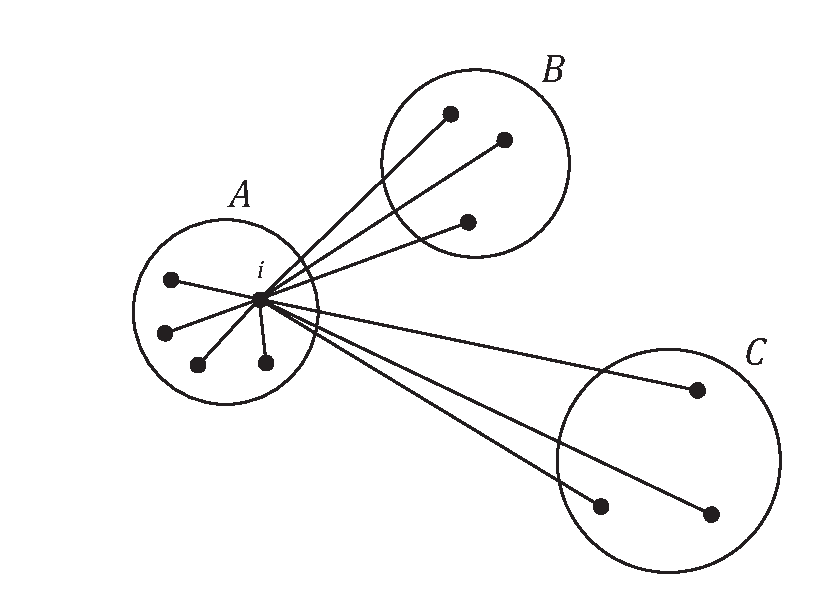
\includegraphics[width=0.5\textwidth]{images/silhouette_computation_clusters.pdf}
    \caption{Silhouette computation example for a single data point.
    \label{fig:silhouette-computation-clusters} }
\end{figure}

Therefore \citeauthor{silhouettes}, author of \citetitle{silhouettes}, speaks of detected clusters
as artificial or natural, based on visual inspection, and proceeds 
to introduce \emph{Silhouettes} as a graphical aid for detecting 
such artificial fusions of data. The silhouette of a data point is 
denoted by a numerical value in the interval $[-1, 1]$, denoting how well
the particular data point belongs to the cluster it is currently
assigned to. A higher value indicates a better assignment.

Silhouettes are, somewhat simplified, defined by dividing the mean
distance from the point of concern (in 
figure~\ref{fig:silhouette-computation-clusters} denoted by $i$) to
all other points in the same cluster $A$, with the mean distance from
$i$ to all points in the nearest not assigned cluster, $B$. The following
equation shows the computation process:
\begin{equation}
    \label{eq:silhouette-computation}
    s(i) = \frac{b(i) - a(i)}{\max\{a(i), b(i)\}}
\end{equation}
where $i$ is the point of concern, $a(i)$ is the average distance
from $i$ to all other points in $A$, and $b(i)$ is the average
distance from $i$ to all points in $B$.

Silhouettes were suggested to be visualized by a 
horizontal bar plot, each bar denoting the silhouette value of 
each point in the cluster the point was assigned to. 

Given that, it is desirable to have wide silhouettes describing the
clusters, and that the silhouettes should be even edged. A mean 
silhouette width $ \bar{s} $ can also be computed, in order of 
giving condensed, numerical interpretation of how natural the 
clustering is of a processed data set \cite{silhouettes}.

In a later work \citeauthor{finding-groups-in-data} suggests using
a \emph{Silhouette Coefficient} ($ SC $), that is the maximum 
$ \bar{s}(k) $ over various $ k $ using a partitioning clustering 
method
\begin{equation}
    \label{eq:silhouette_coefficient}
    SC = \max_{ k } \bar{s}(k)
\end{equation}
which suggests how well the data set is suitable for clustering 
given the particular clustering method being used.
Table \ref{table:silhouette-interpretation} provides a suggested
interpretation of the silhouette coefficient, as provided by
\citeauthor{finding-groups-in-data} \cite{finding-groups-in-data}.

\begin{table}
    \centering
    {\begin{tabular}{ | l | l | }
        \hline
        SC & Proposed interpretation \\
        \hline
        0.71 - 1.00 & A strong structure has been found.\\
        0.51 - 0.70 & A reasonable structure has been found.\\
        0.26 - 0.50 & The structure is weak and could be 
                      artificial.\\
        $<$    0.26 & No substantial structure has been found.\\
        \hline
    \end{tabular}}
    \caption{Silhouette Coefficient interpretation.} 
    \label{table:silhouette-interpretation}
\end{table}

If one considers table \ref{table:silhouette-interpretation} 
from a $ \bar{s} $ point of view instead of $ SC $, this should 
be applicable for determining the quality of found clusters by 
an arbitrary algorithm.

It is notable that silhouettes are not meaningful when clustering 
algorithms produce a single cluster, since the definition of a 
silhouette describes the relation of points similarity to its 
assigned cluster and the closest cluster which it is not assigned
to, which will not exist given that there is only one cluster. 
\citeauthor{silhouettes} suggests assigning this sort of
silhouette a value of 0 for comparison reasons, as this is the 
most neutral value. 

\subsection{Data Representation}
A sound way of representing detected clusters is necessary, in 
order not to have to re-run the clustering algorithms each 
time a knowledge discovery is requested. Being able to position 
clusters and use knowledge about previously recorded clusters is
another necessity, to make the algorithm learn based on user
corrections (of for instance the name of locations). 
After all, the sought result is to classify Moments
and clusters with \emph{semantically significant} and
\emph{meaningful} names, and 
being corrected by a user on a cluster name should trump 
everything else, thus being more significant. Detected clusters
at the same position as a previous should have the same name, not
only for being as correct as possible, but also in order 
not to be ambiguous in classified cluster names. 

Many databases today support geo-spatial queries for both points and
polygons\footnote{
    Here, only 2-dimensional data is considered which is the most 
    commonly supported, although support for 3-dimensial data exist
    in many database solutions.
}, and in this case it is the latter that is of interest. 
Being able to store clusters as areas, and persist these areas 
represented as polygons enable another level of detection for 
clusters, where it is possible to detect if it is a cluster that 
is known previously. Queries asking for overlapping clusters are
in general supported by 
\emph{Spatial Database Management Systems} (SDBMS) using 
\emph{Dimensionally Extended Nine-Intersection Model} 
DE-9IM\footnote{
    DE-9IM is a model for representing spatial relationships 
    between polygons and geo-spatial shapes. This is defined
    by a matrix specifying Interior, Boundary and Exterior 
    attributes between the different shapes, and varying 
    configuration of the resulting matrix is interpreted as
    spatial relationships such as \emph{Touches}, \emph{Disjoint},
    \emph{Equals} etc \cite{DE-9IM}. }

The support for performing geo-spatial queries on a database and 
doing this efficiently is usually implemented with some sort of 
\emph{spatial index}. Common implementations are R-trees 
and R*-trees, which fits the spatial entities into rectangles of
varying sizes in a tree structure, allowing a lookup time of 
\ordo{log(n)}, by balancing the trees \cite{R-trees, R*-trees}.

Apart from storing polygons, it is useful during this paper to
also persist the spatial points which make the cluster. This is 
for evaluation purposes, as algorithms examining the quality or
naturalness of a cluster in general needs access to all the points
in the particular cluster.

\subsubsection{RethinkDB}
RethinkDB will be used in the sought proof-of-concept implementation,
as it fulfills the necessary requirements, with support for spatial
queries and storage of spatial data both as geographical points, and
polygons.

It is an Open Source project hosted on GitHub, and has a growing 
community at the time of writing providing support when needed. Narrative
is currently using RethinkDB as a cache-layer for API requests, making
it an even stronger candidate for the proof-of-concept implementation.

\section{Classification}
Classification of data is closely related to clustering of data, 
and the two problems are not even distinguishable in all 
applications. 

\subsection{Bayesian Inference}

Bayesian inference is a methodology for updating beliefs about a model
when certain evidence is observed, while preserving some level of 
uncertainty.

The entry point is some \emph{Prior probability} $Pr(\theta)$ that the model 
we are observing is in world $\theta$. There exist \emph{likelihoods} 
$ Pr(x_i|\theta) $ that some \emph{evidence} $ x_i $ will be observed in
this $\theta$ world. Given this framework, the target is often to 
compute a \emph{Posterior probability} containing updated beliefs about
the state of the world provided the witnessed evidence. 

A model representing Bayesian beliefs can easily be graphically 
interpreted as a \emph{Bayesian Network}. Bayesian networks are Probability 
DAG:s (\emph{Directed Acyclic Graphs}), and are used for modeling the 
probability of certain events when other events are known. 

%% HERE

In this report, a Bayesian network is used to model the probability of a 
series of positions (or more exactly, photographs with positions attached)
enhanced with additional sensor data belonging to a certain class.

As this introduction previously established that expected results from 
clustering algorithm are not precisely defined and lies in the eyes of 
the beholder. If the results are somewhat fuzzy, and somehow can be 
computationally evaluated according to some metric, this should prove as 
a suitable parameter for an automatic decision algorithm, such as one 
powered by a Bayesian network, which is the idea behind the implementation
that is described. 

Bayesian networks are the base for Bayesian analysis, which starts with
a prior probability $ Pr(\theta) $ and a likelihood given $ Pr(x_i|\theta) $
in order to compute a posterior probability $ Pr(\theta|x_j) $. In the case
of this report, $ x_i $ represents some input probability while $ x_j $
represents some class or end condition.

With each inferred parameter, a dimension is added to the state-space\footnote{
    The state-space is defined as the possible states for a world to be in, and
    increases with each dimension added.
}. This makes high-dimensional models hard to observe and analyze by inspection, 
since modelling more then 3 or perhaps 4-dimensional probability space of 
various parameters is not possible to visualize. 

\subsubsection{Fitting of models}
As models become complex when inferring high dimensionality and observing
evidence (thus forcing other probabilities in the model to alter), 
visualization of the probability of a certain unobserved variable becomes
harder. Simply outputting some mathematical formula is not intuitively
graspable and computing such a formula is usually hard or impossible when other 
parameters have been described by sample data.
%and not by mathematical probability functions. 

\emph{Markov Chain Monte Carlo (MCMC)} are a category of algorithms 
dealing with this particular matter, and instead describes the probability
of theses parameters using thousands of samples. The main target is to 
cover as much of the state-space as possible by randomly drawing samples
in a manner that makes the returned collection as close to the true 
distribution as possible. 

When a fitting algorithm is proven to approach the true underlying 
distribution, when provided with enough steps and enough samples, it is 
denoted that the algorithm \emph{converges}. 

\subsubsection{PyMC}
\emph{PyMC} is the framework used for Bayesian modeling of the
classification problems in this report. PyMC:s online user manual
states:

\blockquote{
    ``PyMC is a python module that implements Bayesian statistical 
    models and fitting algorithms, including Markov chain Monte Carlo. 
    Its flexibility and extensibility make it applicable to a large 
    suite of problems. Along with core sampling functionality, 
    PyMC includes methods for summarizing output, plotting, 
    goodness-of-fit and convergence diagnostics.''
    - PyMC User's Manual \cite{pymc}.}

PyMC fits the needs of this project well, as it implements the
core functionality necessary for Bayesian inference such as a range
of probability functions as well as fitting algorithms, mainly MCMC.
%(in particular, a flavor of MCMC called INSERT HERE)
It is also 
bundled with algorithms for finding an appropriate starting point for
the fitting algorithms to work with, as this affects the rate of 
convergence for the fitting algorithm.

\section{Limitations}

\subsection{Image analysis}
Only very simple and limited image analysis is applied in this 
report, as this could easily have made subject for a thesis of 
its own (as is the case with other reports) 
\cite{content-based-classification, framework-classification}. 

The purpose of this thesis is not classification of images as
such, but of small series of data samples of varying length. 

\subsection{Individual classification}
Interesting as it might be with performing individual 
classification of data, in this case images, this is deemed
outside of scope for this report, due to time limitations. 

The subject considered is, as mentioned above, deducting 
information about a data set as a whole given attributes in 
separate data.

\subsection{Automatic Learning of Network structure}
In machine learning there exist a lot of literature about the
subject of automatically determining network structure of 
a Bayesian network, opposed to let it be specified by an
expert. The intent is here to describe the automated process
of data set classification, and the initial step such as 
setting up the decision network is assumed to be done. For 
simplicity reasons, the second approach is chosen, and 
extending the work later on by learning the network structure
computationally does not interfere with the work of this 
report.

\subsection{Exact Probabilities}
Exact distributions of probabilities of events are hard to 
come by, and are by its nature virtually impossible to 
confirm (given that it is probabilities). This report will not
focus on determining these optimally, but rather leave the 
estimated distributions to be decided based on a bit of logical
reasoning. 

\subsection{Semantic Significance}
Choosing labels for derived classes is a problem of its own, and
will not to its full extent be discussed in this report. As 
\citeauthor{content-based-classification}, authors of 
papers~\citetitle{framework-classification} 
and~\citetitle{content-based-classification},
% Would like to reference both, but it is the same author, 
% "framework-classification"
mentions, search queries often describe more high-level attributes
about data sets, or images in this case, such as a search would more
likely consist of the word "sunrise" when looking for an image, than
"predominantly red and orange" 
\cite{framework-classification, content-based-classification}.

The semantic significance of the label of a class can therefore 
describe how meaningful that label is, although assessing in full 
scale how significant the labels are in this report will be left 
for future research.
\subsection{Only 2-dimensional spatial data is considered}
One might consider data of higher dimensionality, encountering
other problems than the spatial clustering in this thesis report.
This will however not be done here, as this does not seem to
have enough relevance for this case. 

\section{Related Work}
\citetitle{finding-groups-in-data} by 
\citeauthor{finding-groups-in-data} is regarded by many as the 
classic text-book in cluster analysis which provides and 
introduces several theories that prove the foundation of 
cluster theory today \cite{finding-groups-in-data}.
\citeauthor{silhouettes} is also the author of the 
paper~\cite{silhouettes}, that introduces a universal way of 
evaluating clustering performance under certain conditions, such 
as that the number of clusters has to be greater than 1. This 
method is used in this thesis and is discussed itself, based on 
its suitability to accommodate for different clustering solutions.

Article~\cite{why-so-many-clustering-algorithms} is a position 
paper describing ways of looking at clusters and cluster analysis 
on a broad spectrum, and explains the difficulties as well as 
why there is no universal solution to clustering. 

The papers~\cite{DBSCAN, OPTICS, CLARANS, Ejcluster, SLINK, clusterpath, k-means, finding-groups-in-data} 
all describe various clustering algorithms used and were considered 
as prospects for evaluation in this thesis. 

Papers~\cite{R-trees, R*-trees} both describe ways of implementing 
spatial indexes, which are the core of a spatial data base and making 
spatial queries possible in an efficient manner. 

The article~\citetitle{P-DBSCAN} at first glance seem to be very similar in 
its aim as this this, but the difference lies in intention. While 
\citeauthor{P-DBSCAN} tries to deduct information about attractive
areas and places using clustering of photographs, the approach of this 
paper is to deduct information about a series of photos using areas 
and places. \cite{P-DBSCAN}

The paper~\cite{bayesian-class-gauss-proc} introduces learning of detection of 
probabilities modeled by Gaussian Processes by interpreting the 
classification as a regression problem. This allows small training 
sets, which Bayesian numerical techniques for calculating the trace 
and determinant was not as tolerant of. 

Papers~\cite{content-based-classification, framework-classification} use a
Bayesian approach for classifying individual images based on their 
visual attributes, which is fairly closely related to this work. This
provides interesting results inspiring this thesis, with the difference
of classifying series of images instead of single images, and choosing
other attributes to base the classification on.

\cite{bayesian-methods-for-hackers} explains thoroughly how one might
regard Bayesian inference and methods from a programming perspective 
with examples in PyMC, rather than using traditional mathematical notation
to address the problems. 
(Not clear if this is a valid resource, but it sure was helpful).
Similarly, \cite{bayesian-theory} provides more in-depth foundation
with weight distributed on the theoretical parts of Bayesian 
analysis.

\cite{the-most-dangerous-equation} explains the pitfalls of de Moivres 
equation by reciting some statistical mishaps throughout history. This 
explains the care one has to take to not draw premature conclusions from
small data sets. 

% Re-read
\cite{discovering-moving-clusters} describes discovery moving of spatial 
clusters, and thus introduces another dimension into the clustering; time.
This is similar to the approach suggested in this thesis, with the 
difference of observing a lot of spatial points at once. 

\cite{hierarchical-evaluation} discusses and compares different 
methods of evaluation hierarchical clustering algorithms. 

\cite{twitter-geo} is an example of a real-time, big data application 
using spatial content in the social network Twitter to locate events
on a map, similar

Article~\cite{iphone-wifi} evaluates the accurateness of mobile units 
with regard to GPS data, and different techniques that can be used for 
obtaining this in an urban area. This is useful to keep in mind, as 
a similar implementation for life-logging devices and the Clip lies 
close in the future.

\section{Report Structure}

This section has presented the motivation and technical foundation
for the work done in this paper. More specific implementation 
details and theory will be addressed in chapter \ref{ch:method}.
The results of these implementations will be presented with 
measured test data in chapter \ref{ch:result}. These results 
will later be evaluated and discussed under chapter 
\ref{ch:discussion}, as well as other factors that might have 
influenced the results. Finally, a conclusion is drawn in chapter 
\ref{ch:conclusion} as well as suggestions for further research 
on the subject.

The appendices contain further implementation details beyond what
is described in the report. These should not be necessary to grasp
the main outlines of the report, but prove interesting for a full
understanding of how algorithms have been implemented in this work.

\chapter{Method}
\label{ch:method}
\section{Classification}
The classification is the main target for the proof-of-concept 
implementation, described below. 

The main targets for the classification algorithm is determined by some 
spatial clustering algorithm. This data set might either be entire 
Moments if no cluster is found, or if the entire data set is regarded to
be a cluster. If several clusters are found, these will be classified 
individually. Moments or clusters sent to the classification algorithm 
will below be referenced to as an activity (not to be confused with the
later mentioned class \emph{activity}, representing the amount of
physical activity).

\subsection{Input Beliefs - Evidence}
%%%%%%%%%%%%%%%%%%%%%%%%%%%%%%%%%%%%%%%%%%%% 80 line marker %%%%%%%%%%%%%%%
In order to establish a prior belief in the data to model, it is 
necessary to model the estimated prior distribution of the input data to 
model the prior belief in class assignment. This is later updated based on 
observations of the data, and beliefs are reinforced or skewed based on 
these observations into \emph{posterior beliefs}.

\subsubsection{Accelerometer}
The accelerometer provides 3 values for each sample taken by the sensor, 
one for each direction in the three dimensional coordinate system. As the 
Clip can be mounted on the user in different ways, as well as being tilted, 
these acceleration vectors are not bound to some specific orientation in
relation with the earths coordinate system.

Most commonly the Clip is either fitted on the user with the buckle facing
down, or horizontally (either left or right). This makes the x-axis and
y-axis interchangeable.

\begin{figure}[ht]
    \centering
    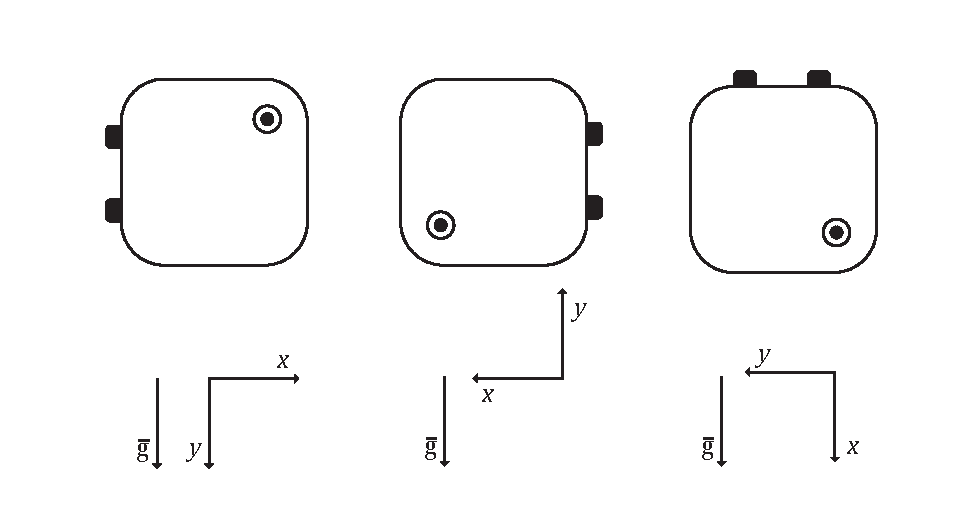
\includegraphics[width=0.7\textwidth]{images/narrative_clip_orientation.pdf}
    \caption{ An illustration of the most plausible orientations of The Clip as 
        worn by the user. \label{fig:narrative-clip-orientation} }
\end{figure}

Given the uncertainty of which direction the sample was recorded in, the
solution would be to use the magnitude of the vectors combined, and 
ignore the direction of the resulting vector\footnote{
    If the Clips orientation was of interest, or there was a specific need
    to know each composant of the accelerometer vector, it could be assumed
    that the composant being closest to $ g \approx 9.8 m/s^2 $ in magnitude was 
    the direction facing downward. The user is not likely to change the 
    orientation of the Clip between each photo, so detecting the orientation
    based on multiple photos seems more robust and feasible. 
}. Chances that the combined
vectors should sum up to the original, stationary vector when moving seem
slim. 

An accelerometer measures \emph{proper acceleration}\footnote{
    Proper acceleration is the physical acceleration that is experienced 
    by an object, including gravitational force. }
and will therefore usually have a constant approximated value corresponding 
to $ g \approx 9.8 m/s^2 $ when stationary, and somewhere around that value when
a user is in motion. 

The most feasible application of the accelerometer seems to be determining
the level of activity in the Moment. When a user is active (such as being
out for a run or sporting), it is probable that the acceleration is varying, 
partly because of the actual movement, and partly because the Clip jiggles 
around when in movement. 

Given the above, the most feasible distribution of the samples observed
seem to be around $g$, with decreasing probability around this point as
the acceleration diverges more and more from $g$. Such a distribution
could be described using a 
\emph{Normal distribution} with the following \emph{probability density 
function}:
\begin{definition}[Normal Distribution Probability Density Function]
\label{definition:normal-pdf}
$$
    PDF_{Norm}(x, \mu, \sigma) = 
        \frac{1}{\sigma \sqrt{2\pi} } 
                 e^{ -\frac{(x-\mu)^2}{2\sigma^2} }
$$
\end{definition}

We denote a stochastic variable that is Normally distributed by
\begin{definition}[Normally distributed variable]
\label{definition:normal-variable}
$$
    X_i \sim Norm(\mu, \sigma)
$$
\end{definition}
where $\mu$ is the expected mean value (which we expect to be $g \approx 9.8 m/s^2$
or equivalent), and $\sigma$ the standard deviation.

In order to measure how the acceleration varies, the 
\emph{auto-correlation} (or serial correlation) of the samples can be used. The 
auto-correlation is defined as the cross-correlation of a series of 
samples with itself. This is generally used in statistics as a measurement of 
the predictability of a series of samples from a distribution, and predicts 
how much a value is likely to change given two consecutive measurements. 

This is another reason to use the magnitude of the accelerometer vector, as
values close to 0 (as the y- and z-axis tend to be while stationary) show 
very little auto-correlation, due to small changes in small values.

\subsubsection{Area}
The area size of an activity. When there are no spatial data points
available for an activity, this is for simplicity reasons assumed to 
be $0$, indicating that a user is in such a small area that it can be
neglected. 
\begin{definition}[Area distribution]
\label{definition:area-variable}
$$
    X_{area} \sim Norm(\mu_{area}, \sigma_{area})
$$
\end{definition}
where $\mu_{area}$ is found by using the mean area value in a subset of 
all currently sampled activities, and $\sigma$ is the variance in the same 
data set.  

\subsubsection{Face Detection}
Narrative runs a face detection algorithm on the set of their images, 
determining whether any face is present or not in a photo. The ratio 
between images with faces and without are of particular interest, as we can 
see below, and is deduced for each activity in the classification algorithm. 
The faces/photos distribution is modelled as 
\begin{definition}[Faces/Photos distribution]
\label{definition:faces-variable}
$$
    X_{faces} \sim Norm(\mu_{faces}, \sigma_{faces})
$$
\end{definition}
where $\mu$ is found by using the mean value in a subset of all currently 
stored activities, and $\sigma$ is the variance in the same data set.  

\subsubsection{Time}
The starting time of a Moment is probably more likely to occur mid-day or 
during the evening, when more special activities occur and the users decide 
to clip it on. This timely information is used to detect where users are 
spending their time, and if their activity is work-related or recreational, 
on their spare time. The probability of observing such a timestamp is therefor 
estimated using a \emph{Binomial Distribution}, with the following
\emph{probability mass function}\footnote{
    This is denoted \emph{probability mass function} instead of the 
    previously mentioned \emph{probability density function}. This is 
    essentially the same thing, with the difference of the first being
    a continuous distribution while the latter is discrete. }:
\begin{definition}[Binomial Distribution Probability Mass Function]
\label{definition:binomial-pmf}
$$
    PMF_{Bin}(k;n, p) = \Pr(X = k) = {n\choose k}p^k(1-p)^{n-k}
$$
\end{definition}

We denote a stochastic variable that is Binomially distributed by
\begin{definition}[Binomially distributed variable]
\label{definition:binomial-variable}
$$
    X_i \sim Bin(n, p)
$$
\end{definition}
where $n$ is the number of trials attempted and $p$ is the expected
number of successes.

\subsection{Output Beliefs}
The target is to classify a received data set into a finite set of classes. 
According to Bayesian methodology, it is necessary to model an experts 
belief in the distribution of assigned classes. First of all, assume that 
an input data set can never partly be assigned a class but always fully. 
The assignment is either done, or not. This model was described by the 
Swiss mathematician Jakob Bernoulli, who coined the 
\emph{Bernoulli distribution} with the following probability mass function:
\begin{definition}[Bernoulli Probability Mass Function]
\label{definition:bernoulli-pmf}
$$
    PMF_{Bernoulli}(k,p) =
    \begin{cases} 
        p   & \mathrm{if} \; k = 1 \\
        1-p & \mathrm{if} \; k = 0 \\
    \end{cases}
$$
\end{definition}
This describes the probability $p$ of a class being assigned to the data 
set received. We denote a stochastic variable that is Bernoulli 
distributed, the prior probability of a class $i$ being assigned, by
\begin{definition}[Bernoulli distributed variable]
\label{definition:bernoulli-variable}
$$
    X_i \sim Ber(p_i)
$$
\end{definition}

This prior probability is modelled by one or several threshold values,
which determine the probability of which class is used. 

The inferred classes that we will attempt to predict are the following:
\begin{itemize}
    \item \emph{Social} - Whether the user is engaging in a social 
        activity or not. This is believed to be effected by the amount
        of faces in the photos in a series. 
    \item \emph{Working} - The users working status during a Moment. 
        This is believed to be affected by the starting point of the 
        series of images, as well as the area size of the detected
        clusters. 
    \item \emph{Indoors} - Whether the user is indoors or not. This is 
        believed to be affected by the area size of an activity.
    \item \emph{Movement} - How much physical activity the user is 
        undergoing during an activity. This is 
        believed to be affected by the auto-correlations mean value 
        of an activity.
\end{itemize}

These classes can take on two discrete values; either they are assigned
or not (this is somewhat simplified with the labels for the classes - 
with friends or not alone, for \emph{Social}, working or off hours
for \emph{Working} and indoors or outdoors for \emph{Indoors}). Thus, 
these are Bernoulli distributed as mentioned above:
\begin{equation}
    \label{eq:bernoulli-classification}
    \begin{split}
        X_{social}  &\sim Ber(p_{social})  \\
        X_{indoors} &\sim Ber(p_{indoors}) \\
        X_{working} &\sim Ber(p_{working}) 
    \end{split}
\end{equation}
where $p_i$ depends on the parent values (see 
figure~\ref{fig:bayes-network} on page~\pageref{fig:bayes-network}).

The exception here is $X_{activity}$ which is 
\emph{Categorically distributed}, a generalization of the Bernoulli
distribution:
\begin{definition}[Categorical Probability Mass Function]
\label{definition:categorical-pmf}
$$
    PMF_{Categorical}(k,p) = p_i
$$
\end{definition}
where $p_i$ represents the probability case $i$ to be true. 
We denote a stochastic variable that is Categorically 
distributed, the prior probability of a class $i$ being assigned, by
\begin{definition}[Categorically distributed variable]
\label{definition:categorical-variable}
$$
    X_i \sim Cat(p_1, ..., p_i)
$$
\end{definition}

It is worth reminding here that it is the concept of using Bayesian 
Inference as a classification tool for life-logging environments that 
is up for testing, and not necessarily the model for each 
implementation. As mentioned among the limitations, the structure of
the network is assumed to be fixed from the start and automated learning
of the structure is not applicable. 
Because of this, it seems more suitable to infer a rather 
simple and shallow model to test the concept. Using several classes
that only depend on a few parameters allow some error and redundancy 
to sneak in due to model construction errors, which will be discussed 
later in this thesis.  

\subsection{Model Parameters}
All parameters mentioned above can be observed by inspecting data, and 
are thus the evidence $E$ that can be observed when the model is in certain 
world state. Modelling these correctly is nevertheless important anyway, in 
the case of missing values. 

The classification depends on a series of model parameters, such as thresholds
for when different classes should be inferred. 

These breakpoints are be denoted as model parameters, and are of interest for
learning how classification can be done. While approximating these with a 
well-formed probability function is a cause for faster convergence and faster
learning, it is essential that all possibilities are covered. If the model 
parameter is not covered by it's initial probabilities, the model is not 
correct and will probably not provide the desired results. 

These model parameters will for simplicity's sake be universal in this master
thesis, but should probably later on be possible to tweak for each individual, 
with the aid of a learned starting point.

\subsubsection{Learning the parameters}
In order to make our hypothesis as credible as possible given previously 
recorded classifications made by human observation, the thresholds need to
be properly set. This is done by letting both our samples of the observed
data of several Moments be fixed, as well as the classification that later
is to be determined for other activities. The only thing that is then allowed
to vary in order to make the model true, is the thresholds, our hypothesis, 
forcing these variables to take on relevant values. 

By doing this for a decent amount of pre-determined classifications, 
and letting MCMC in PyMC fit the model by drawing thousands of samples of this 
distribution, by randomly walking over the set, something very close to the 
true distribution is learned, that can be used as the hypothesis in future 
classifications. 

In this instance, a rather small sample is used, yielding a hypothesis 
in danger of being biased. In a real-world application, this sample of
classification would be much bigger, but this sample size of ~50 classifications
should suffice to prove the concept. 

\subsection{The Bayesian Network}
The dependencies between various stochastic variables can be made more 
over-viewable when represented graphically as a network, see 
figure~\ref{fig:bayes-network}. In this figure, the top ellipsoids with a solid 
border marks the evidence $E$ observed for each activity. The squares are the 
thresholds, or model parameters that have been learnt via Bayesian inference
and fitting the model with pre-classified data. This is our hypothesis. 
The circles with a dashed border is the classes of which we try to determine 
our posterior belief after observing the evidence.

\begin{figure}[ht]
    \centering
    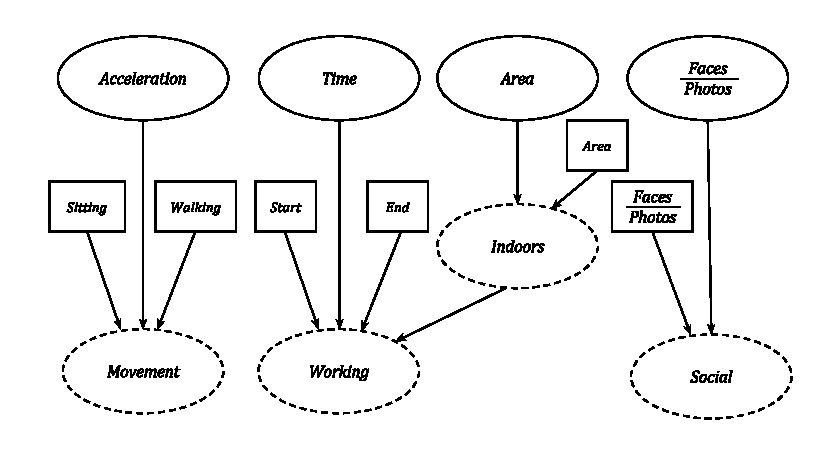
\includegraphics[width=0.8\textwidth]{images/bayes_network.pdf}
    \caption{A graphical view of the bayesian network modelled for deriving the
        classes. \label{fig:bayes-network} }
\end{figure}

\subsection{Curse of Dimensionality}
The \emph{curse of dimensionality} is a problem that arises in cluster 
analysis and data mining applications where a lot of dimensions or 
considered features in the regarded data causes data that are fairly 
similar to appear to be very dissimilar due a few to outlying, less 
important property values. 

This problem arises when the observed data contains a lot of parameters that 
can take on very different values.

In this work, this is mainly a problem in the inference domain and not in the 
spatial clustering domain, as spatial data in 
it's nature is two-dimensional (at least in this case, as the earths
surface can be regarded as two-dimensional, from a geographical point of 
view).

This is why clustering of spatial points precedes the Bayesian inference 
in this work, in order of decreasing the dimensionality and learning 
something useful from the spatial data before moving on to tackle other 
quantifiable data: as for each comparable spatial point in the data set, we 
would need to model some sort of random variable, mapping against one 
dimension. This could easily sum up to several hundreds of dimensions, in 
the spatial analysis alone! Clustering algorithms exist in Bayesian 
notations as well, and one might even attempt to formulate the ones 
mentioned in this report in a more statistical-oriented fashion, but the 
main advantage here is to decrease the number of dimensions for further 
analysis in several steps. A pitfall to watch out for with this approach 
is removing more information than necessary, and thus making a biased 
analysis at a later stage due to unintentional biased information loss.

\subsection{Evaluating the Classification}
The proof-of-concept implementation will double as an evaluation program
visualizing users Moments and providing the deducted classifications, and
at the same time receive feedback from the users.

This is implemented as a browser extension, adding content to Narratives
web application and allows users to get classifications provided by the 
Bayesian inference framework set up for their own Moments. This as no one 
knows better how to classify an activity than the user who performed it, 
and therefore no one should be better at evaluating the algorithm 
performing classifications on it. 

Firstly, the users are presented with the option to run the classification
algorithm on a Moment (as they might choose not to provide every Moment
for the study for privacy purposes). When choosing to classify, a
visually comprehensive overview of their images and whereabouts during
this Moment is presented to them, as well as a classification of the 
activity or activities. After this, the users are provided with a form
where they evaluate the classifications quality on a 5-step scale, as
well as perform the same classification as the algorithm did. A comment
field is also present for commenting on the classification performance. 

In this scenario, in order to evaluate the algorithms performance, the 
users classifications is regarded as the truth. Some error can of course
be introduced in the form of users misinterpreting class definitions, but
this will be assumed to be an negligible amount of error.

Weighed into this is also the amount of false positives and false negatives
encountered. A false positive is considered to be a wrongful classification
where a \emph{semantically charged} class is chosen over a more neutral class, 
whereas a false negative denotes the opposite. These semantically charged
classes consists of the a set of classes that would actually be visible to 
the end user in a real implementation, since these denotes that something 
special happening in an activity, and considered more interesting than the
alternative. An example of this being that the social label 
\emph{With Friends} is probably more interesting and attractive to the user 
than the alternative \emph{Alone}. A false positive would in this case 
be for an algorithm to select a label \emph{With Friends} for a users
activity when the user actually was alone. 

\section{Clustering}

Three algorithms are chosen for evaluating various algorithms for clustering, 
each being a representative from the traditional breakdown of clustering 
algorithm types\footnote{
    For a more precise overview of these algorithms than provided in the
    previous chapter, please see 
    appendix~\ref{app:clustering-algorithms-theory}. }:
\begin{itemize}
    \item CLARANS
    \item DBSCAN
    \item SLINK
\end{itemize}

Because clustering algorithms differ very much, both in execution but also in 
output, these will be assessed in slightly different ways. The algorithms are
tested on the same data sets and output will be compared both by using 
silhouettes and run-time, but also evaluated by the extra features that each 
algorithm bring. In the end, the suitability for this particular task of 
detecting clusters in data sets on the move is evaluated, and anything an 
algorithm can provide as an advantage will be taken into account. The results
of the silhouettes and run-time will be presented in the following chapter,
while the latter discussion of further algorithm advantages will be discussed
in the discussion chapter. 

\subsection{Clustering parameters}
When using clustering algorithms, the cluster parameters are important tools 
for describing what type of clusters that are desired. Therefore, some 
guidelines are introduced as to how the cluster parameters are set when 
evaluating the cluster performance of the algorithms.

\subsubsection{CLARANS}
CLARANS runs several times over the data set, with different $k$. Inspection
shows that these data sets seldom contains more than a few clusters, so therefore
$k$ will go from 1 to 5 in order of finding a suitable $k_{nat}$\footnote{
    In the original report, CLARANS is meant to throw away clusters producing
    clusters with no significant structure found. This is its way of disregarding
    noise. It is not done in this thesis, as for potential detection of 
    activities, these clusters would be used as travels from one activity to
    another. }.

As for $num\_local$ and $max\_neighbour$, these need to be large enough that
it is likely that a good solution is found. Setting these to $10\%$ and 
$20\%$ of the desired data set respectively, seems to lead to consistent results. 

\subsubsection{DBSCAN}
A main upside of DBSCAN is its ability to discard points as noise, 
which proves useful in this particular case where combinations of 
clusters and paths exists, and paths can be discarded by tweaking 
the clustering parameters $ \epsilon $ and $ minPts $. This is the case
when we want to discard paths for instance walking speed, $ v_{walking} $
if we choose  $ \epsilon $ and $ minPts $ as 
\begin{equation}
    \label{eq:minPts_eps_condition}
    minPts \times v_{walking} \times 30 < \epsilon - C_{margin}
\end{equation}
with some safety margin constant $ C_{margin} $. This condition is 
illustrated in figure~\ref{fig:epsilon_minpts_condition}.

\begin{figure}[ht]
    \centering
    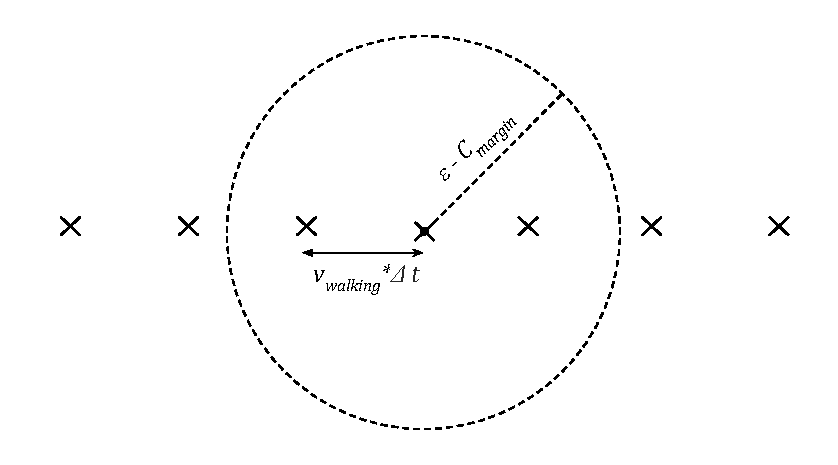
\includegraphics[width=0.5\textwidth]{images/epsilon_minpts_condition.pdf}
    \caption{ An illustration of the condition for choosing $ \epsilon $ and 
              $ minPts $ to exclude paths. \label{fig:epsilon_minpts_condition} }
\end{figure}

In order of keeping clusters significant enough, we let $minPts$ be
$10\%$ of the size of the data set, and set $C_{margin}$ to 
$minPts \times v_{walking} \times 15$, and let $\epsilon$ take
on the smallest value possible while still fulfilling 
equation~\ref{eq:minPts_eps_condition}.

\subsubsection{SLINK}
SLINK's cutoff function will consist of a distance cutoff condition same as 
DBSCAN's $ \epsilon $. 

\subsection{Detected Clusters}
A frequent scenario for using the Clip is when the user puts it on, then 
carries around for a long period of time at several locations, experiencing 
different activities. Deduction of qualitative information from life-logging 
experiences revolve partially around distinguishing these activities from 
each other, and this is where spatial clustering comes in handy. In this 
particular instance, a form of clustering has already been done, partitioning
long series of images into Moments using timestamps and RGB-cubes from photos
to detect the start of a new Moment. 

Therefore it is preferable to run the proposed spatial clustering algorithms
earlier in the pipeline than the proof-of-concept implementation in this paper
suggests, and this is why these algorithms will be tested on data sets not
only consisting of said Moments. But, as stated above, the proof-of-concept
implementation will only contain spatial clustering on a Moment-level. This 
will be provided by DBSCAN, as it is better suited for small data-sets where
only one cluster is found, or none at all for that matter. The algorithm
comparison however, will run on bigger data sets. 

A distinction between when a cluster has been detected and not has to be made 
as well, as the absence of a cluster can be interpreted as a user travelling 
between two sites.

\subsection{Assessed Spatial Data Sets}
The data sets on which the algorithms performance is assessed are real-world
spatial GPS data from users, chosen in a representative manner. The sets 
displayed in this report do not contain any map background, in order to
preserve anonymity.

These data sets consist both of data already divided into Moments, and 
longer data series merged together, providing more quantitative clustering
possibilities, and more possible clusters. 

\section{Big Data Ethics}
Given the current development of the technology revolving around Big Data
and deducting user behaviour given statistical information where the privacy 
of the end users needs to be discussed. Current literature and articles are
evaluated to get an overview of the current status of the debate, with 
the focus of life-logging devices as company services. 


\chapter{Result}
\label{ch:result}
\section{Clustering}
\emph{Most of the figures presented in this section are also available in 
appendix~\ref{app:larger-figures} as larger versions.}

\subsection{Small Data Set Activity Detection}
This section addresses data sets consisting of $822$ Moments, ranging 
from a few data points to thousands in each set. All three algorithms
have been given an attempt to cluster each Moment. The
\emph{haversine}\footnote{
    The haversine function, also called the great circle distance, 
    takes the curvature of the earth in consideration when measuring long
    distances between latitudes and longitudes \cite{haversine}.
} method is used for distance measurements. A computation is aborted if 
it takes longer than $100$ seconds, as the clustering is intended to be 
done automatically and in real-time\footnote{
    This is implied by the server-side placement of the clustering algorithm, and the intention to automate the process. For an automated service in the
    cloud with many users, the cost of CPU computations are not feasible
    if a service such as this takes more than a few seconds. 
}, where a run-time of close to a minute is not feasible. Results are 
excluded from a algorithms computation result set if it did not finish 
in time. In total, CLARANS timed out on $43$ of the Moments, and 
DBSCAN and SLINK did the same with $1$ each.

\subsubsection{Performance}

\begin{figure}[ht!]
    \centering
    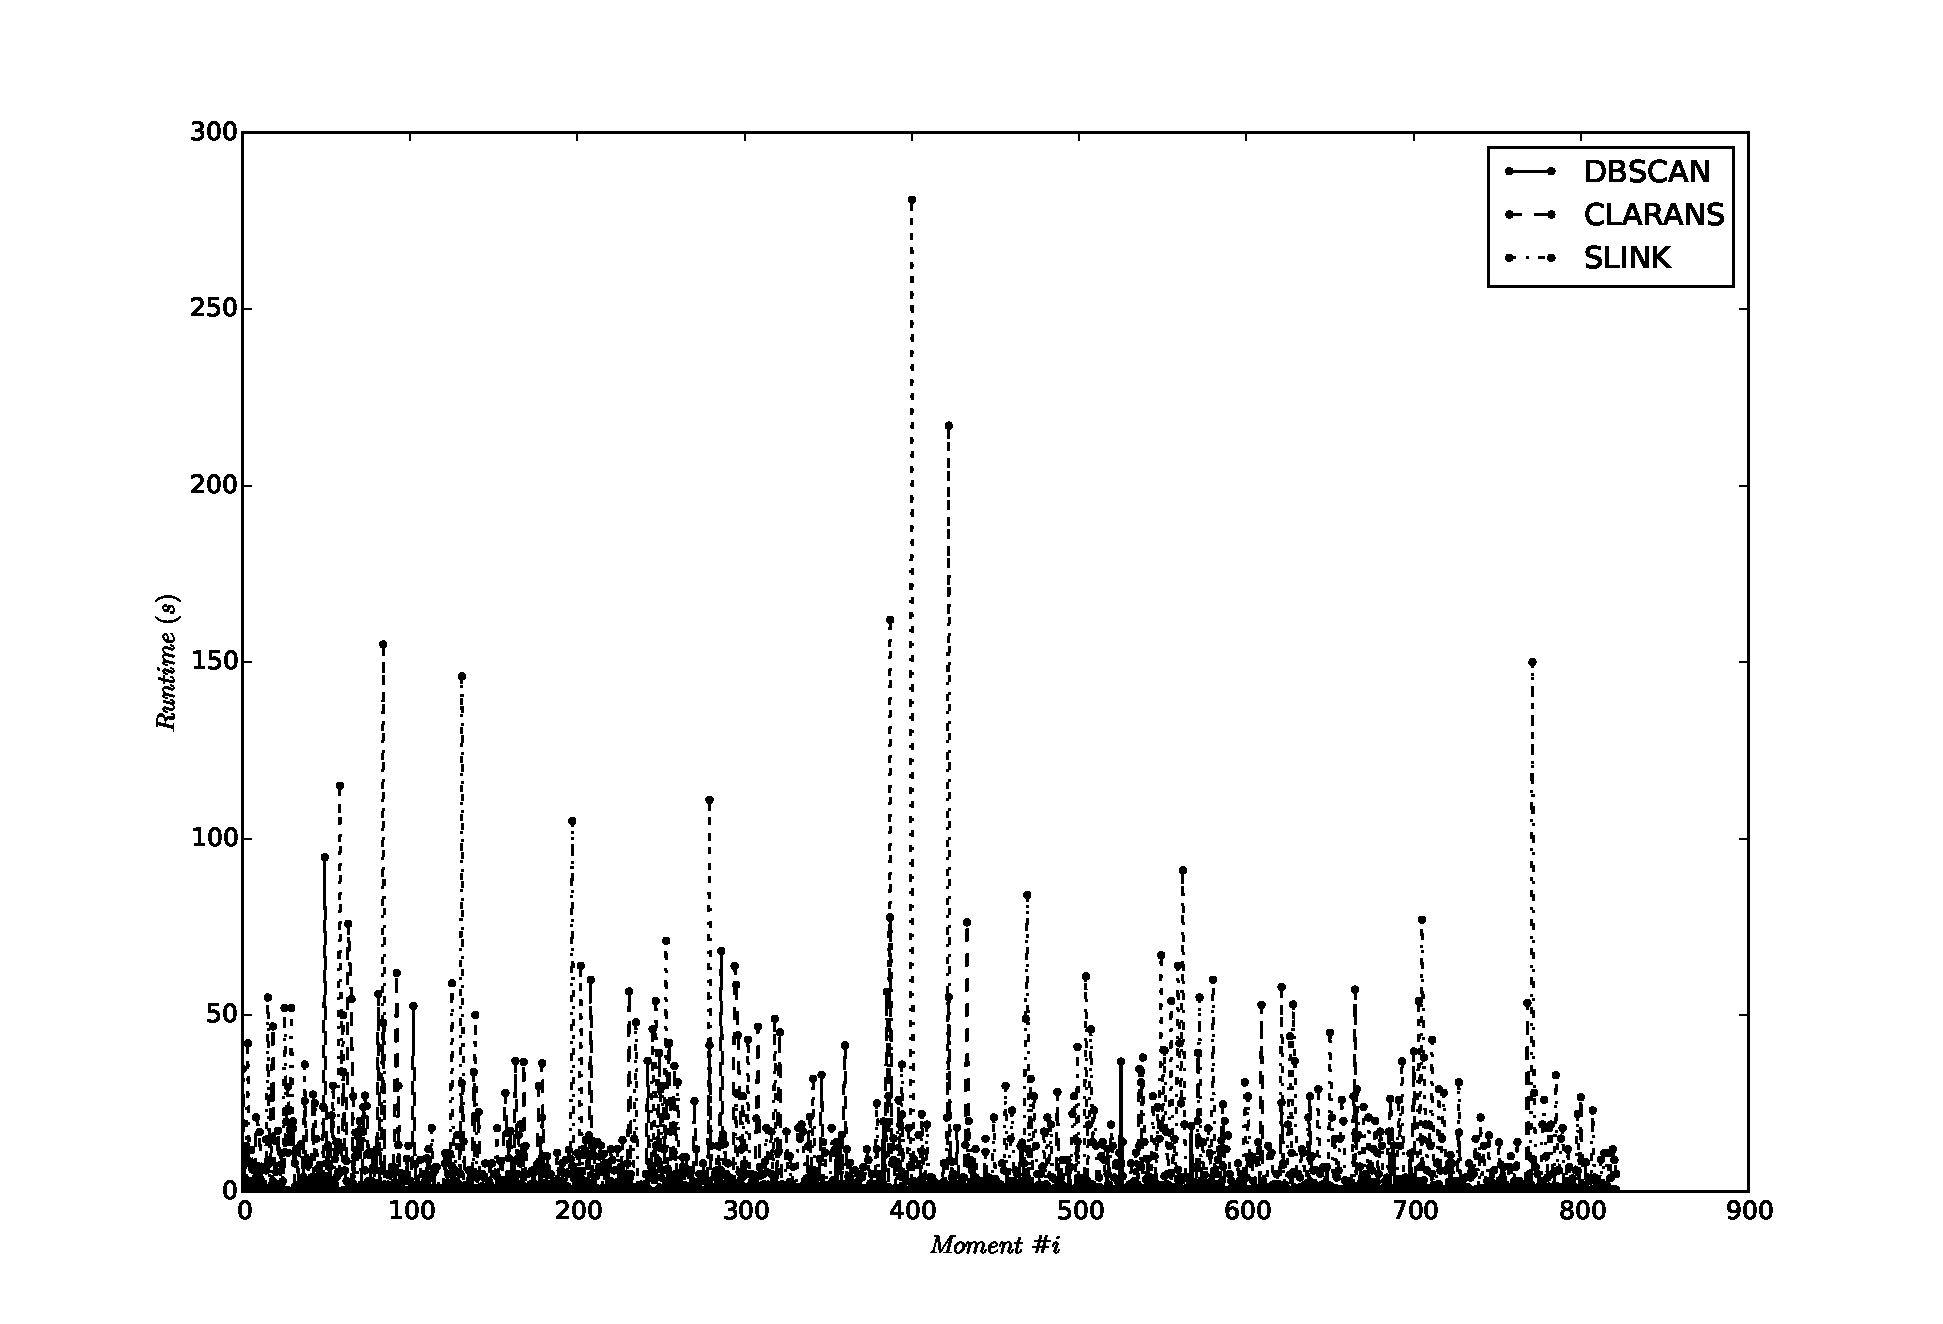
\includegraphics[width=0.9\textwidth]{plots/moment_runtime_plot.pdf}
    \caption{Run-time for clustering algorithms over Moments.
    \label{fig:moment-runtime-plot} }
\end{figure}

%%%%%%%%%%%%%%%%%%%%%%%%%%%%%%%%%%%%%%%%%%%% 80 line marker %%%%%%%%%%%%%%%
To evaluate the efficiency of the algorithms, the run-time for 
each algorithm over various Moments is plotted. 
Figure~\ref{fig:moment-runtime-plot} provides an overview over the run-time 
on Moments ordered randomly\footnote{
    The Moments in this plot is actually ordered by an internal Moment ID 
    provided by the database, although this is not of importance in this 
    section. For all intents and purposes, these are randomly ordered.
}. 
 
\begin{figure}[ht]
    \centering
    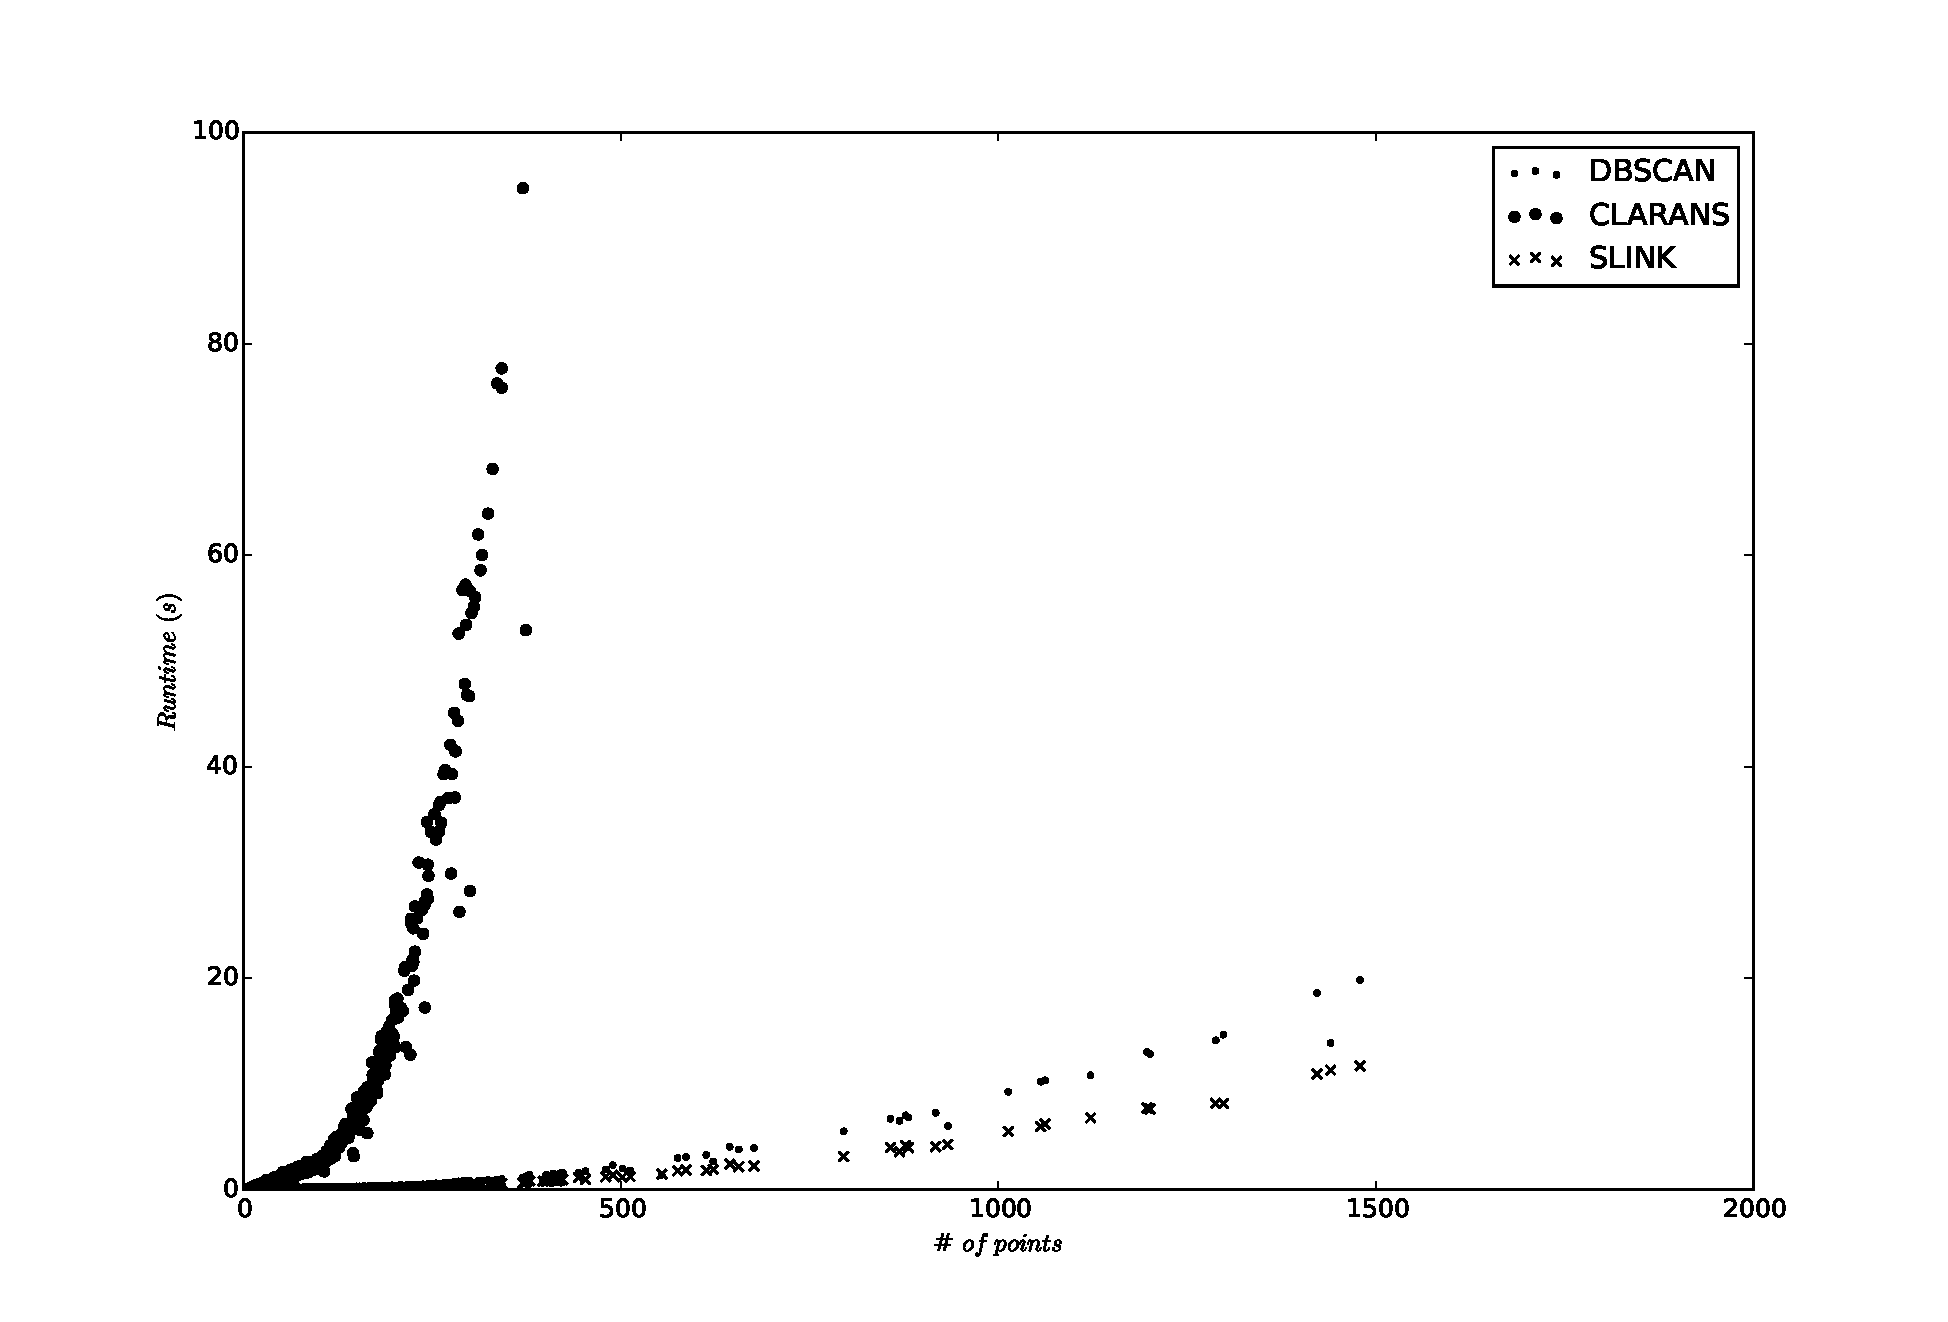
\includegraphics[width=0.9\textwidth]{plots/moment_runtime_scatter.pdf}
    \caption{Run-time for clustering algorithms over Moments, by number of
        points in the Moment.
    \label{fig:moment-runtime-scatter} }
\end{figure}

A more intuitive view is provided by figure~\ref{fig:moment-runtime-scatter}, 
where the run time of each point is mapped with the number of points in each 
Moment. This obviously provides a hint towards the time-complexity of each 
algorithm, which becomes quite clear. 

\cleartoleftpage

\subsubsection{Silhouettes}

\begin{figure}[ht]
    \centering
    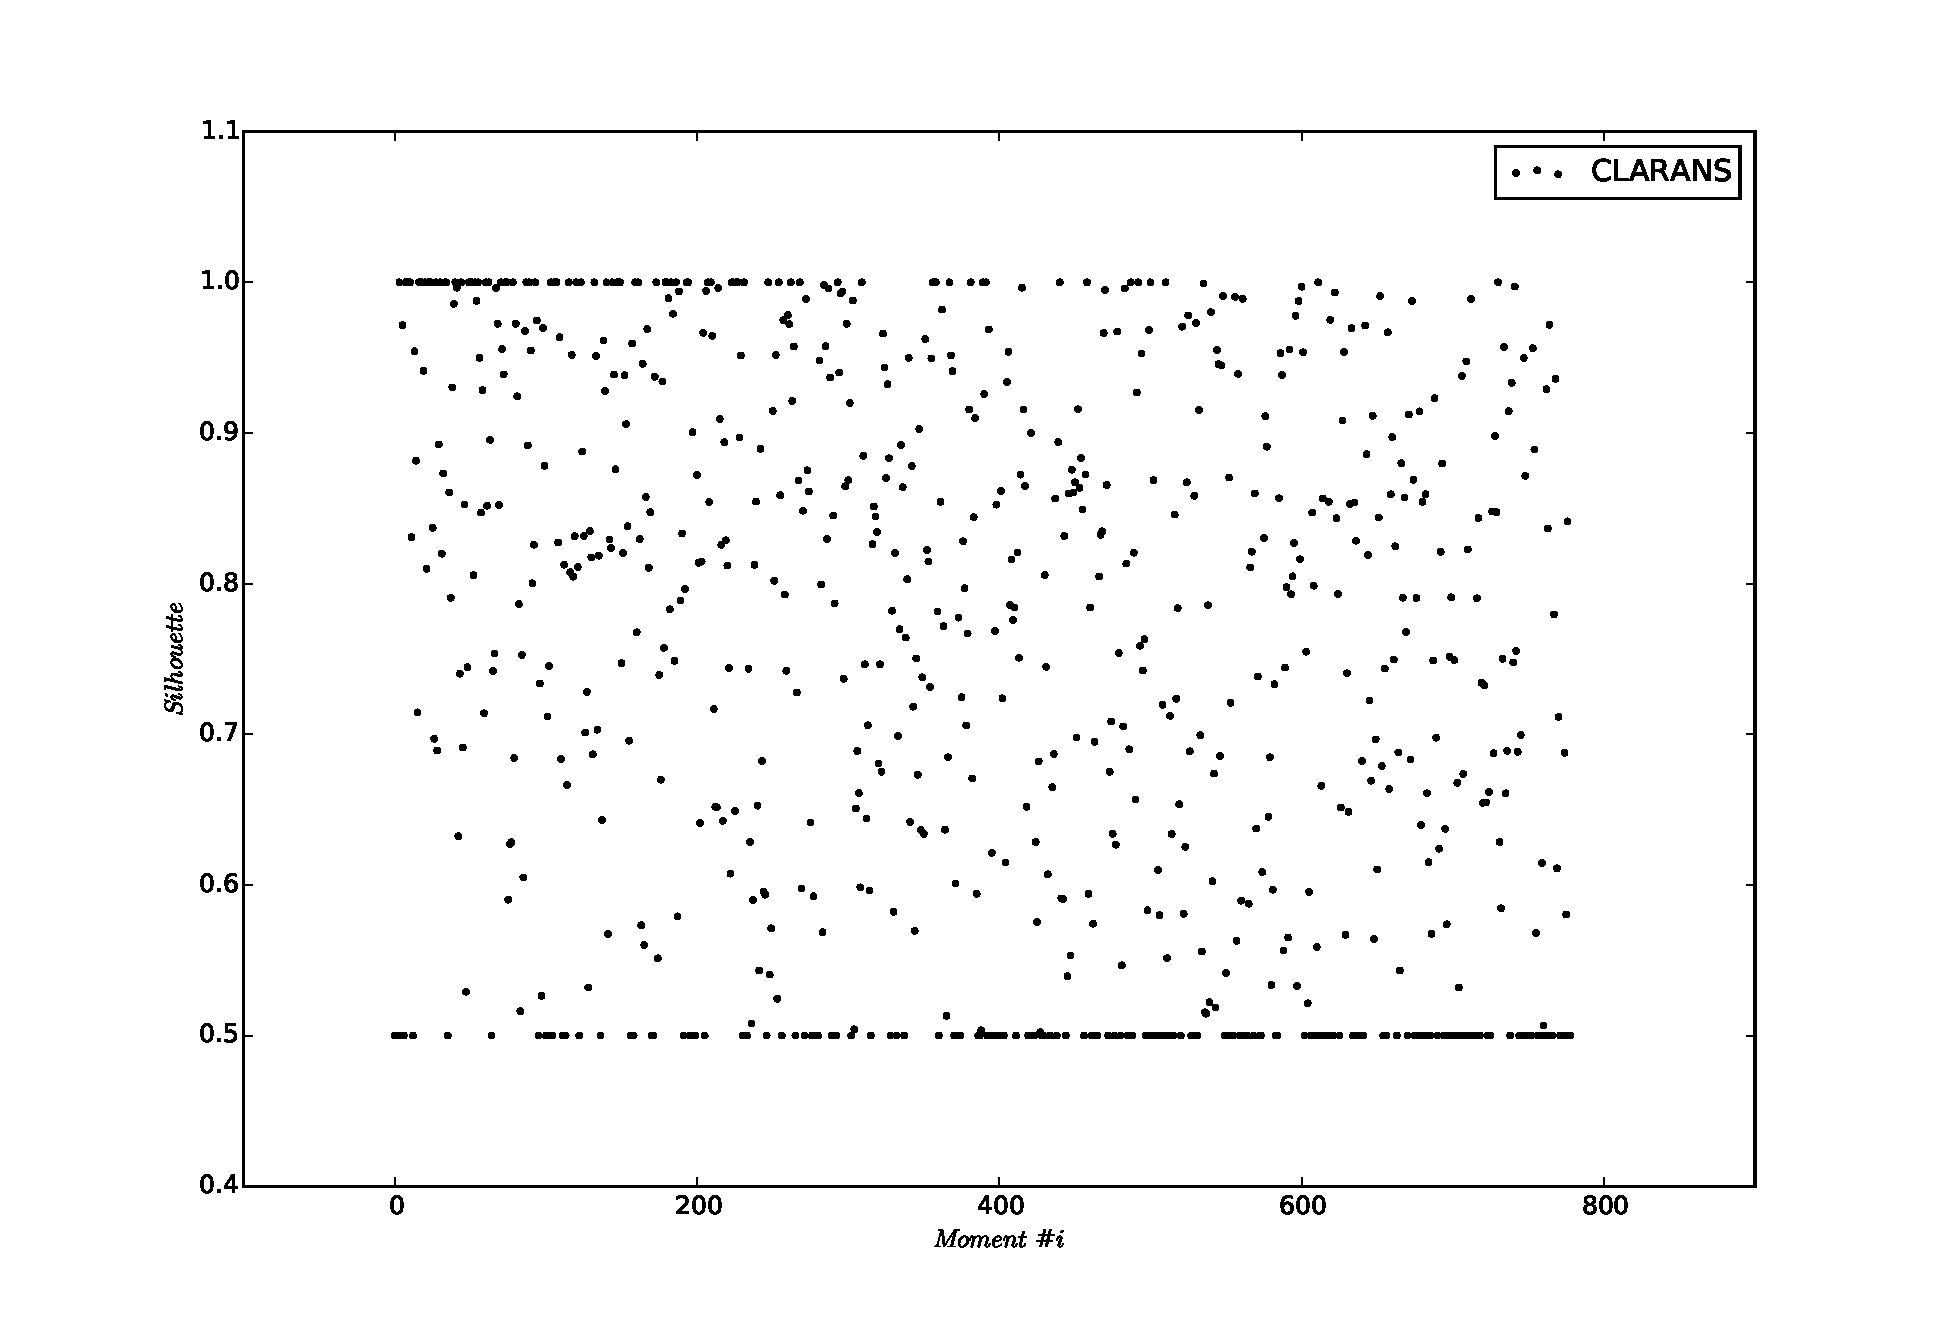
\includegraphics[width=0.9\textwidth]{plots/clarans_silhouette.pdf}
    \caption{Moment-wise silhouette coefficients for CLARANS.
    \label{fig:clarans-silhouette} }
\end{figure}

\begin{figure}[ht]
    \centering
    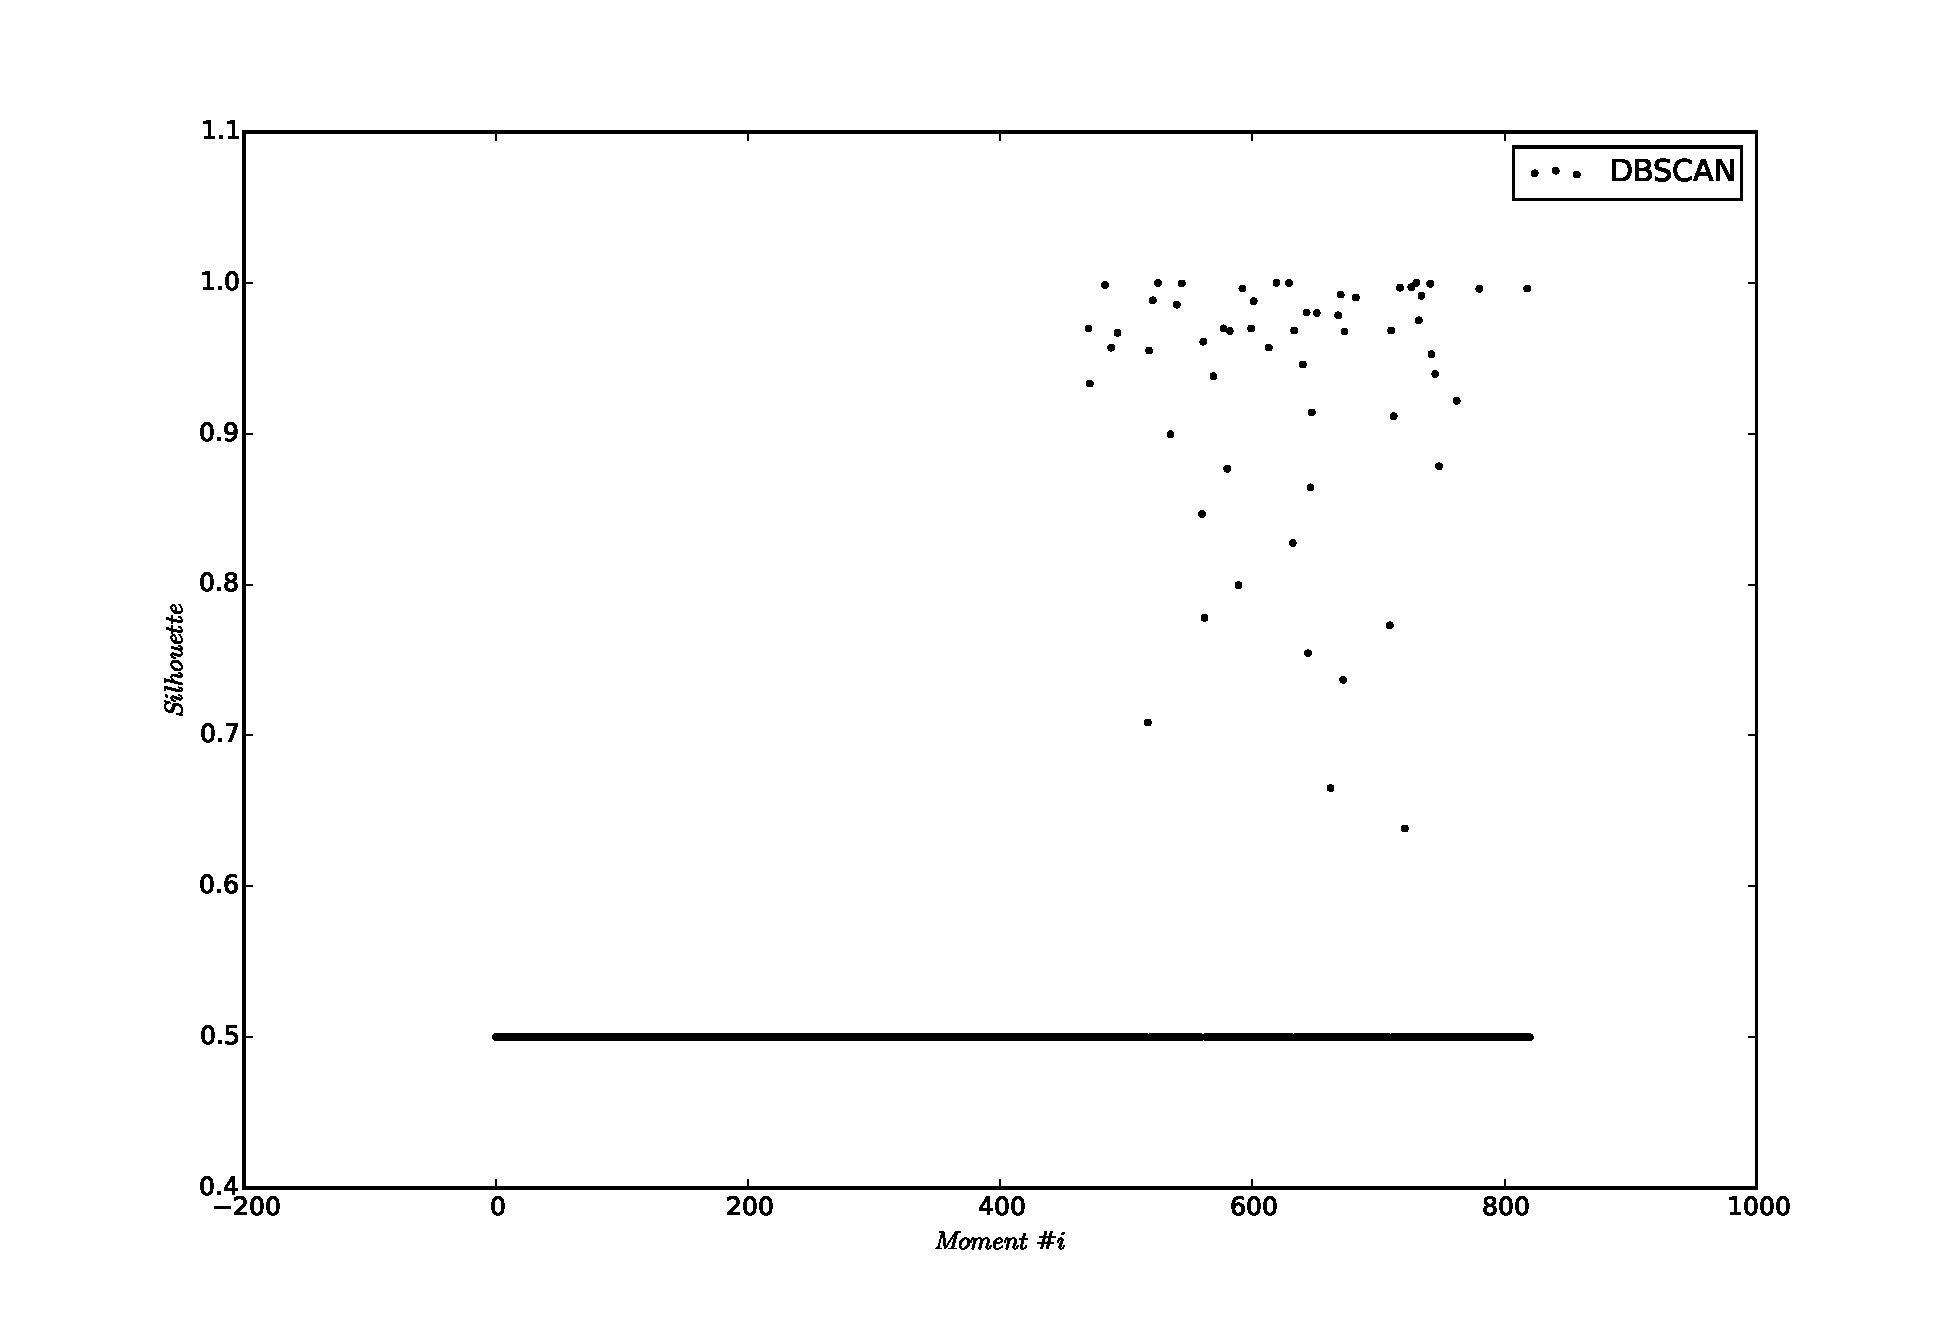
\includegraphics[width=0.9\textwidth]{plots/dbscan_silhouette.pdf}
    \caption{Moment-wise silhouette coefficients for DBSCAN.
    \label{fig:dbscan-silhouette} }
\end{figure}

\begin{figure}[ht]
    \centering
    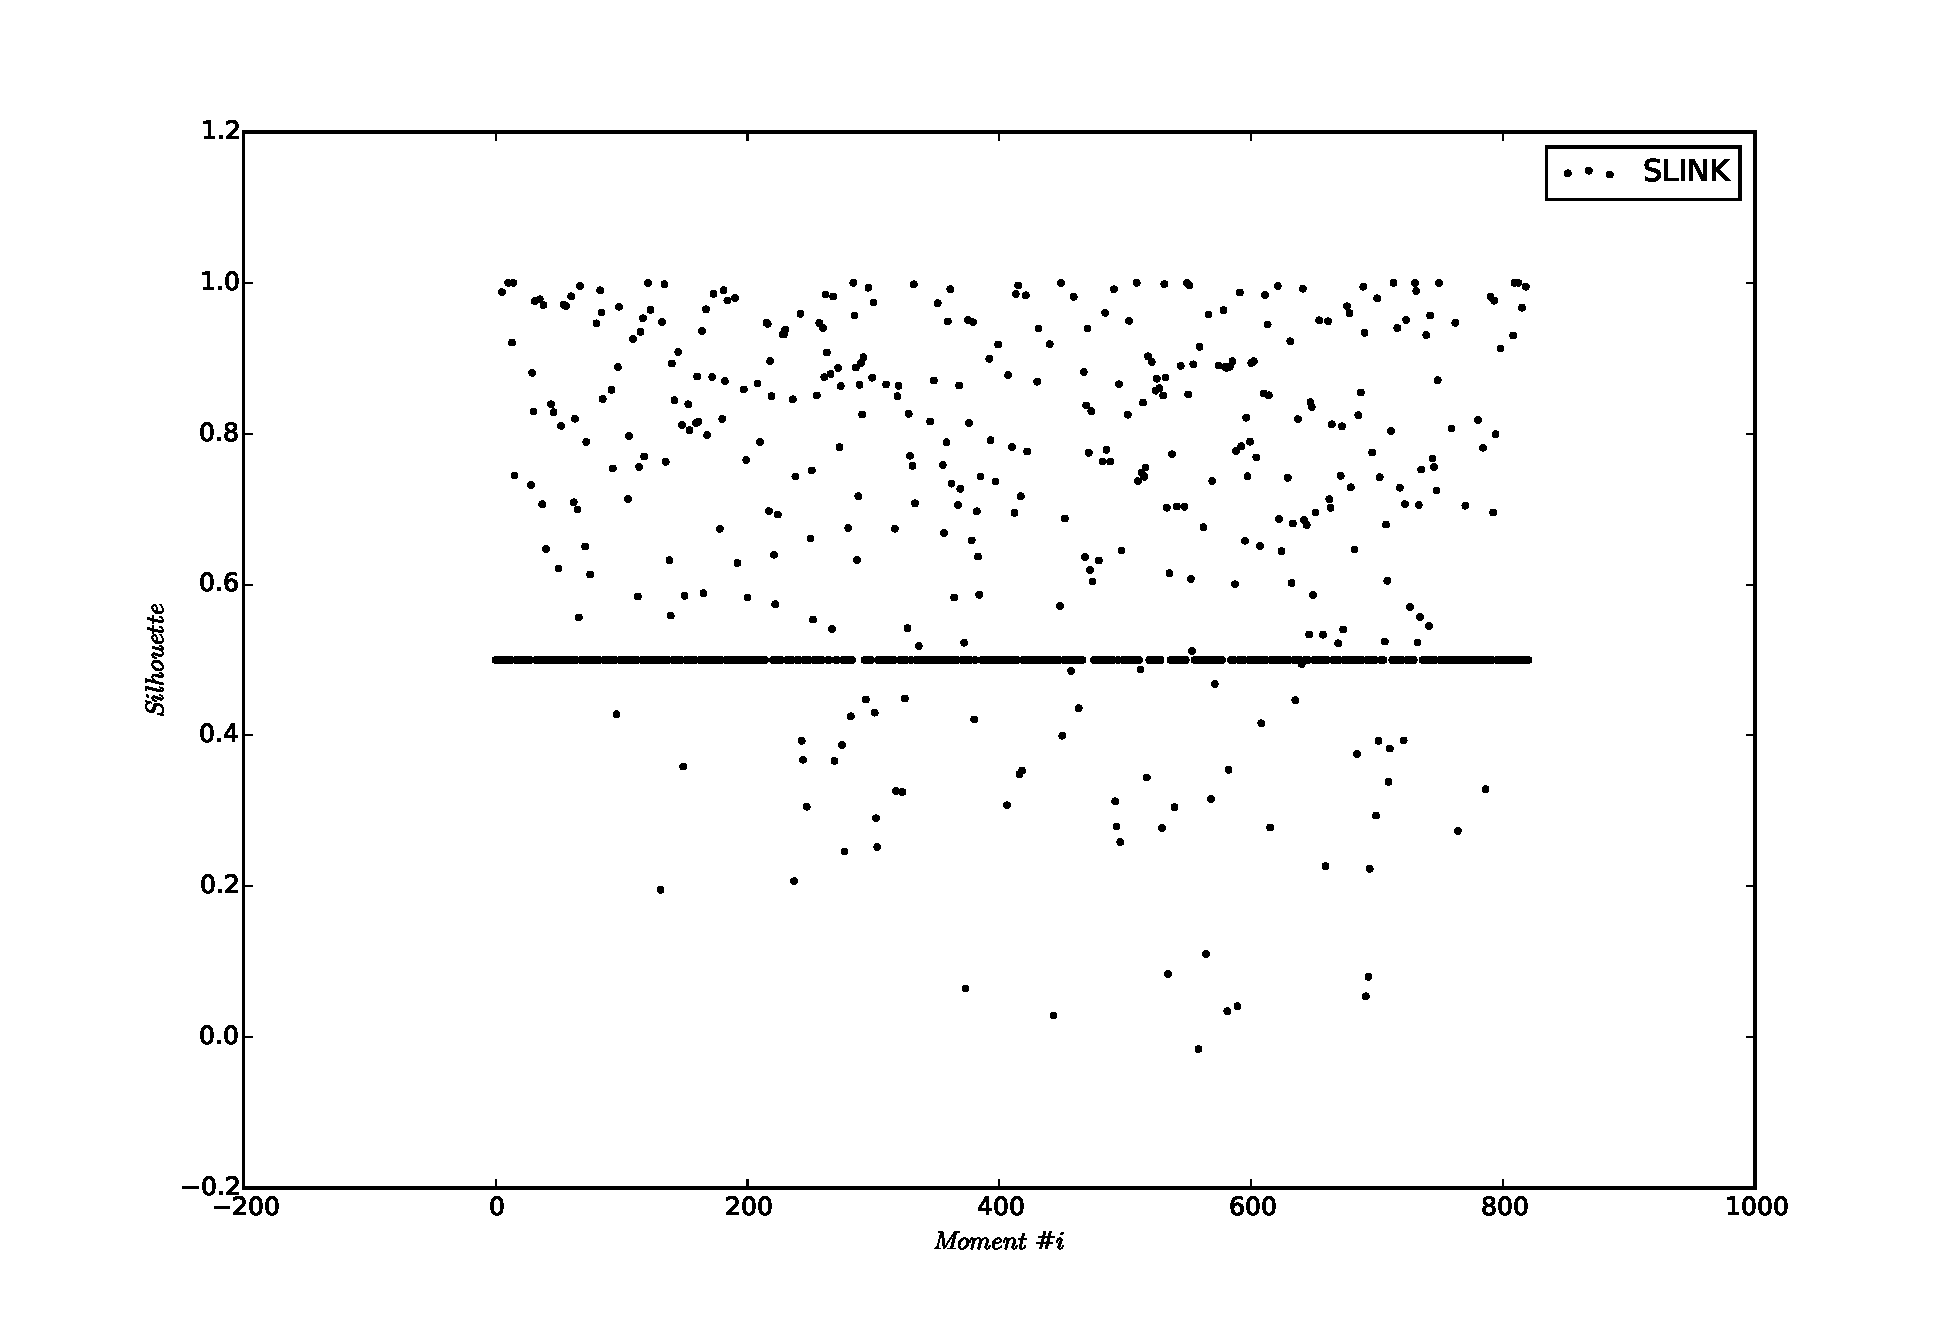
\includegraphics[width=0.9\textwidth]{plots/slink_silhouette.pdf}
    \caption{Moment-wise silhouette coefficients for SLINK.
    \label{fig:slink-silhouette} }
\end{figure}

\begin{table}
    \centering
    {\begin{tabular}{ | l | l | c c c c | }
        \hline
        Algorithm & Mean SC        & Strong & Reasonable & Weak & No  \\
        \hline
        CLARANS   & 0.751818981799 & 457    & 167        & 155  & 0  \\
        DBSCAN    & 0.529126434287 & 54     & 2          & 765  & 0  \\
        SLINK     & 0.608986935167 & 250    & 69         & 486  & 16 \\
        \hline
    \end{tabular}}
    \caption{Mean silhouette coefficient per algorithm in the data set, and
        quantities within each defined Silhouette interpretation area.} 
    \label{table:mean-silhouette}
\end{table}

The Silhouette coefficients are plotted with the Moments sorted from 
the smallest number of data points to the largest, shown in 
figure~\ref{fig:clarans-silhouette}, figure~\ref{fig:dbscan-silhouette}
and figure~\ref{fig:slink-silhouette}. The sorting is intended
to visualize any potential correlation between the number of data points 
in a set, and the clustering results with regard to Silhouette coefficients.

The mean value of each plot is provided as a more comprehensible reference 
value in table~\ref{table:mean-silhouette}, along with the quantities of
coefficients with in each interpretation category, 
as suggested by \citeauthor{silhouettes}.

\cleartoleftpage

\subsection{Larger Data Set Activity Detection}
This section addresses data set consisting of $59$ photo sequences
grouped by user id's, ranging 
from $200$ data points to thousands in each set. All three algorithms
have been given an attempt to cluster each photo sequence. The \emph{haversine} 
method is used for distance measurements. A computation is aborted if 
it takes longer than $60$ seconds. Results are 
excluded from a algorithms computation result set if it did not finish
in time. In total, CLARANS timed out on $19$ of the Moments, and 
DBSCAN and SLINK did the same with $1$ each. In this data sets, multiple
clusters are likely to be present, as it contains several Moments in 
each data set. 

\subsubsection{Performance}

\begin{figure}[ht]
    \centering
    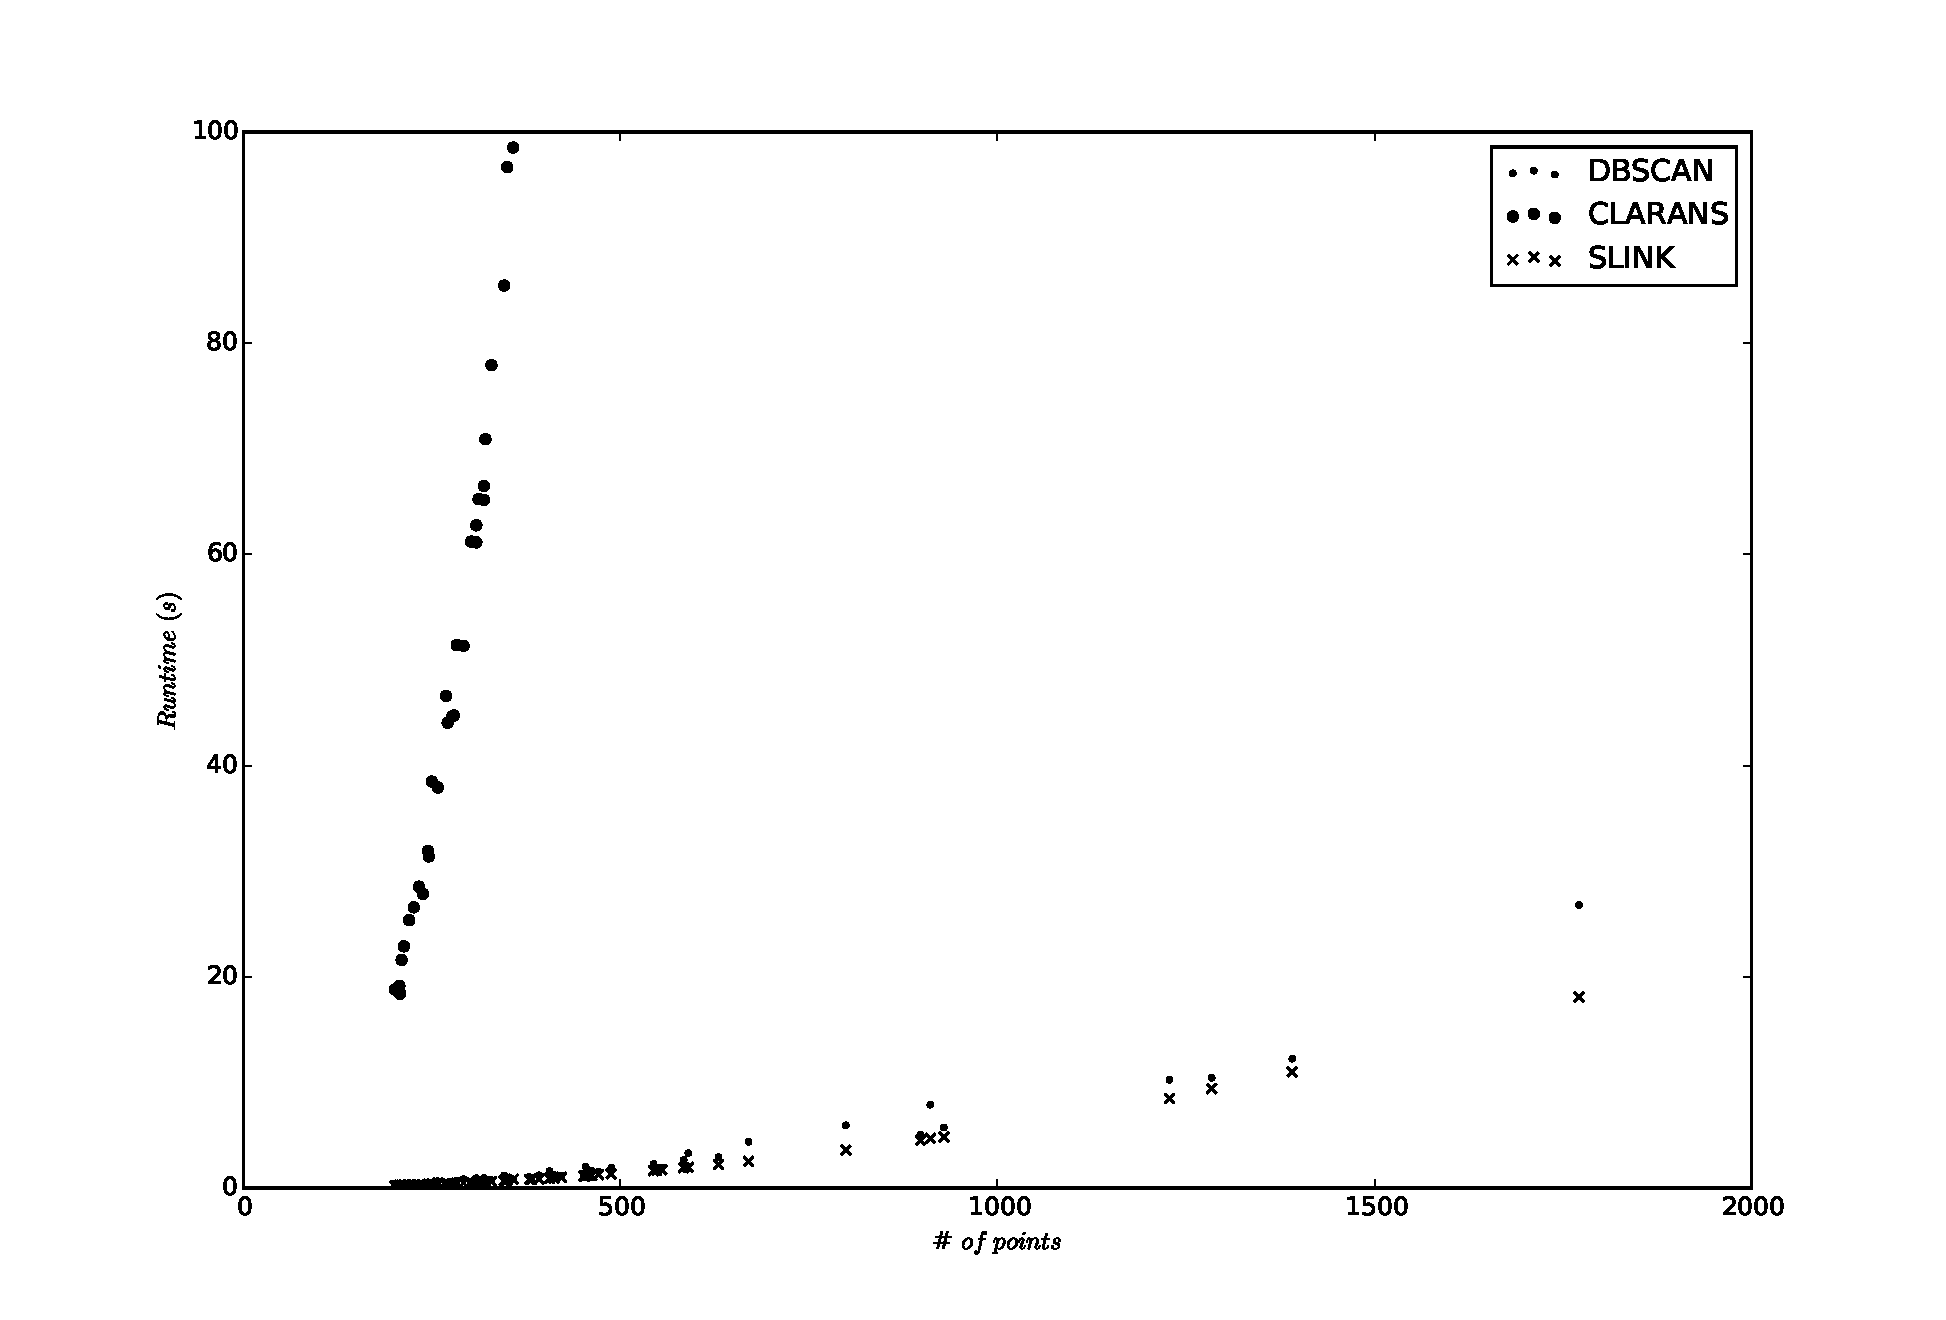
\includegraphics[width=0.7\textwidth]{plots/days_runtime_scatter.pdf}
    \caption{Run-time for clustering algorithms over users days, by number of
        points on the day.
    \label{fig:day-runtime-scatter} }
\end{figure}

The plot depicting run-time in figure~\ref{fig:day-runtime-scatter} now 
shows somewhat smaller spectrum of the x-axis.

\clearpage

\subsubsection{Silhouettes}

The Silhouettes have not changed from the smaller data set in any particular
manner, and are therefore shown here for completeness.

\begin{table}
    \centering
    {\begin{tabular}{ | l | l | c c c c | }
        \hline
        Algorithm & Mean SC & Strong & Reasonable & Weak & No  \\
        \hline
        CLARANS & 0.783864065615 & 19 & 9 & 2  & 0  \\
        DBSCAN  & 0.581829108024 & 10 & 0 & 48 & 0  \\
        SLINK   & 0.63724366955  & 20 & 6 & 32 & 0  \\
        \hline
    \end{tabular}}
    \caption{Mean silhouette coefficient per algorithm in the larger data set, and
        quantities within each defined Silhouette interpretation area.} 
    \label{table:days-mean-silhouette}
\end{table}

\begin{figure}[h!]
    \centering
    \begin{subfigure}[b]{0.45\textwidth}
        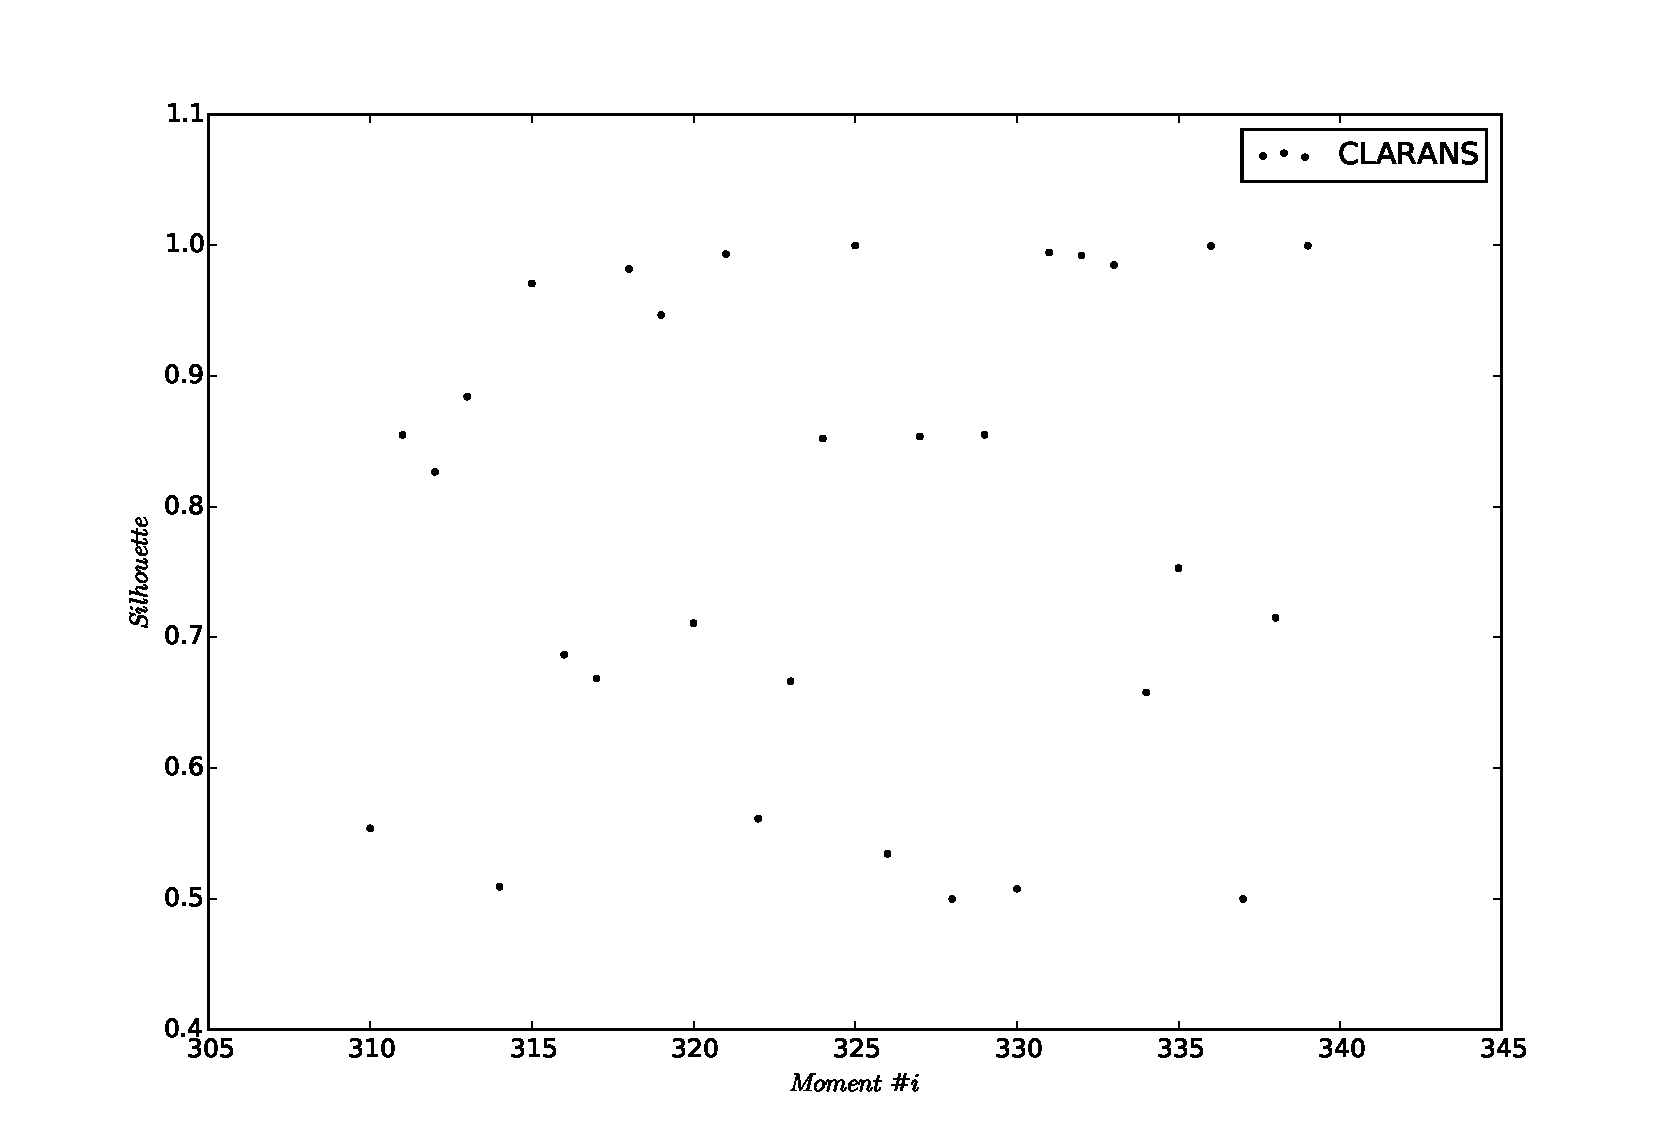
\includegraphics[width=\textwidth]{plots/days_clarans_silhouette.pdf}
        \caption{Moment-wise silhouette coefficients for CLARANS for a larger 
        data set. }
        \label{fig:days-clarans-silhouette}
    \end{subfigure}%
    ~
    \begin{subfigure}[b]{0.45\textwidth}
        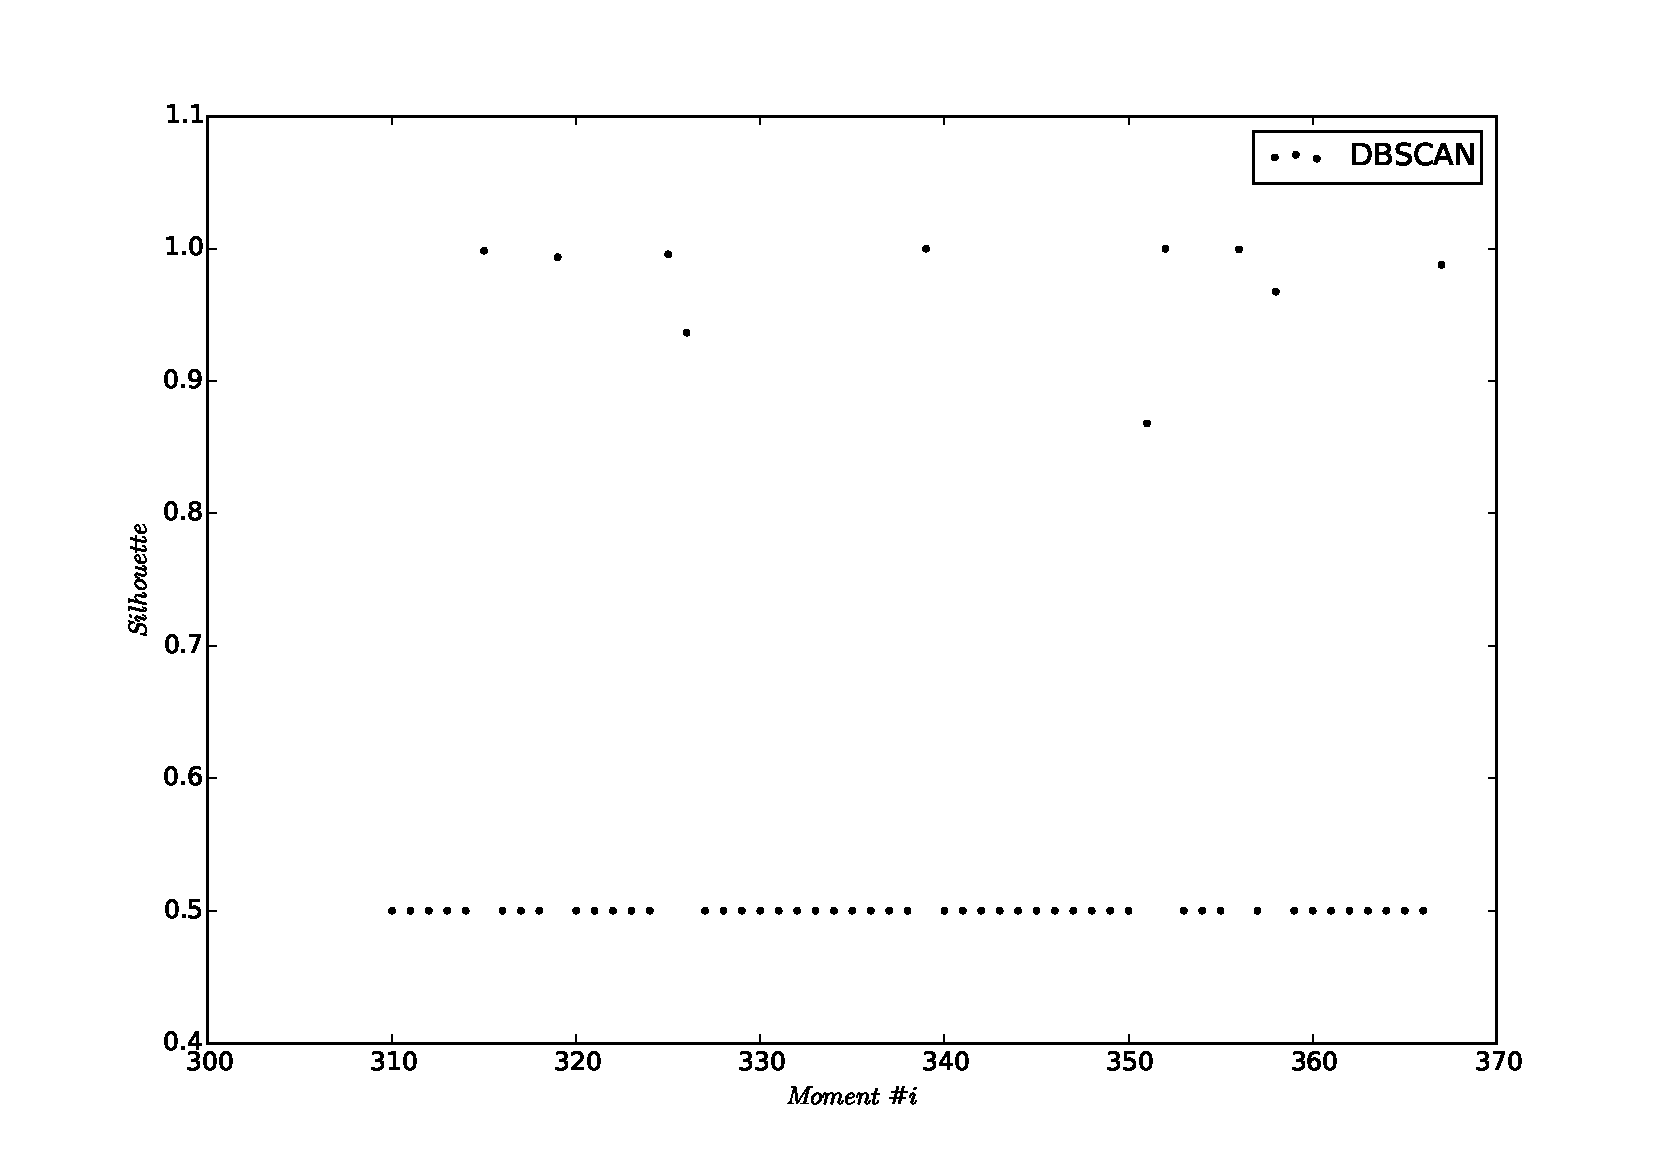
\includegraphics[width=\textwidth]{plots/days_dbscan_silhouette.pdf}
        \caption{Moment-wise silhouette coefficients for DBSCAN for a larger 
        data set. }
        \label{fig:days-dbscan-silhouette}
    \end{subfigure}
    
    \begin{subfigure}[b]{0.45\textwidth}
        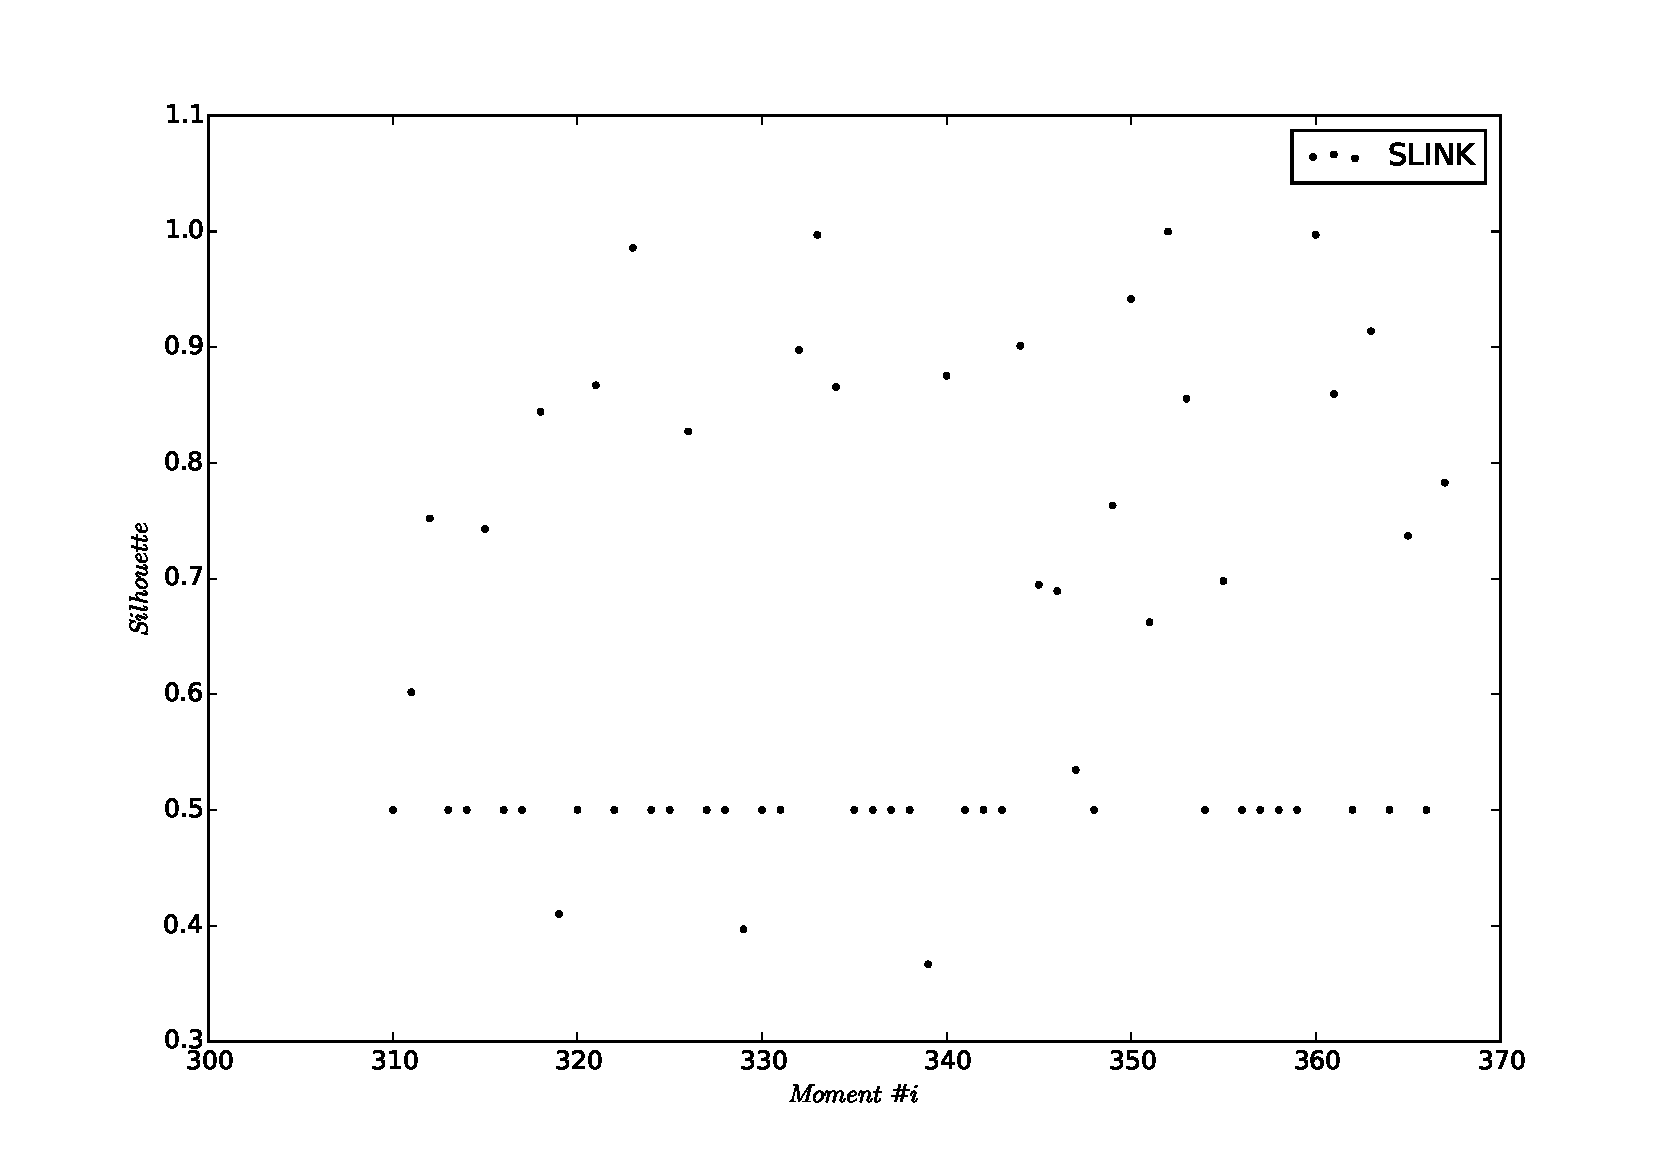
\includegraphics[width=\textwidth]{plots/days_slink_silhouette.pdf}
        \caption{Moment-wise silhouette coefficients for SLINK for a larger 
        data set. }
        \label{fig:days-slink-silhouette}
    \end{subfigure}
\end{figure}

\cleartoleftpage

\subsection{Cluster Detection Comparison}
Different clustering methods result in different clusterings. As an 
attempt to illustrate this, comparisons displaying different clustering
methods and the number of clusters detected in each data set is plotted 
in this section. The regarded data sets are sorted in increasing order 
based on the number of data points in each set.

Although figure~\ref{fig:dbscan-vs-clarans}, \ref{fig:dbscan-vs-slink}
and\ref{fig:clarans-vs-slink} seem somewhat cluttered, the intention here is 
to show the difference in numbers of detected clusters as the data set
increases.

\begin{figure}[ht]
    \centering
    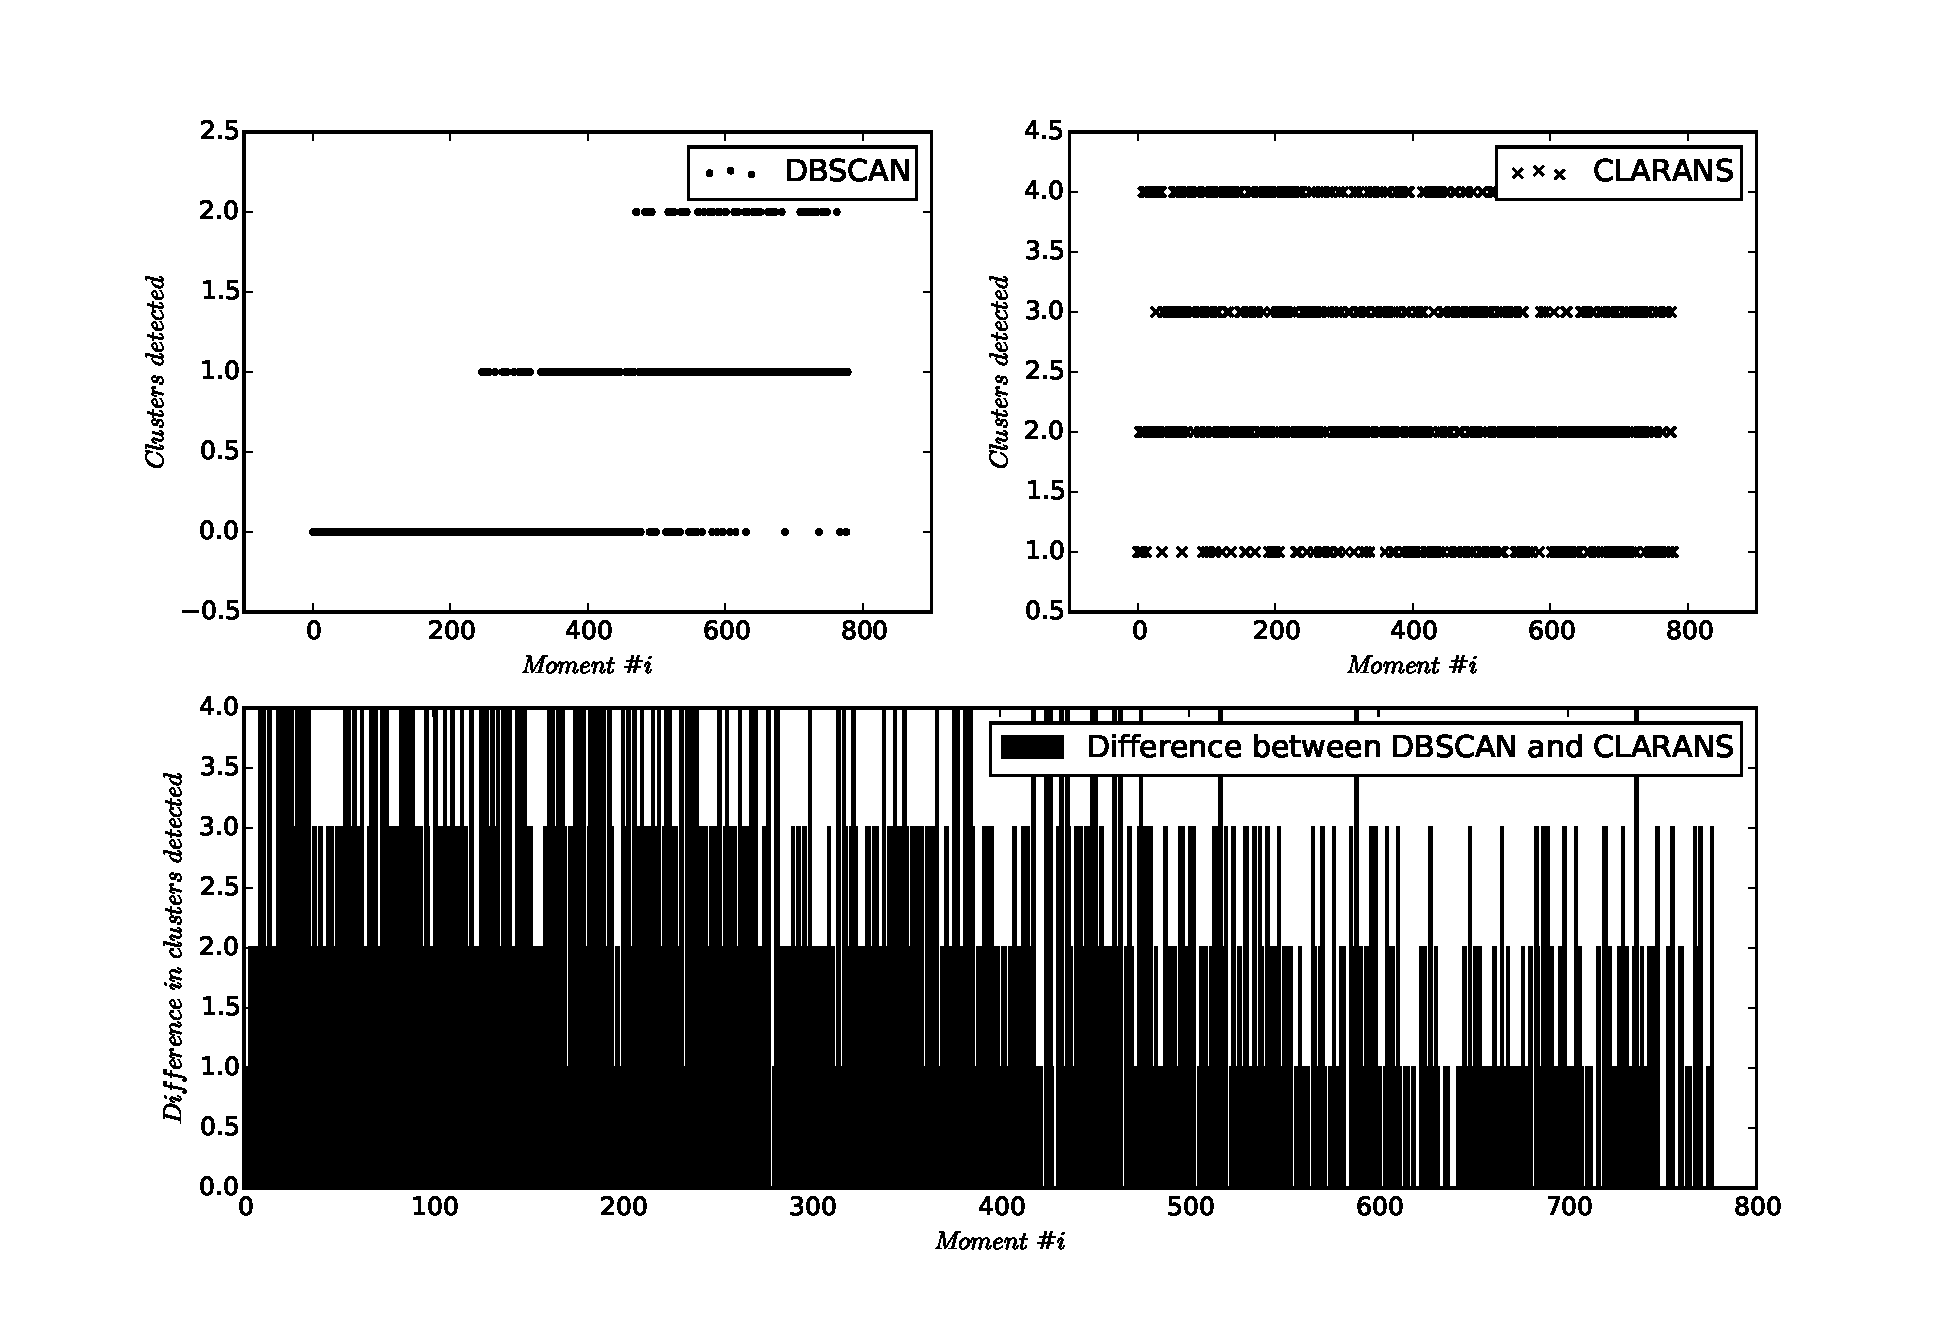
\includegraphics[width=0.9\textwidth]{plots/dbscan_vs_clarans.pdf}
    \caption{Cluster detection, comparison between DBSCAN and CLARANS.
    \label{fig:dbscan-vs-clarans} }
\end{figure}

\begin{figure}[ht]
    \centering
    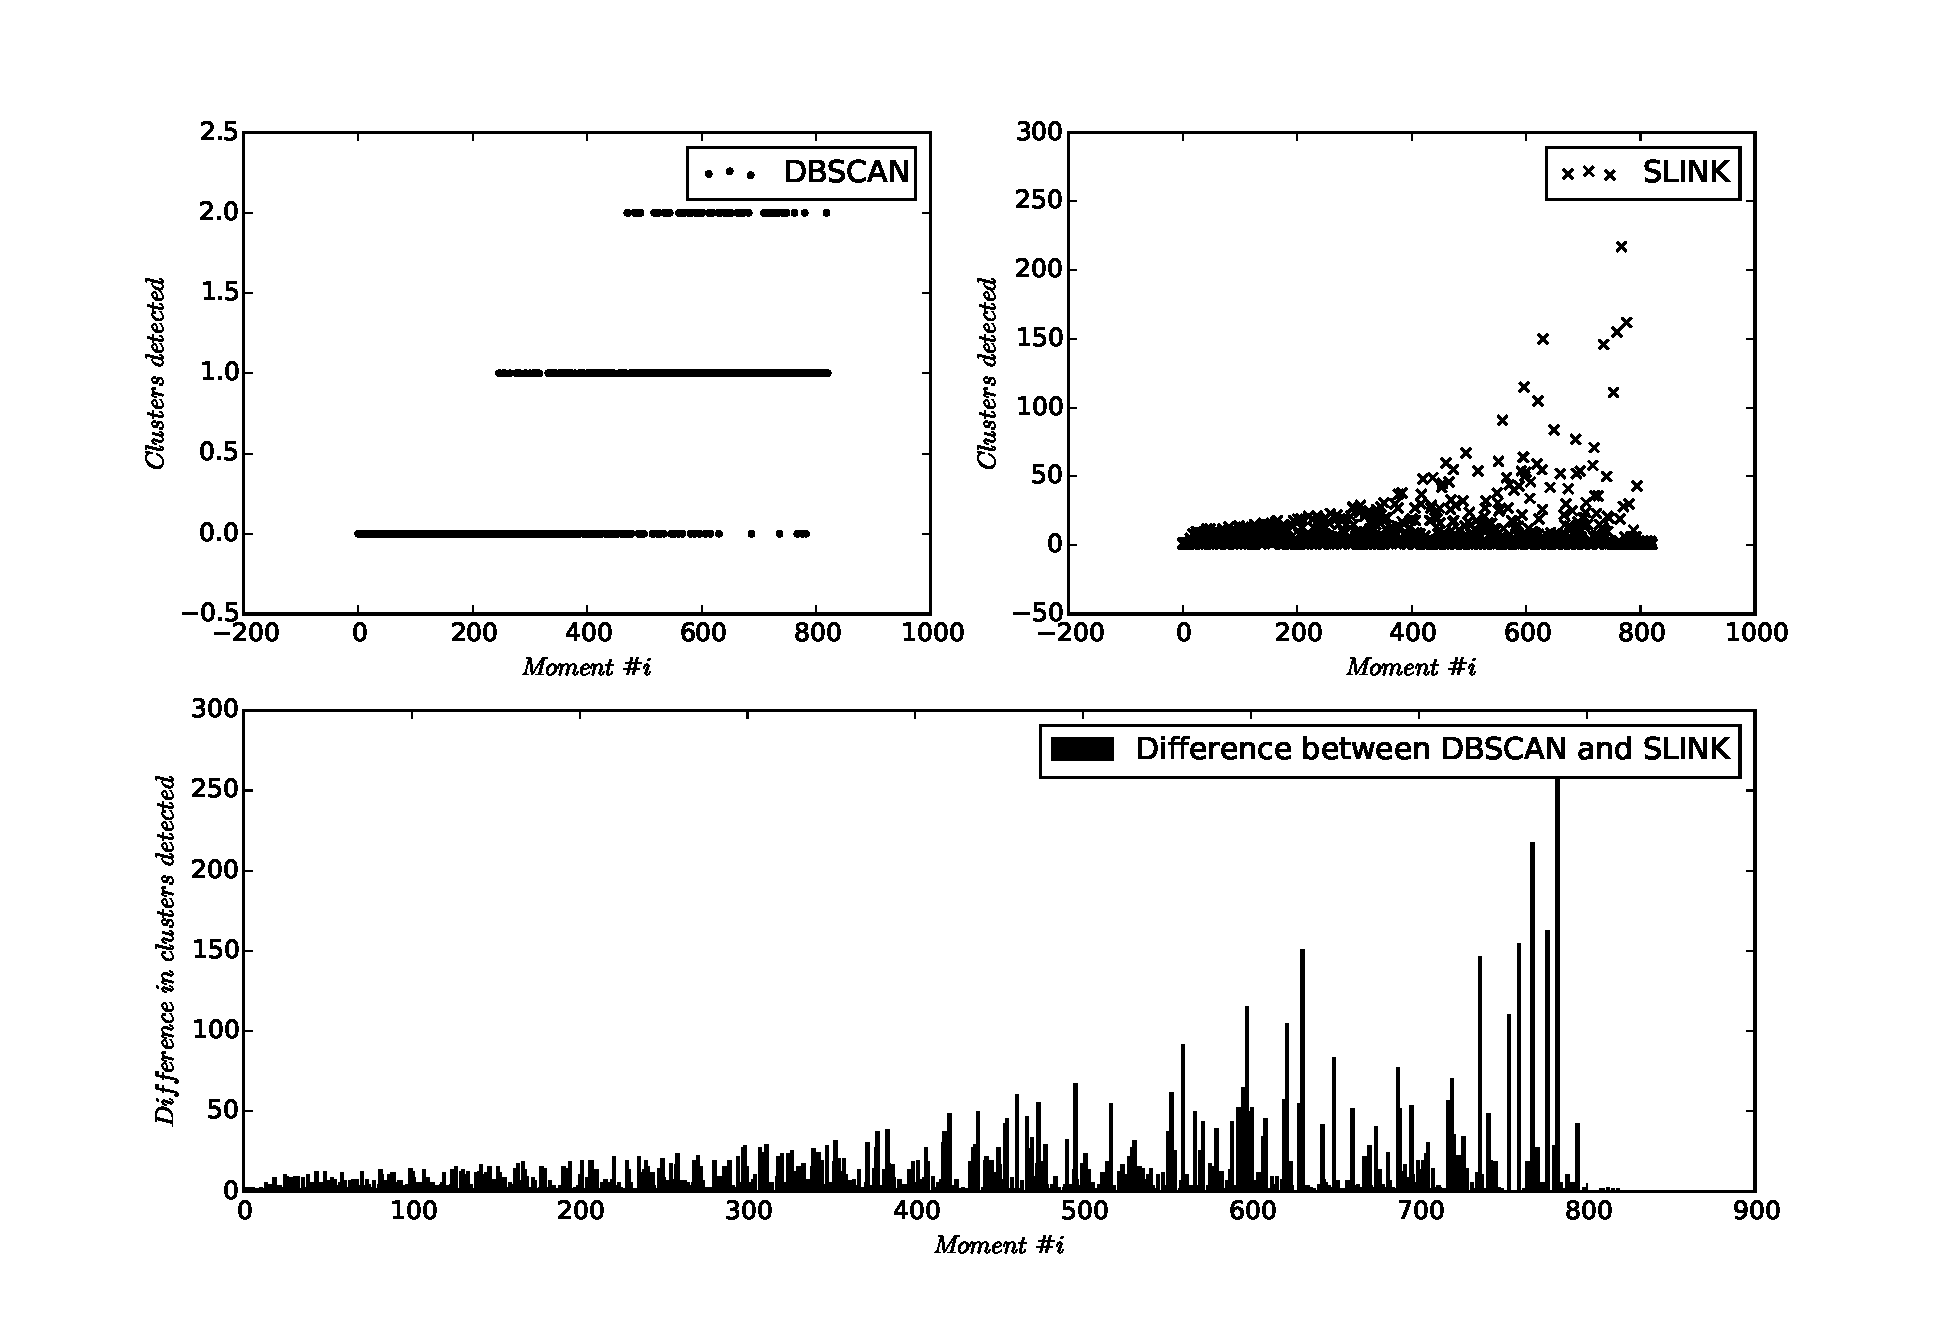
\includegraphics[width=0.9\textwidth]{plots/dbscan_vs_slink.pdf}
    \caption{Cluster detection, comparison between DBSCAN and SLINK.
    \label{fig:dbscan-vs-slink} }
\end{figure}

\begin{figure}[ht]
    \centering
    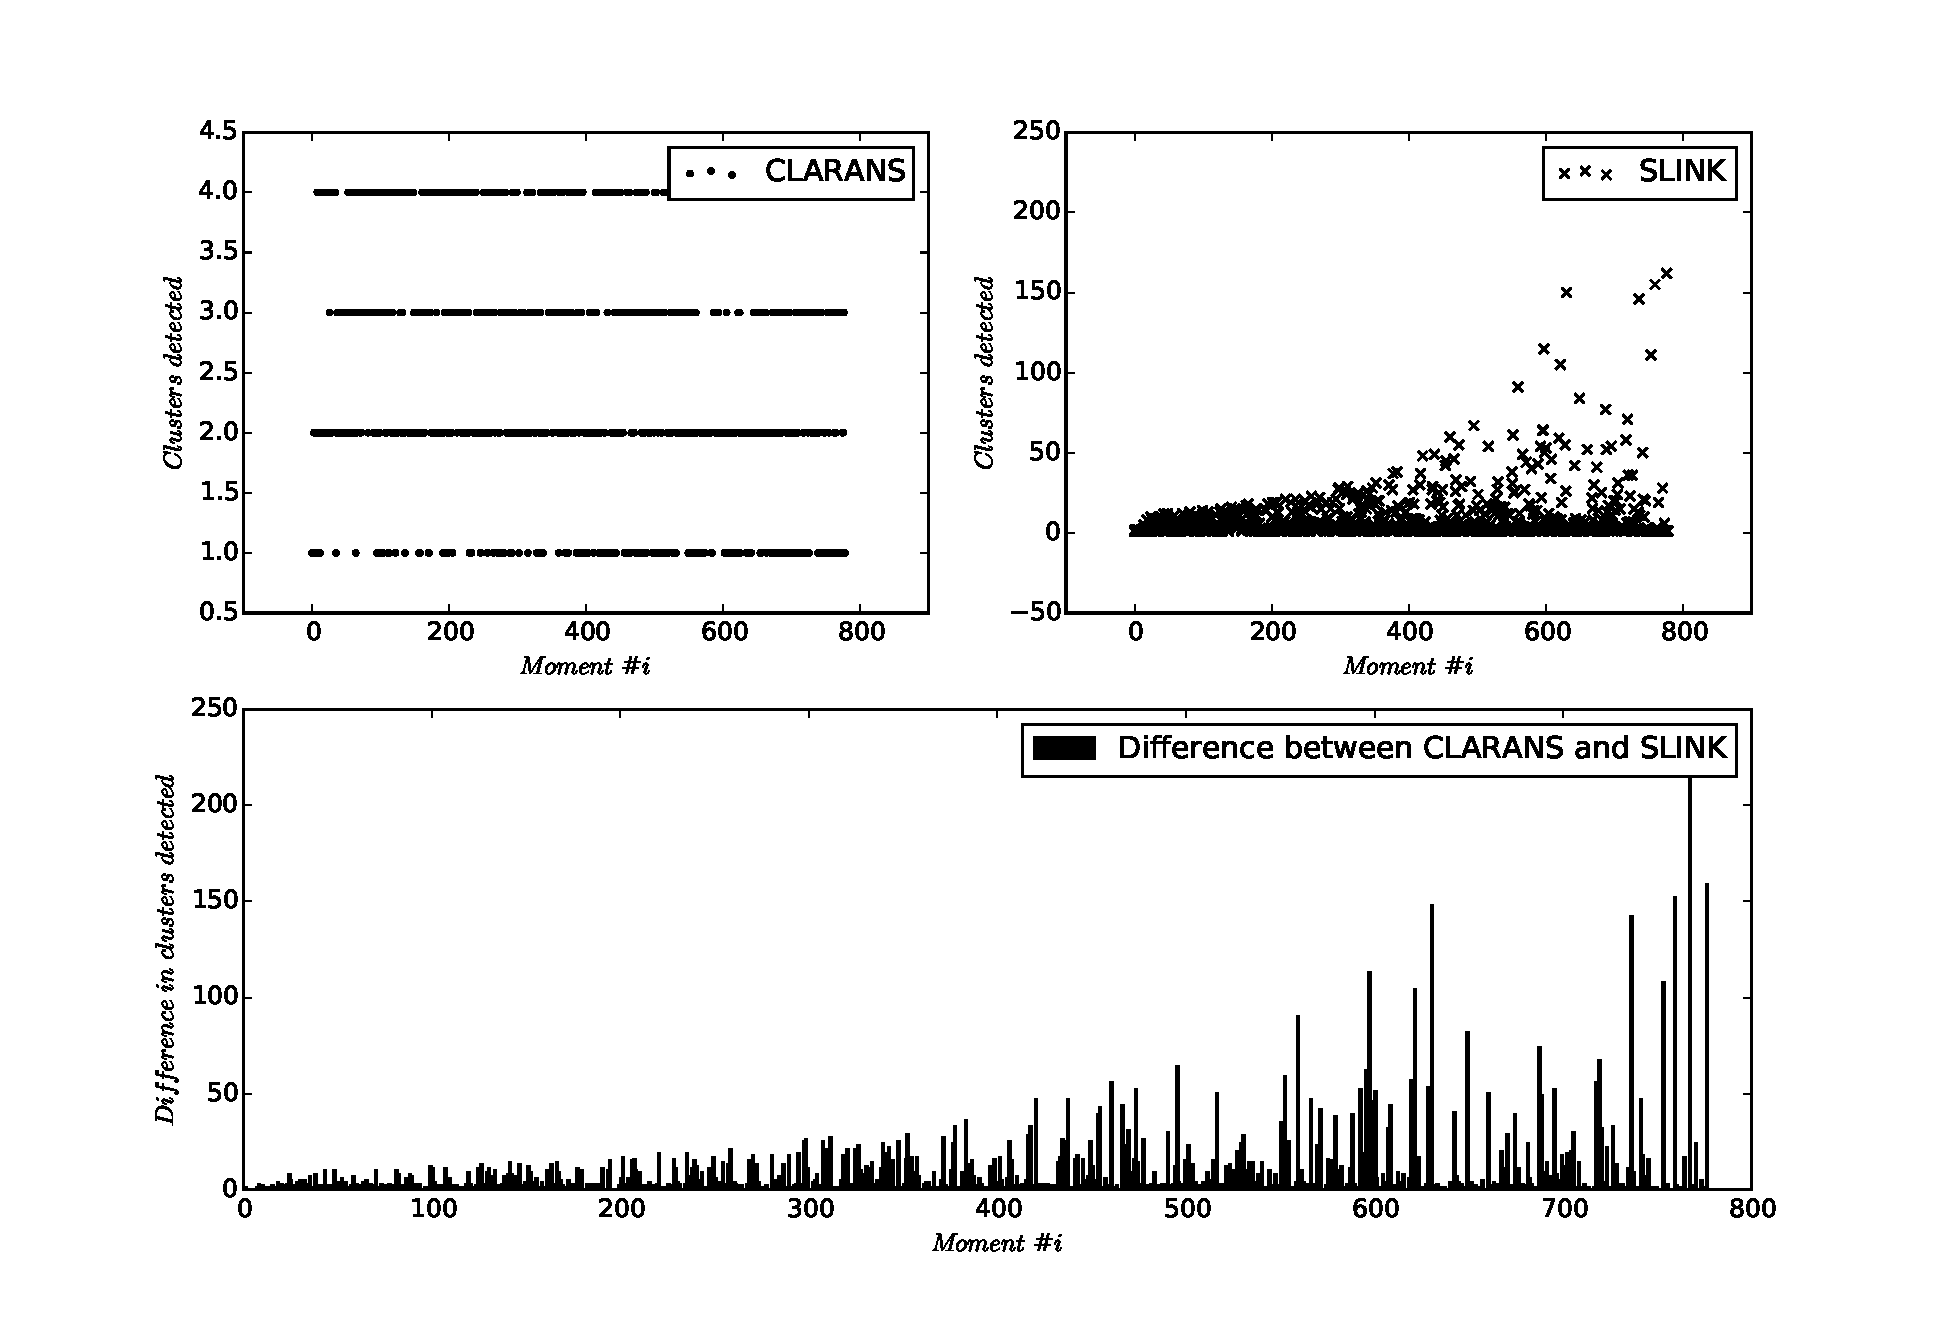
\includegraphics[width=0.9\textwidth]{plots/clarans_vs_slink.pdf}
    \caption{Cluster detection, comparison between CLARANS and SLINK.
    \label{fig:clarans-vs-slink} }
\end{figure}

\cleartoleftpage

\section{Classification}
The classification is conducted after an initial activity detection, in 
this case the above shown spatial clustering. In this stage, the activity
detection is considered correct and which type of clustering algorithm 
that is used is ignored, as all considered and approved algorithms should 
be able to produce desired clusters.

\subsection{Data Set}
The survey based on the user polling in the proof-of-concept implementation
was conducted internally at Narrative.

A total of 11 people participated, and contributed to a total of 62 evaluated
Moment classifications. 

Taking all this into account, it is assumed that the data set still contains 
sufficient and a diverse enough user base to draw conclusions. 

\subsection{Evaluation Overview}

\begin{table}
    \centering
    {\begin{tabular}{ | l | c | l | c | l | c | l | c |}
        \hline
            \multicolumn{2}{|c|}{Movement} &
            \multicolumn{2}{|c|}{Social}   &
            \multicolumn{2}{|c|}{Working}  &
            \multicolumn{2}{|c|}{Indoors} \\
        \hline
            \multicolumn{8}{|c|}{User-assigned values} \\
        \hline
        Stationary  & 40 & Social & 53 & Working    & 57 & Indoors  & 38 \\
        Moving      & 23 & Alone  & 16 & Off Hours  & 12 & Outdoors & 31 \\
        Exercising  &  6 &        &    &            &    &          &    \\
        \hline
            \multicolumn{8}{|c|}{Algorithm-assigned values} \\
        \hline
        Stationary  & 51 & Social & 22 & Working    & 39 & Indoors  & 69 \\
        Moving      & 18 & Alone  & 48 & Off Hours  & 31 & Outdoors & 1 \\
        Exercising  &  1 &        &    &            &    &          &    \\
        \hline
            \multicolumn{8}{|c|}{Correctly assigned according to users.} \\
        \hline
            \multicolumn{2}{|c|}{75.81\%} &
            \multicolumn{2}{|c|}{54.84\%} &
            \multicolumn{2}{|c|}{56.45\%} &
            \multicolumn{2}{|c|}{54.84\%} \\
        \hline
    \end{tabular}}
    \caption{Classification results.} 
    \label{table:classification-values}
\end{table}

\begin{table}
    \centering
    {\begin{tabular}{ | l | c | c |}
        \hline
            Category & False Positive & False Negative \\
        \hline
        Movement    & 1  & 12 \\
        Social      & 0  & 31 \\
        Working     & 27 & 1  \\
        Indoors     & 0  & 31 \\
        \hline
    \end{tabular}}
    \caption{False positives and negatives.} 
    \label{table:false-values-before}
\end{table}

The results after the users responded to the poll is presented in 
table~\ref{table:classification-values}. The quantities 
of assigned classifications by users are shown in the top part of the
table, out of the $69$ assessed Moments. So, for instance, in the 
Movement category there were $40$ Moments assigned as Stationary, 
$23$ as Moving and $6$ as Exercising. In the same manner below that, 
the algorithms assignments to different classes is presented. Note that
this is not the same amount, as these are based on activities, and there
can be (but rarely are) several activities in a Moment.

Table~\ref{table:false-values-before} presents the false negatives and 
positives within each category. The correct assignments are not included
in this table, as only wrong assignments can provide false negatives
and false positives.

\subsection{Second Run}

\begin{table}
    \centering
    {\begin{tabular}{ | l | c | l | c | l | c | l | c |}
        \hline
            \multicolumn{2}{|c|}{Movement} &
            \multicolumn{2}{|c|}{Social}   &
            \multicolumn{2}{|c|}{Working}  &
            \multicolumn{2}{|c|}{Indoors} \\
        \hline
            \multicolumn{8}{|c|}{User-assigned values} \\
        \hline
        Stationary  & 40 & Social & 53 & Working    & 57 & Indoors  & 38 \\
        Moving      & 23 & Alone  & 16 & Off Hours  & 12 & Outdoors & 31 \\
        Exercising  &  6 &        &    &            &    &          &    \\
        \hline
            \multicolumn{8}{|c|}{Algorithm-assigned values} \\
        \hline
        Stationary  & 45 & Social & 27 & Working    & 26 & Indoors  & 44 \\
        Moving      & 18 & Alone  & 43 & Off Hours  & 44 & Outdoors & 26 \\
        Exercising  &  7 &        &    &            &    &          &    \\
        \hline
            \multicolumn{8}{|c|}{Correctly assigned according to users.} \\
        \hline
            \multicolumn{2}{|c|}{78.57\%} &
            \multicolumn{2}{|c|}{62.85\%} &
            \multicolumn{2}{|c|}{73.21\%} &
            \multicolumn{2}{|c|}{71.43\%} \\
        \hline
    \end{tabular}}
    \caption{Classification results after model modification and learning. } 
    \label{table:classification-after-values}
\end{table}

The table~\ref{table:classification-after-values} presents its results in the
same manner as table~\ref{table:classification-values}, but after modification 
of the model via Bayesian learning and lessons learnt after the first user tests. 
The upper area containing the  users assignments remain the same as in 
table~\ref{table:classification-values}, but is kept in this table as well 
for easier reference.

\begin{table}
    \centering
    {\begin{tabular}{ | l | c | c |}
        \hline
            Category & False Positive & False Negative \\
        \hline
        Movement    & 1     & 12 \\
        Social      & 0     & 26 \\
        Working     & 14    & 4  \\
        Indoors     & 7     & 13 \\
        \hline
    \end{tabular}}
    \caption{False positives and negatives after model modification and learning. } 
    \label{table:false-values-after}
\end{table}

In the same way, table~\ref{table:false-values-after} depicts false negatives and 
positives during the run within each category, after the model had been altered.

\clearpage

\subsection{User Grades}

\begin{table}
    \centering
    {\begin{tabular}{ | c | c | c | c | c | c | c | }
        \hline
        Grade & Assigned & Mean &
        \multicolumn{2}{|c|}{False Positive} &
        \multicolumn{2}{|c|}{False Negative} \\
        \hline
        5 & 22 & 0.00 & 0  & 0.00  & 0  & 0.00 \\
        4 & 16 & 1.19 & 4  & 0.25  & 15 & 0.94 \\
        3 & 13 & 2.15 & 8  & 0.62  & 20 & 1.54 \\
        2 & 16 & 2.88 & 14 & 0.88  & 32 & 2.00 \\
        1 & 2  & 3.00 & 2  & 1.00  & 4  & 2.00 \\
        \hline
    \end{tabular}}
    \caption{False positives and negatives correlated
        with user-assigned grades. } 
    \label{table:false-values-vs-grades}
\end{table}

\begin{table}
    \centering
    {\begin{tabular}{ | l | c | c | c | c | c | c | }
        \hline
        User & Count & Mean Grade\\
        \hline
        User \#1 & 17 & 4.47 \\
        User \#2 & 7  & 3.14 \\
        User \#3 & 12 & 3.33 \\
        User \#4 & 8  & 3.5  \\
        User \#5 & 7  & 4.0  \\
        User \#6 & 8  & 2.63 \\
        \hline
    \end{tabular}}
    \caption{Mean grades and number of classifications distributed 
        among the users with most responses.} 
    \label{table:user-wise-mean-grade}
\end{table}

\emph{
    The reason that the number of values in the Assigned column
    of table~\ref{table:false-values-vs-grades} does not sum to
    62 as the number of examined Moments were, is simply that these
    are scores for each activity, not for each Moment assessed, as 
    there can be several activities in a Moment. }

Table~\ref{table:false-values-vs-grades} shows the correlation 
between false positives and negatives, along with the grades 
that users have assigned to the classification. 
The column marked mean shows the mean number of errors in order a
classification getting the corresponding user grade. The first value 
in the false-columns shows the total number of false positives 
and negatives respectively in classifications that have received 
a certain grade. The real-valued column shows the number of false 
positives respectively per classification in that category. 


\chapter{Discussion}
\label{ch:discussion}

\section{Clustering Comparison}
The three representatives were, as initially mentioned, chosen from each 
classical branch of clustering algorithm. The results more or less confirm
what is expected from the theoretical background, and enhances the 
conviction of the suitability of different algorithms.

\subsection{Performance}
When comparing the run-time of the three assessed algorithms by 
consulting figures~\ref{fig:moment-runtime-scatter} 
and~\ref{fig:day-runtime-scatter}, it is clear that CLARANS is 
significantly slower than DBSCAN, which in its turn generally
performs a bit slower than SLINK. These plots confirm the theoretical time 
complexities, with CLARANS being slowest.
%, by \ordo{bla} for each time the inner algorithm is run. 
As per recommendation of \citeauthor{CLARANS},
authors of the article \citetitle{CLARANS}, this 
inner algorithm is then run several times for different numbers of desired 
clusters $k$ in order to find the most natural number $k_{nat}$. The 
assessment in each step is done by calculating the Silhouette coefficient 
for the computation, and the $k$ producing the best coefficient is elected 
as $k_{nat}$, with the belonging computation. Each Silhouette run is done 
at \ordo{n^2}, yielding a total time complexity of \ordo{n^3} - \ordo{n^5},
depending on whether the clustering parameters $num\_local$ and $max\_neighbour$
rely on the number of data points or not. 

SLINK and DBSCAN performs similar time-wise, both depicting a 
time-complexity of \ordo{n^2}, with different coefficients in front of the 
expression. 

\begin{figure}[ht]
    \centering
    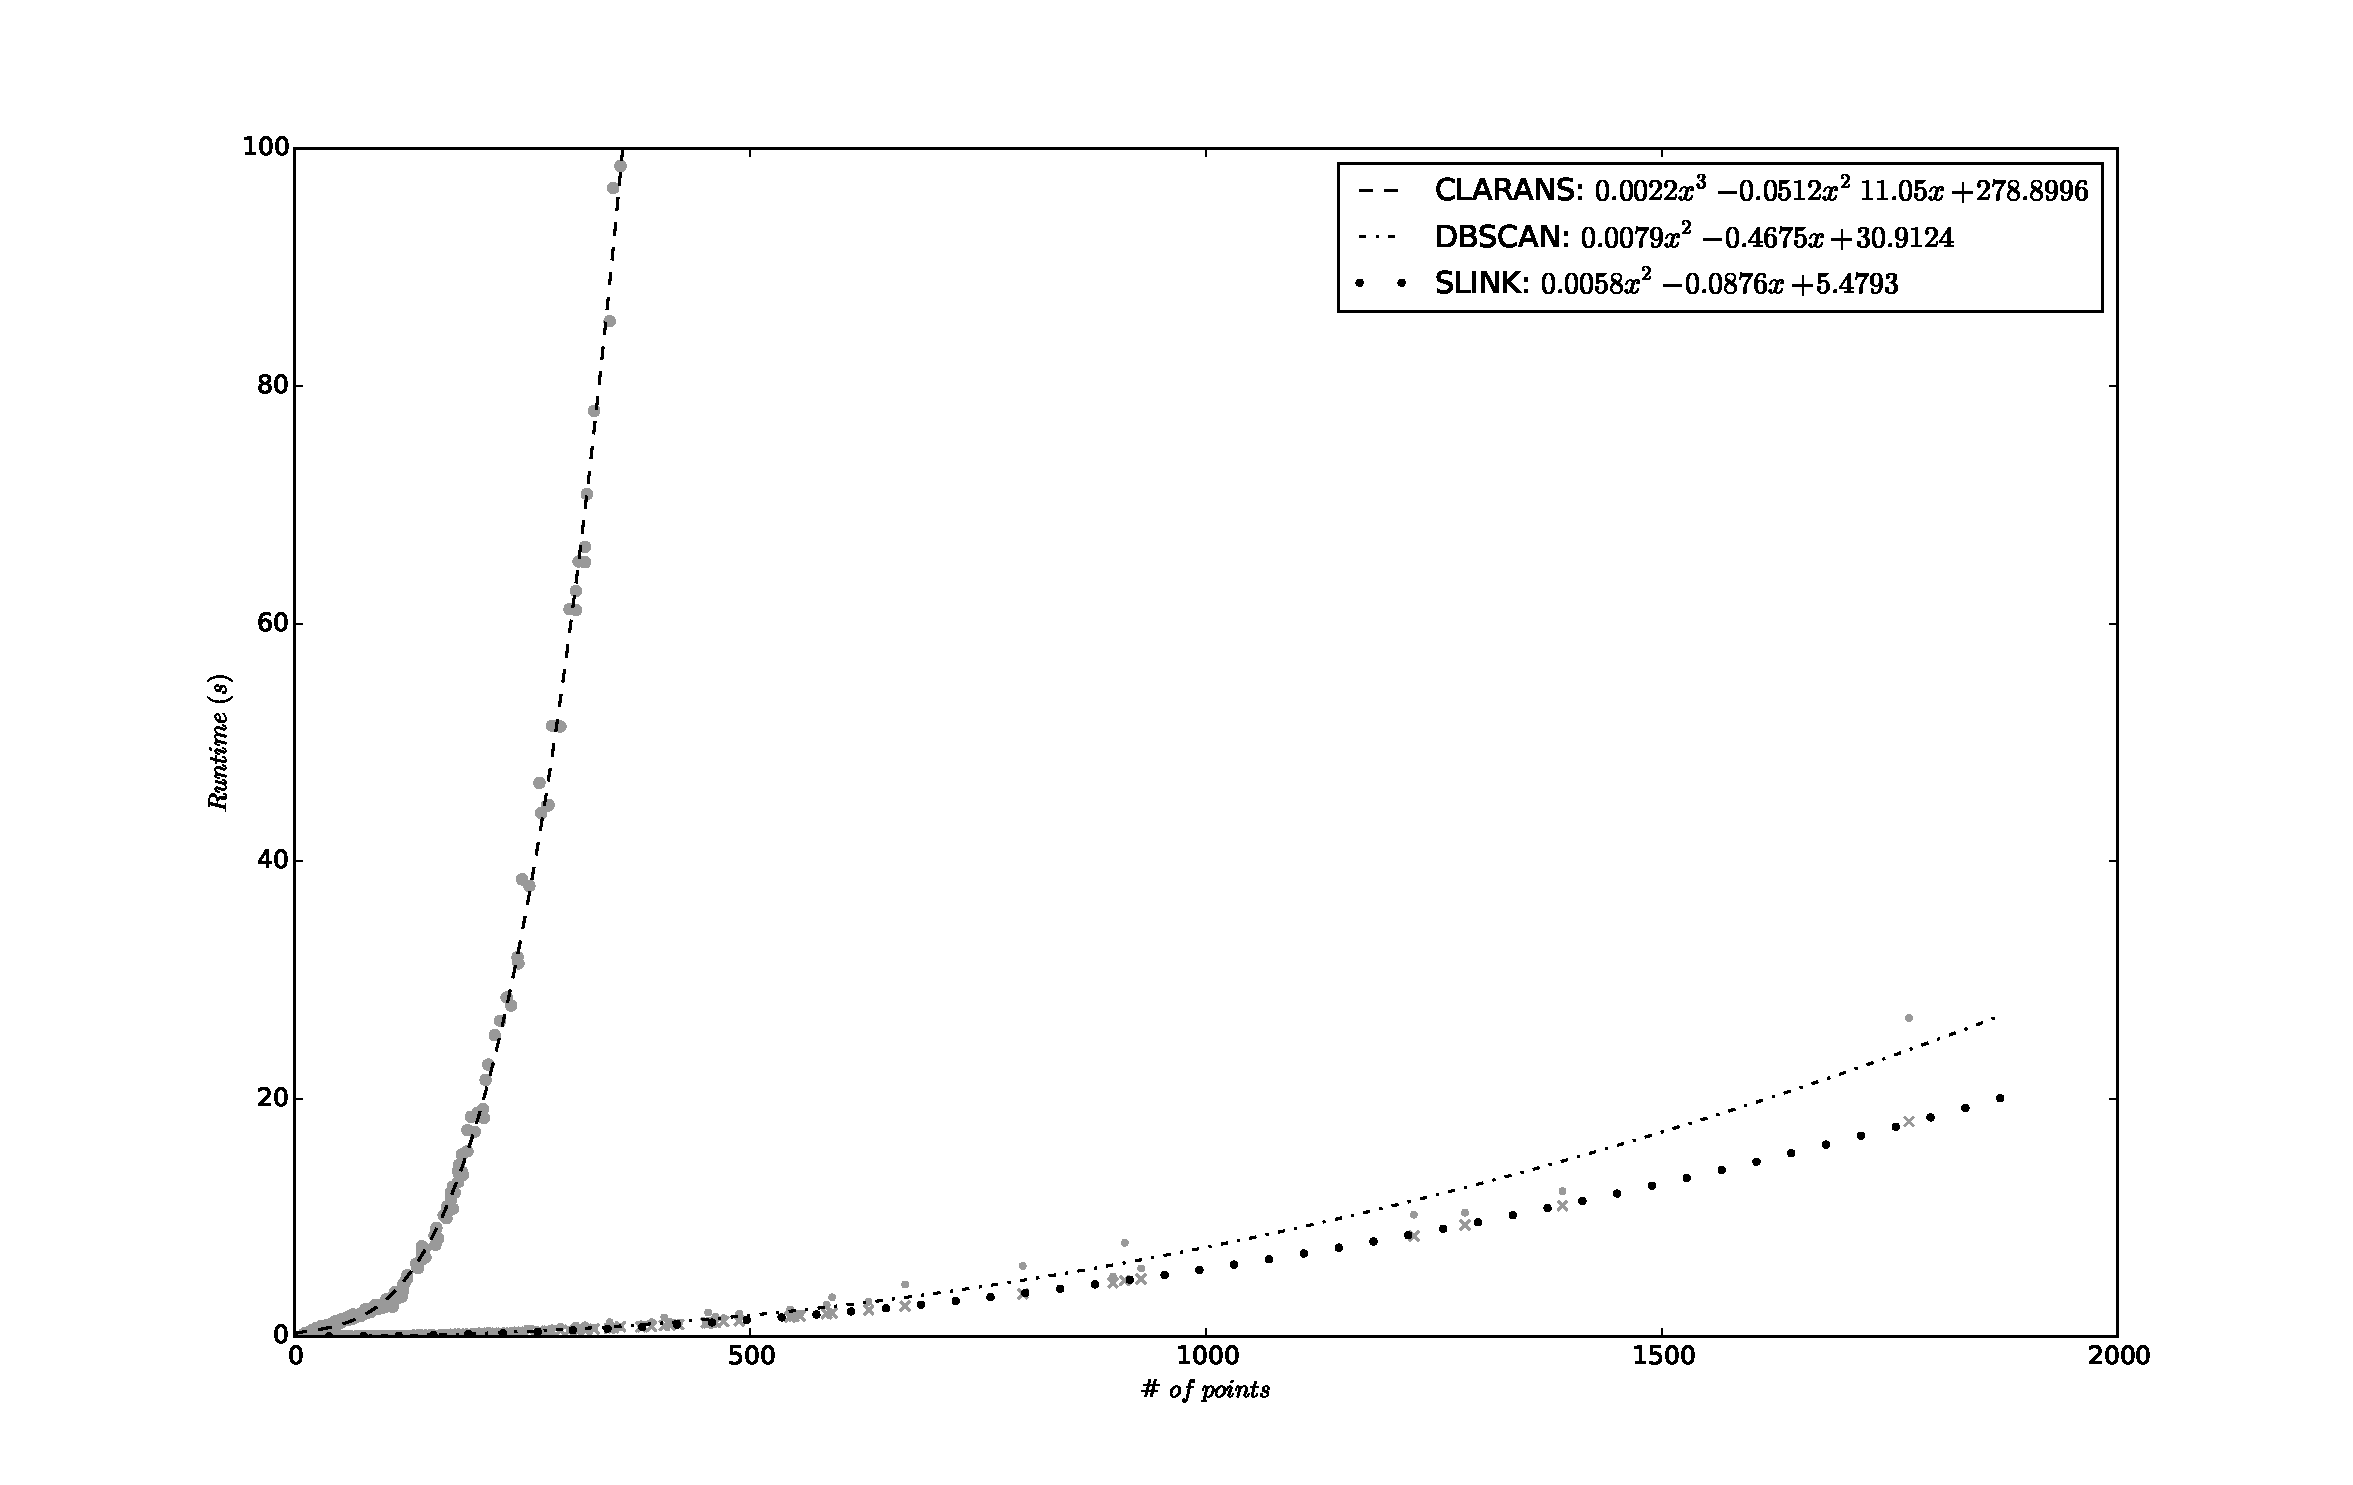
\includegraphics[width=0.9\textwidth]{plots/time_trendlines.pdf}
    \caption{Scatterplot of timestamps including trend lines.
    \label{fig:time-trendlines} }
\end{figure}

Using the polynomial fit for assessing \emph{trend lines} together with the 
observed data, coefficients for the polynomials are found yielding the trend 
lines as follows:
\begin{equation}
    \label{eq:trendline-equations}
    \begin{split}
        y_{CLARANS} &= 0.0022x^3 + 0.0512 x^2 +  11.05 x + 278.9 \\
        y_{DBSCAN}  &=           + 0.0079 x^2 + 0.4675 x +  30.9 \\
        y_{SLINK}   &=           + 0.0058 x^2 + 0.0876 x +   5.5
    \end{split}
\end{equation}
Plotting these along with the observed data is done in 
figure~\ref{fig:time-trendlines}, which makes the results seem feasible. 
It is likely to assume that these time complexities will hold for even 
larger numbers as well. 

It is worth noting that the region query algorithm used for DBSCAN is 
currently based on exhaustive search done in \ordo{n}, which leaves DBSCAN 
with a time complexity of \ordo{n^2}. A more rigid look up algorithm based 
on some R*-tree approach performing in \ordo{log(n)} should produce a 
somewhat faster result\footnote{
    Attempts were made at implementing this via RethinkDB:s spatial 
    queries, but unsuccessful as a mean of improving running time 
    efficiency loss. This is probable due to that RethinkDB is a database 
    focused on being distributed, yielding a time loss when querying the 
    database $n$ times. A faster approach was just to keep all data points 
    in memory. }.
An alternative to this if larger data sets are considered, is by either 
constructing some spatial index such as an R*-tree and inserting the data 
in it before performing spatial queries. \citeauthor{rtree-bulk-insert} 
did show that a bulk insert construction takes less than \ordo{n^2} 
time, and this spatial index implies a look up time of \ordo{ \log{n} }. 
Many databases already contain such indexes, and thus such queries can 
be done with a well considered database choice with simplicity \cite{rtree-bulk-insert}.

\subsection{Quality - Silhouettes}
Silhouettes are a measurement primarily for partitioning methods, and was 
originally developed with PAM and CLARA in mind by the authors 
\citeauthor{silhouettes} et al. An implicit assumption made, or a fact that is 
simply not considered, is that spatial points can be unassigned to clusters. 
The interpretation of Silhouettes here is simply not to treat these points 
and therefore, no evaluation of whether disregarding a point as noise is a 
good decision or not is taken into account.

Looking at figures~\ref{fig:clarans-silhouette}, \ref{fig:dbscan-silhouette} 
and~\ref{fig:slink-silhouette},
and taking the mean values depicted under each figure into account, it is 
clear that CLARANS produces the most qualitative clustering according to 
the criterion of maximizing the Silhouettes. This is expected, as the 
entire algorithms aim is to use the obtained Silhouette coefficients as 
feedback for how the algorithm is performing and which $k_{nat}$ to choose.

DBSCAN aims to eliminate bad clustering by regarding the entire observed 
Moment or data set as an activity. For the sake of being unbiased, a 
single detected cluster is awarded a Silhouette coefficient value of $0.5$,
which is why the algorithm produces that many clustering with the value of 
$0.5$. It has also the ability, unlike both CLARANS and SLINK, to disregard 
points as noise. Glancing at figure~\ref{fig:dbscan-vs-clarans} 
and~\ref{fig:dbscan-vs-slink} shows that DBSCAN generally produces few 
clusters given the set cluster parameters. This is desired, as we would not 
like a day to be divided into too many activities, and that a certain time 
should be spent at a certain location to deem it as an activity. 
Often for few data points, this setup yields a single cluster, disregardful 
of the Silhouette coefficient, which seems feasible as well as desirable.

SLINK produces poor clustering as well with regard to Silhouettes, partly 
because of the simple criterion on which the splitting is done. Unlike 
DBSCAN, it does not grant the ability to not use all the data points in the 
clustered result. During long, extended data sets right on the border of the 
limit value of breakpoints, a lot of clusters that are not very coherent will
be detected, leading to many clusters and to a poor clustering result. 

Taking one step back and evaluating the evaluation itself, it would seem like 
Silhouettes are not very suitable as a metric for comparing different 
clustering methods. However, it is one of few that is applicable 
at all regardless of which method is used, and therefore it is useful. One 
has to consider of course that the produced result is not easily interpretable, 
and requires prior knowledge about the algorithm being 
evaluated as well as insight in Silhouettes; how they are defined and some 
experience in how they behave when encountering different clustering. 
Given this, I argue that Silhouettes can be useful in a general 
manner and for a broader number of clustering applications, granted that 
one is familiar with the behaviour of Silhouettes. It serves as an aid to 
further evaluate why an algorithm performs as it does, and calls for 
another step of analysis. It is worth noting that a bad Silhouette score 
does not necessarily mean a bad clustering algorithm, it just means it is 
not optimized for this particular method.

\subsection{Produced Clusters}
Figure~\ref{fig:dbscan-vs-clarans}, \ref{fig:dbscan-vs-slink} 
and~\ref{fig:clarans-vs-slink} makes it very clear that different clustering
methods produce a different amount and different types of clusters. 

Generally, DBSCAN and CLARANS produce somewhat similar amount of clusters. 
This is due to that DBSCAN is not prone to produce many clusters given the
current clustering parameters, with $minPts$ set to $10\%$ of the data 
points, the absolute maximum number of clusters that is possible to obtain
is 10. In a similar manner, CLARANS is only able to produce at most 
$5$ clusters due to its limit set on the tests for $k_{nat}$. The produced
clusterings therefore does not differ very much in amount.

SLINK on the other hand tends to produce a lot more clusters in larger data
sets (as can be seen in both figure~\ref{fig:dbscan-vs-clarans} 
and~\ref{fig:clarans-vs-slink} where the number of clusters SLINK detects
diverges from the other algorithms more as the size of the data set increases). 
This is due to it's inability to disregard points as noise, while
bound to the same cutoff condition as DBSCANs $\epsilon$, yielding a lot
of small clusters containing a small number of points. Removing these would
be trivial in order to find remove noisy outliers with SLINK as well, but 
it would not serve any more comparison purposes than that.

\subsection{Large vs Small Data Sets}
Although CLARANS was specifically designed for working on larger data sets, 
both SLINK and DBSCAN outperforms CLARANS in the different sizes tested. 

As DBSCAN and CLARANS has an upper bound on the number of clusters that they
are able to detect in this instance as well, the results does not differ 
very much from the small data set. SLINK follows its previous trend 
with detecting even more clusters, since it is more flexible in its approach
on where to cut off its dendrogram into clusters.

\subsection{Method-specific qualities}
Different clustering methods have different qualities to take into account, 
both from a life-logging perspective, and with regard to finding different
types of clusters. 

CLARANS was built to maximize the Silhouette coefficient, and is useful for
finding clusters in very large data sets, especially large enough to not 
fit into the memory of the machine performing the clustering. Not keeping all
data points in memory would be a drawback for the other algorithms (granted 
that DBSCAN keeps its exhaustive search for nearby regions), but as it is 
randomized, clusters must be well-defined as well in order for it to locate 
them. This can be due to poor start-seed selections, meaning that the node 
chosen as a starting node is not very well spread out.
There exist methods for introducing starting seeds in partitioning
algorithms, usually with k-means being the target, but could applicable in 
this scenario as well. 
%When this is employed, the following results can
%be obtained following the same tests as above:

DBSCAN is easy to configure when working with activities and when following
equation~\ref{eq:minPts_eps_condition}, as one only needs to define 
how many data points are required for a series of samples to be considered
an activity. Disregarding outliers\footnote{
    An outlier is a data point that is distant from the other data points
    with regard to the distance function being used.
} is useful too, and making a qualitative
estimate of where the activity has taken place falls naturally. 
However, a decent knowledge about the size and characteristics of the 
assessed data set is necessary in order to get the desired result, and
clusters of varying densities are hard to distinct.  
Although the condition for selecting a good $\varepsilon$ and $minPts$ works
well with determining activities in a single cluster, it is not as 
accurate with higher number of data points and an expected higher number
of clusters. This since $minPts$ is set to contain a $10\%$ fraction of the total
points in the series to regard it as significant. A lower bound is also 
specified for this, and increasing DBCSANs performance of detecting more
clusters in bigger data sets could be accomplished by introducing an 
upper bound as well. 

SLINK is very customizable, as the splitting criterion defines which 
clusters are obtained. This would allow for more strict clustering
distinction, for instance by allowing time to a significant member in the 
distance function, and thus allowing finding of breakpoints in the time-line, 
and performing more strict clustering than DBSCAN.
SLINK also produces a hierarchical result. 
This hierarchical result is especially useful when multiple criteria 
need to be weighed in, and when allowing the result to be merged again or
split further without re-running the entire algorithm. 

\subsection{Desired Clusters}
From a life-logging point of view, there seem to be two different approaches
to what is a desired cluster to detect. 

One way, activity detection is of main interest and the output does not 
necessarily need to be in any specific form. What is desired is an estimate
of a location, time of stay and other similar data which will be used for 
classification or activity detection. It is more important that this produces
data that is neatly wrapped up and easy to present or use at a later step. 
This is the method used in the classification step of this thesis, when 
attempting to detect different activities. 

The alternative is that clustering in some hierarchy is required, where 
attributes are subordinated one another to perform division of data into 
smaller, ordered sets of data. This is what Narrative uses for dividing 
long series of images, into Moments (although, position or accelerometer
is currently not involved in this, only color data from images and timestamps 
are used for this clustering). Everything in this clustering is subordinated 
time, as Moments by Narratives definition is required to be coherent series 
of images. This calls for differently defined clusters, and thus differently
behaving clustering algorithms.

\section{Proof-of-Concept}
The proof-of-concept implementation conducted in this thesis adds components such
as clustering and classification to an already defined pipeline. The result of 
this implementation is presented earlier in this report, but the order of elements
in this already defined pipeline can be discussed. 

Long photo sequences are currently being divided into Moments solely based on 
timestamps and image analysis. It is at this point one would like to perform 
geo-spatial clustering if applicable, in order to get more natural Moments\footnote{
    The reason that no positional data is considered yet at this stage from 
    Narratives point of view is that no GPS points is available yet when the 
    \emph{Momentification} is done. This is produced later in the pipeline by 
    signal processing and by consulting servers for satellites positions. To 
    perform geo-spatial clustering in Narratives Momentification, this has to
    be addressed first. 
}. 
One might regard the existing implementation as a naive clustering algorithm, where 
introducing spatial data in the algorithm just increases the dimensionality, but
also the possibility of less artificial clusters. 


\section{Classification of Moments}

\subsection{Assessed Data Set}
As mentioned earlier, only employees were involved in the testing of the 
classification algorithm. It is feasible that employees of a company making
a certain life-logging device might utilize it another manner than the common 
user, which might have caused somewhat skewed results, but such that should
be sufficient for this thesis purposes.

\subsection{Possible Pitfalls}
As table~\ref{table:classification-values} witnesses of, the initial 
classification performs 
rather poorly, with each classification assignment except for the 
movement category only barely produced better 54\% correct 
approximations. There are many causes of this behaviour, and some 
being corrected led to  big improvement:

\begin{itemize}
\item The small sample for the algorithm to learn of was not sufficient, 
    and priors were not skewed enough to fit the model parameters to
    there correct location. This could have been prevented with a much
    bigger sample size. 
\item The sample for the learning algorithm were not diverse enough, and
    taken from a single user. Referencing 
    table~\ref{table:user-wise-mean-grade} it the mean value of users 
    assessments are widely varying. This can of course be a result of the
    users preferences while grading, but it also hints that the model 
    parameters are somewhat user-specific. For instance, a certain user 
    might move around more than another user while walking, therefore
    requiring somewhat different thresholds. Given this assumption, data
    from a small group of users will not reflect the entire population 
    of users, yielding skewed model parameters. 
\item The assigned probability distribution might not be suitable for the
    actual distribution, and thus the expert failed at the first attempt.
\end{itemize}

The model was simple and loosely defined upon assumptions, that might
prove more or less accurate. A model behaving incorrectly after many
learning attempts is probably an inaccurate model, but this should be
accommodated by updating ones model after observing its performance
in a true Bayesian manner.

The original intent of introducing such a model was for it to be 
simple and general enough to evaluate the method itself rather than
how this model would apply to Narratives employees and their Moments. 
Glancing ahead at the second attempt, it seems as the method holds.

\subsection{False Positives and Negatives}
Table~\ref{table:false-values-vs-grades} shows the correlation between
users grades for an entire activity classification, where the false 
negatives outweigh the number of false positives. Naturally, it seems 
more appealing for a user to receive a false negative rather than 
a false positive, implying that nothing special happened instead of 
saying something special happened while it did not. 

While the survey does not contain enough samples to statistically verify
this conclusively, it seems as a higher amount of false negatives is 
tolerated before lowering the grade of a classification, while false
positives are not tolerated at all. This backs our statements of false
positives being less appreciated. 

Given this information, one should focus on making an application that 
is less likely to produce a classification with greater semantic 
significance, as users seem more forgiving as towards missing out on 
classifications. As previously intended, assigned classes that are 
not semantically charged, which are assumed to be:
\begin{itemize}
    \item \emph{Alone} in the Social category.
    \item \emph{Off Hours} in the Working category.
    \item \emph{Stationary} in the Movement category.
    \item \emph{Indoors} in the Indoors category. 
\end{itemize}
should then not at all be shown to the end user, as they do not produce
enough value.

The scenario above applicable when the intention is to show the 
classifications to the end users. When the target instead is statistical
classification, for example in order for a company to determine the 
amount of activities its users engage in outdoors, these semantically 
charged notation is of less importance, as an overview of a whole group
is of greater interest than being correct in every individual case. 

\subsection{Second Attempt}

Analysis of the movement parameter is satisfactory, as it has three
possible outcomes and still manages to produce the best accuracy.

Relearning based on the new values allow a better fit for the observed
values, which are bound to be more diverse than samples from a single
user, as well as being a better quantity.

Looking at the results of the first attempt along with the number of
false positives and false negatives in table~\ref{table:classification-values} 
and table~\ref{table:false-values-before}, respectively, it is clear
that the categories \emph{Working} and \emph{Indoors} are not balanced.
Given that \emph{Working} depends on \emph{Indoors} (consulting 
figure~\ref{fig:bayes-network}), it seems logical in a first step to 
change \emph{Indoors}. By manually lowering the threshold of the 
model parameter (which was somewhat misplaced due to huge variance 
in the area-distribution), the results in table~\ref{table:classification-values} 
and table~\ref{table:false-values-before} were obtained.

Along with this, a relearning process is made where the percentages of 
the other assignments are somewhat improved, however not very 
significantly. Of course, this introduces a bias when the assessed data
is the same as the learned data, but given the sample size other tests
are not possible. This only illustrates the need of a larger data set 
for learning parameters, and the models influence in getting a faster
convergence towards correct classification.

This signals that a model error is present in the \emph{Indoors}-parameter,
and a model change should be done. In a Bayesian manner, preserving 
uncertainty is desired, and therefore introducing a second model
parameter denoting if the activity has any positional points could be
introduced. If this is the case, the area threshold is used, while 
otherwise, the original distribution of the \emph{Indoors} Bernoulli
variable is kept, thus preserving uncertainty.

\subsection{Iterative Process}

A way of looking at this attempt is simply as one stage of an iterative
process. In order for a sound model to develop with rigid model 
parameters several attempts seem to be required, and the first steps
of this process shows promise. It is also worth noting that the model
was initially predicted to not be too correct, as it was a simple 
version in order to evaluate the process and not the model. For a 
real-world implementation more analysis is definitely required in order
of creating more accurate predictions.

It has been shown that a learning step as well as a manual refinement of 
the model parameters result in a significant improvement. This is also
an example of how it is possible to go from a simple model producing 
mediocre results, to a more complex and targeted model towards more
specific problems.

\section{Big Data Ethics}

\subsection{What is Big Data?}

\begin{displayquote}
    ``Common definitions of the popular phrase for the phenomenon 
    “big data” are based on distinctions between the capabilities 
    of legacy database technologies and new data storage and 
    processing techniques and tools such as Hadoop clusters, 
    Bloom filters, and R data analysis tools. Big data is data too 
    big to be handled and analyzed by traditional database protocols
    such as SQL (which makes big data a term that  may evolve over 
    time; what is now big data may quite rapidly become small).''
    - \citeauthor{ethics-of-big-data}, author of 
    \citetitle{ethics-of-big-data} \cite{ethics-of-big-data}.
\end{displayquote}

What we particularly focus on in this thesis is just not the size,
but the applicability to make assumptions and draw conclusions based
on the observed user data. This is often the case for life-logging
devices, and cause for both use and abuse.

\subsection{Making Revenue}
Big data is a relatively new subject, or at least the extent of how it is used. 
Many companies are being able to make revenue on "free" services, which are free 
in the sense that the end user is the product. Mapping demographics and studying 
user behavior is becoming more and more a source of power for big data companies.
There are clearly different business models for the service providers, one being 
free-of-charge while collecting information about customers behaviours, the other 
being the classical approach of charging the end user for a service while not 
mining information about the user.

Simplified, it is two different payment methods for the users (while 
it might not be clear to the users themselves). The payment either comes
in the form of money, or utilizing your data, with various steps 
between. 

In any form - companies are not in the business of harming their customers,
so the customers are not the sole potential victims. As the amount of 
data increases, so does the need to protect the data and store it in a 
safe manner by the service provider. The more variate data that needs
to be stored in different ways, the more security holes need to be shut 
\cite{ethics-of-big-data}.

\subsection{An Ethics Code}

The need for an ethics code, or guidelines to follow when utilizing big data
computing is increasing with the number of companies engaging in the business.
\citeauthor{whats-up-with-big-data-ethics}:
\begin{displayquote}
    ``The problem is that our ability to reveal patterns and new 
    knowledge from previously unexamined troves of data is moving 
    faster than our current legal and ethical guidelines can manage.''
    - \citetitle{whats-up-with-big-data-ethics} 
    \cite{whats-up-with-big-data-ethics}.
\end{displayquote}

As \citeauthor{whats-up-with-big-data-ethics} states, the rapid development 
of Big Data services
has made law making as well as setting ethical guidelines fall behind, 
partly by lack of interest and the number of people involved, 
but even more so the unfamiliarity of the field. Venturing into a new 
area of technical implementations makes it hard to estimate what the 
different consequences might be. One can only try to predict the 
implications of Big Data services and to make decisions based on the
best judgment from there. If the guidelines are set too loose, the 
end users privacy will be endangered and will refer from using services
where they feel violated and exposed. Being too strict can instead
decrease quality of services.

\citeauthor{ethics-of-big-data} proposes 4 major questions that should 
be answered by such a code: \cite{ethics-of-big-data}
\begin{itemize}
    \item \textit{Identity} - What is the relationship between our 
        offline identity and our online identity?
    \item \textit{Privacy} - Who should control access to data?
    \item \textit{Ownership} - Who owns data, can rights to it be 
        transferred, and what are the obligations of people who 
        generate and use that data?
    \item \textit{Reputation} - How can we determine what data is 
        trustworthy? Whether about ourselves, others, or anything 
        else, big data exponentially increases the amount of 
        information and ways we can interact with it. This 
        phenomenon increases the complexity of managing how we are 
        perceived and judged.
\end{itemize}

It is important to realize that there can not be a single ethics 
code for all types of big data - as the services working with
big data and life-logging are too diverse, and restraining this 
in a too broad manner could drastically reduce very useful 
development of services. Utilizing a framework for companies to
build their ethical guidelines regarding Big Data on seems like
a productive way of streamlining the process, making company
policies more transparent and users can easier expect certain 
elements to be covered.

\subsection{Narratives Role}

Narrative is of a particular interest, given that the provided 
service can seem intrusive to some users.
This when capturing photographic information without the users active 
knowledge, but simply by wearing the Clip. This has been a factor in 
mind of the company since start-up, and measures have been taken in 
order to ensure the end users privacy.

The photos collected by the Clip is the users property, and by 
uploading it to Narratives paid cloud services no legal rights to 
the data is lost. The business model is the second one of the two 
mentioned above, meaning that the user demography data is not sold, 
and the intent of data collecting is to satisfy the end customer.

The Clip itself is also designed to look as a camera, in order to
make the surrounding aware of the fact in the same manner as when
taking a photograph with a handheld device.

From a legal perspective, the photographing by itself proves no 
complication, since the same laws dictate how a worn camera should be 
used as a hand-held camera; there is no distinction.

A necessity for a life-logging service like what Narrative provides is the
need to communicate it's values regarding big data ethics, ownership
of the data collected and similar. The ethics code need to be shared 
with the end users. In my own experience, when telling people about 
Narrative as a company or wearing the Clip, the most common questions
are those regarding privacy issues or ethical discussions. Even if 
the end users are not concerned, it seems like an important marketing 
opportunity to let everyone that uses the Clip to be a part of the 
community aware of a companies ethical code, and thus becoming an 
ambassador for the service they are using and the device that they are
wearing. 

This seems like wearables in general can profit from, as they are 
usually target for ethical discussion as life-logging devices, as well
as the users to some extent become walking billboards for the product. 
Doing so should also lead to a continuous discussion about this current
topic, leading to the development of general ethics codes that are
predictable and that does not seem alien to users.

\subsection{Is Privacy Broken?}
I would say no, it is not. But as more and more people utilize social
services and log their life digitally - privacy needs to be defined in
another manner. It is not possible to disappear off the grid as it 
was a couple of generations ago, and we leave digital breadcrumbs 
everywhere we go. But by making standardized, predictable ethical rules
that users are aware of, ownership of data and awareness might control
how we view our privacy in the future. 

It is especially important when utilizing Big Data to treat it as 
such, as Big Data. Anonymous content is rarely purely anonymous, as 
presenting a large number of factors even when concealing the name and
some other information about a person, it might still not be entirely
anonymous.

Information can also be deducted from observations, making it possible
to draw conclusion about a persons actions based on logged behaviour. 
Closely related to this is reputation, and particularly one about a 
person. Some decades ago, the reputation consisted (for a non-celebrity
person) of the manners one had in conversations with others, and 
possibly to the next row of individuals based on what those other people
said. Now it is possible for an individual to make an opinion about a 
person without ever meeting them, through social media. Yet alone,
computers can make their "opinion" about persons and draw conclusions 
based on these observations, making the service feel intimidating and 
as a breach of privacy.

Deducting wrongful information can be just as bad, by implying that 
a user has done something or is interested in something that they in 
turn find offensive.

This calls for a question about the degree of ownership and to what 
extent we own our own traits, both in the offline world and the 
online, that enable services and people to make second hand deductions 
about private matters about us \cite{ethics-of-big-data}.


\chapter{Conclusion}
\label{ch:conclusion}
%%%%%%%%%%%%%%%%%%%%%%%%%%%%%%%%%%%%%%%%%%%% 80 line marker %%%%%%%%%%%%%%%
Clustering and classification of data are two closely related subjects, 
that can utilize methodologies that diverge more or less. In this thesis 
various clustering methods consisting of representatives from different
algorithm families have been evaluated based on their suitability for 
life-logging devices, and in particular, the Narrative Clip. Bayesian 
inference has then been used for classification of the activities detected 
by the clustering algorithms, allowing labels to be attached to each 
activity. 

%CLUSTERING
Comparing produced clusters and expecting exact similarity between different
algorithms is not a good approach. As mentioned early in this report, 
there is no universal definition of a cluster and therefore no universal 
clustering algorithm. Taking this into account, it is a better approach to
venture beyond strict similarity in produced clustering, and compare other 
metrics, such as number of detected cluster, performance, Silhouettes and so
on. But the most important examination point is the cluster algorithms 
characteristics and abilities, basically what it was meant to do.

CLARANS was the representative from the category of partitioning clustering 
methods. While partitioning methods in general are easy to implement and to 
understand, they have drawbacks that are significant, embodied by the results 
of CLARANS. The performance is poor due to the knowledge about the number of 
clusters being a prerequisite, requiring several runs of the algorithm and 
evaluating the result. Choosing the clustering parameters for CLARANS is 
unintuitive, since it is based on random search of a solution graph, and may 
find different solutions to the same problem, with varying quality. Bearing 
all this in mind, partitioning methods and particularly CLARANS seem 
inappropriate for life-logging applications, as the knowledge of the number
of clusters that exist on beforehand is a luxury that we usually do not have.
The execution time necessary to find the appropriate number of clusters
make usage of this not feasible, as it is implied by being automatic, that
this should be used in real-time.

DBSCAN performs well in run time, both for small and for large sets of data 
points. The choice of clustering parameters affects the amount of clusters, 
and the type of clusters one is willing to find. In the tested configuration, 
the algorithm seems most suitable for finding a little bit more fuzzy clusters
containing a rough position and outline, but not necessarily sorted by time. 
This is useful in activity detection, where a more neatly presented and 
approximated cluster is more appreciated and easier to use for a 
classification algorithm.

SLINK runs slightly faster than DBSCAN in the considered test cases, and 
is more flexible in the way it produces clusters. This allows for clusters to 
be cutoffs in a time-line, which is suitable for Moment detection, where a more 
strict definition of a cluster is required. The same could be said for several 
other applications, where time or other factors need to be sorted in first hand 
to produce clusters. 

This yields two different areas where DBSCAN and SLINK are applicable, in
activity detection and in Moment division, respectively. Life-logging is in 
its essence full of data mining problems that needs to be solved, and utilizing
these or other algorithms on other problems is very likely, but examining the
entire life-logging area is not within the scope of this article. The conclusion
is just that these two applications is appropriate for these two problems.

Silhouettes are not a simple metric to use when evaluating different types of
clustering algorithm, due to the different definitions of a cluster and the
varying output from the algorithm. Although not being able to simply compare
numbers in order of determining quality of a clustering algorithms produced
output, Silhouettes could still be useful to examine how an algorithm behaves,
and why the produced result look the way they do. 

% CLASSIFICATION

When it comes to classification, the results seem somewhat individualized, 
both when it comes to what users think is important regarding assigned classes, 
and especially the model parameters determining the classes. 

From a simple model promising results were achieved, when allowing an iterative 
approach in a Bayesian manner. After all, there is nothing more Bayesian than 
updating beliefs after witnessing evidence! The used model was made simple to 
make it easy to perform an update step, thus showing that this improved the 
quality of the output significantly. 

Model changes, even seemingly small, are more powerful than Bayesian learning 
via learning data and model fitting. In this thesis, a rather small set of
learning data was used, due to both time and resource constraints. This caused
parameters not to be set too robustly, especially parameters with great 
variance suffered by not being able to converge fast enough. From this, we 
learn that studying the parameter values is important as well after learning
to be confident in a model.

\section{Further Research}
This report presents an overview for clustering and classification, and 
discusses suitability of some methods as well as identifying pitfalls. 
Life-logging in its essence is about in an automated fashion storing 
activities for the monitored object, in Narrative's case, the end user. 
This usually results in vast amounts of data that needs to be processed 
in order of retrieving summaries or more qualitative data. Everything 
that automates and improves the process of automation is interesting to
this area, as it improves the quality of service. 

Investigating model learning and Bayesian network learning would be an 
interesting next step for taking the automated process one step further.

\subsubsection{Phone coupling}
As of now, the GPS data obtained by the Clip is rather sporadic, and
not very accurate. Phones today are 
however better at positioning, and utilizes other methods such as 
WiFi for a better positioning approximation \cite{iphone-wifi}.

It does also seem likely that a user carries his or her phone while 
wearing the Clip, and making use of this data should lead to a 
more quantitative and qualitative positional data, in its turn 
simplifying and making the result of clustering more useful to the
end users. Examining what more quantitative and qualitative data 
produces from a starting point is appealing.

\subsubsection{Momentification}
Introducing other clustering factors than geo-spatial data and 
time labels seem feasible as well, and especially monitoring 
statistical breakpoints in sensor-data proves especially promising. 
To introduce this either as another dimension in the clustering data, 
or correlation the detected geo-spatial clusters with the proposed 
clusters based on statistical breakpoints.

\subsubsection{Dynamic Learning}
An interesting approach for extending the classification would be to
introduce dynamic learning for the classification algorithm. As is 
stated previously, the model parameters seem somewhat individualized, 
and making these depend on user feedback. Such feedback can both 
come in the form of explicit evaluations on a web-based service, or 
by observing user behaviour and assessing whether certain actions are
a positive or a negative stimuli.

\printbibliography

\begin{appendices}

\addtocontents{toc}{\setcounter{tocdepth}{0}}

\chapter{Clustering Theory}
\label{app:clustering-algorithms-theory}

%%%%%%%%%%%%%%%%%%%%%%%%%%%%%%%%%%%%%%%%%%%% 80 line marker %%%%%%%%%%%%%%%
This presents the algorithms used in the paper more in-depth, and presents
the implementation used during test (to some extent). Python is used as 
implementation language due to its expressibility, and in order to get 
somewhat more of a standard than just pseudo-code.

Each example starts with an overview of the suggested pros and cons presented
in each article introducing the algorithms. 

The code examples have been slightly altered for readability purposes, and 
functions used have been omitted for brevity. The intent is to show the
core functionality of each algorithm.

\newpage

\section{CLARANS}

\emph{CLARANS - Clustering Large Applications based on RANdomized Search)}
is a partitioning clustering algorithm which divides the given data set 
into $ k_{nat} $ clusters, each cluster represented by a medoid point. 

CLARANS can essentially be viewed as a graph search, where each node in 
the graph represents a distinct selection of medoid representatives of
each cluster. Each node in the graph is considered to have vertexes to 
all nodes which differ in the selection of mediod nodes by one. The graph
search is randomized, and thus CLARANS is not deterministic, meaning that
inputting the same problem twice can lead to different solutions.

As all clustering algorithms, CLARANS needs parameters to specify the way
the clustering is performed. $maxneighbour$ determines how many random
neighbours of a solution node should be examined and $numlocal$ decides
how many local minima should be tried out before halting. $k$ could also
be considered as a parameter for the algorithm, and dexides how many
clusters to find. The solution for ignoring $k$ as a parameter, 
suggested by \citeauthor{CLARANS}, is to run the algorithm several times
with different $k$ and examine the result of each turn, in order of 
finding the $k$ that will be used as $k_{nat}$. 

Given this, it is obvious that the size size of this graph $ G $ is 
\begin{equation}
    \label{eq:clarans_size}
    \mid G_{v,k} \mid = \binom{n}{k}
\end{equation}
and that each the degree
\begin{equation}
    \label{eq:clarans_dimens}
    deg(v) = k(n-k)
\end{equation}
Therefore, when presented with equation~\ref{eq:clarans_dimens}, it is 
clear that letting $maxneighbour$ exceed this value is inefficient, 
since this means re-examining nodes that has already been deemed unfit.

The algorithm is in it's original paper as follows
\begin{enumerate}
    \item Initialize parameters $numlocal$ and $maxneighbour$.
          Initialize $i$ to 1 and $mincost$ to a large number.
    \item Set $current$ to an arbitrary node in $ G_{n,k} $.
    \item Set $j$ to 1.
    \item Consider a random neighbour S of $current$, and based on
          [equation 5], calculate the cost defferential of the two nodes.
    \item If $S$ has a lower cost, set $current$ to $S$
          and go to step (3).
    \item Otherwise, increment $j$ by 1. If $j \leq maxneighbour$, goto
          step (4).
    \item Otherwise, when $j > maxneighbour$ compare the cost of 
          $current$ with $mincost$. If the former is less than $mincost$,
          set $mincost$ to the cost of $current$ and set $bestnode$
          to $current$.
    \item Increment $i$ by 1. If $i > numlocal$, output $bestnode$ and halt.
          Otherwise go to step (2).
\end{enumerate}

\newpage

\subsection{Algorithm}

\begin{python}
def CLARANS(S, k_nat, numlocal, maxneighbour):
    min_cost    = float('inf')
    best_nodes  = None
    
    for i in range(numlocal):
        # Random selection of a starting node.
        random.shuffle(S)
        current = S[ -k_nat:]
        points  = S[:-k_nat]
        
        current_cost = self.cost(current, points)
        
        j = 1
        s_p = points
        while j <= maxneighbour:
            # Select a random neighbour
            nbr = current
            s_p = [s.pop(random.randrange(len(nbr)))] + s_p
            nbr.append(s_p.pop())
            
            if self.cost(s, s_p) < current_cost:
                current, points = (s, s_p)
                current_cost = cost(current, points)
                j = 1 
            else: 
                j += 1
        
        if current_cost < min_cost:
            min_cost    = current_cost
            best_nodes  = current
            
    return best_nodes
\end{python}

\newpage

\section{SLINK}

SLINK is an hierarchical algorithm which in practice does not actually
perform any clustering, but structures the data into a dendrogram using
a specific pointer notation. This pointer notation is what makes SLINK's
improved run-time \ordo{n^2} possible, as an improvement over 
traditional hierarchical clustering algorithms which runs in \ordo{n^3}.

SLINK is an aggleromative method, constructing the clusters bottom up, 
with the starting point of each datum in the clustered data set to 
be its own cluster, and continuing to combine clusters until all data
is in the same cluster. The combining of clusters is done using 
Single Linkage criterion \footnote{
    Single Linkage (or nearest-neighbour) is a measurement of the 
    similarity of two clusters defined by the two most similar members. 
    Alternatives to this is Complete Linkage, which compares the two 
    most dissimilar members, and Average Linkage.
}, which is also where the algorithm gets its name. 

This algorithm is proven to be optimally efficient in hierarchical 
clustering. \cite{SLINK}

\subsection{Pointer notation}
As mentioned above, what makes SLINK significantly faster than classical, 
naive implementations of clustering algorithms is its utilization of a 
pointer notation. The pointer notation used in the SLINK is defined as 
follows:

Lets introduce two functions that are defined on the set of indexes for
the $N$ data objects to be clustered:

\begin{definition}[Pointer definitions for SLINK]
\label{definition:pointer-representation}
    Let 
    $$
        \pi : 1,...,N \rightarrow 1,...N
    $$
    so that $\pi(N) = N$, and let 
    $$
        \lambda : 1,...,N \rightarrow [0, \infty]
    $$
    so that $\lambda(N) = \inf$, and  
    $$
        \pi(i) > i \quad \lambda(\pi(i)) > \lambda(i) \quad ,i < N
    $$
\end{definition}

The interpretation of $\pi$ and $\lambda$ respectively should be that
$\pi(i)$ is the last object in the cluster which $i$ joins, and $\lambda(i)$
is the distance to that cluster. 

\subsubsection{Example}
This is an example of where SLINK has already been performed, and transformed
a given data-set into a dendrogram. 
Table~\ref{table:pointer-representation-example} shows the pointers value, while
figure~\ref{fig:pointer-representation} displays the corresponding dendrogram 
interpretation. 

\begin{table}
    \centering
    {\begin{tabular}{ | l | c c c c c c c c c c | }
        \hline
        Index     & 0    & 1    & 2    & 3    & 4    & 5    & 6    & 7    & 8    & 9 \\
        \hline
        $\pi$     & 6    & 3    & 3    & 5    & 9    & 9    & 8    & 9    & 9    & 9 \\
        $\lambda$ & 1.94 & 0.42 & 0.83 & 1.56 & 3.12 & 10.9 & 1.63 & 1.20 & 4.99 & $\infty$ \\
        \hline
    \end{tabular}}
    \caption{Pointer representation example \cite{pointer-representation}.} 
    \label{table:pointer-representation-example}
\end{table}

\begin{figure}[ht]
    \centering
    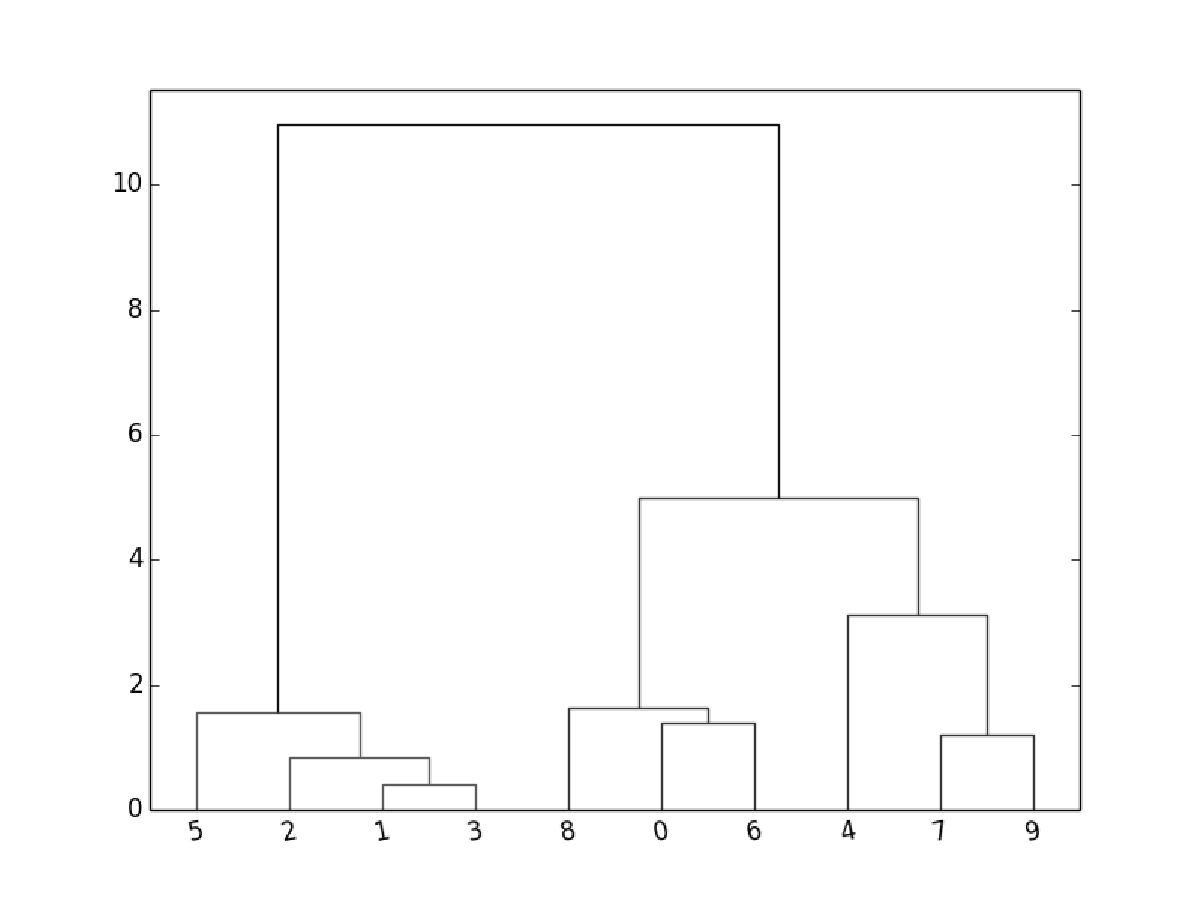
\includegraphics[width=0.8\textwidth]{images/pointer_representation.pdf}
    \caption{An example of the pointer representation of SLINK
        \cite{pointer-representation}. \label{fig:pointer-representation} }
\end{figure}

\newpage

\subsection{Algorithm}

The algorithm takes some data set $S$ with $n$ data points in it, and
utilizes three arrays of length $n$ to store the pointer representation.
These are called $\Pi. \Lambda, M$.

\begin{enumerate}
    \item Set $\Pi(n+1)$ to $n+1$, $\Lambda(n+1)$ to $\infty$.
    \item Set $M(i)$ to $d(i, n+1)$ for $i=1,...,n$.
    \item For $i$ increasing from $1$ to $n$ \\
        if $\Lambda(i) \geq M(i)$ \\
            set $M(\Pi(i))$ to $ min\{M(\Pi(i)), \Lambda(i)\}$ \\
            set $\Lambda(i)$ to $M(i)$ \\
            set $\Pi(i)$ to $n+1$ \\
        else \\
            set $M(\Pi(i))$ to $ min\{M(\Pi(i)), M(i)\}$ 
    \item For $i$ increasing from $1$ to $n$ \\\
        if $\Lambda(i) \geq \Lambda(\Pi(i))$ \\
            set $\Pi(1)$ to $n+1$.
\end{enumerate}

\begin{python}
def SLINK(S):
    points  = S.get_points()
    n       = len(points)
    
    pi, _lambda, M = [0]*n, [float("inf")]*n, [None]*n
    
    for i in range(1, n):
        pi[i] = i
        
        for j in range(i):
            M[j] = distance(points[i], points[j])
        
        for j in range(i):
            if _lambda[j] >= M[j]:
                M[pi[j]] = min(M[pi[j]], _lambda[pi[j]])
                _lambda[j] = M[j]
                pi[j] = i
            else:
                M[pi[j]] = min(M[pi[j]], M[j])
        
        for j in range(i):
            if _lambda[j] >= _lambda[pi[j]]:
                pi[j] = i
        
    return (_lambda, pi)
\end{python}

\newpage

\section{DBSCAN}

\emph{DBSCAN - Density Based Spatial Clustering of Applications with 
Noise} is an algorithm proposed by \citeauthor{DBSCAN} in 
\citeyear{DBSCAN}. It relies heavily on 6 definitions, which provides an 
outline for the algorithm.

Two input parameters are required, $\varepsilon$ which defines the 
neighborhood size of a point (see \ref{definition:eps-neigborhood}), and
$MinPts$ that determines the minimum number of points in a cluster.
These together define a notation of cluster density.

\subsection{Definitions}

\begin{definition}[$\varepsilon$-neighborhood of a point]
\label{definition:eps-neigborhood}
    The $\varepsilon$-neighborhood of a point $p$, denoted by
    $N_\varepsilon(p)$, is defined by 
    $$
        N_\varepsilon(p) = \{ q \in D | dist(p,q) \leq \varepsilon \}
    $$
\end{definition}

\begin{definition}[Directly Density-Reachable]
\label{definition:directly-density-reachable}
    A point $p$ is directly density-reachable from a point $q$ with 
    regard to $\varepsilon$ and $MinPts$ if
    \begin{enumerate}
      \item $ p \in N_\varepsilon(q) $ and
      \item $ |N_\varepsilon(q)| \geq MinPts $ (core point condition).
    \end{enumerate}
\end{definition}

\begin{definition}[Density-Reachable]
\label{definition:density-reachable}
    A point $p$ is density-reachable from a point $q$ with regard to
    $\varepsilon$ and $MinPts$ if there is a chain of points 
    $p_1, p_2, \ldots, p_n$, $p_1=q$, $p_n=p$ such that $p_{i+1}$ is
    directly density reachable from $p_i$.
\end{definition}

\begin{definition}[Density-Connected]
\label{definition:density-connected}
    A point $p$ is density-connected to a point $q$ with regard to
    $\varepsilon$ and $MinPts$ if there is a point $o$ such that both
    $p$ and $q$ are density-reachable from $o$ with regard to 
    $\varepsilon$ and $MinPts$.
\end{definition}

\begin{definition}[Cluster]
\label{definition:dbscan-cluster}
    Let $D$ be a database of points. A clustrer $C$ with regard to
    $\varepsilon$ and $MinPts$ is a non-empty subset of $D$ satisfying
    the following conditions:
    \begin{enumerate}
        \item $\forall p, q$: if $p \in C$ and $q$ is density-reachable
        from $p$ with regard to $\varepsilon$ and $MinPts$, then
        $q \in C$: Maximality)
        \item $\forall p, q \in C$: $p$ is density-connected to $q$ 
        with regard to $\varepsilon$ and $MinPts$.
    \end{enumerate}
\end{definition}

\begin{definition}[Noise]
\label{definition:dbscan-noise}
    Let $C_1,...C_k$ be the clusters of the database $D$ with regard
    to parameters $\varepsilon_i$ and $MinPts_i$, $i=1,...k$. Then we
    define the noise as the st of points in the database $D$ not 
    belonging to any cluster $C_i$, i.e. 
    $noise = \{ p \in D | \forall i: p \not\in C_i \}$ 
\end{definition}

\newpage

\subsection{Algorithm}
\begin{python}
def DBSCAN(S, eps, minPts)
	# The initial set of points S is initialized  
	# with clusterID set to UNCLASSIFIED.
	clusterID = nextId(NOISE)
	
	for point in S
		if point.clusterId == UNCLASSIFIED
			if expandCluster(S, point, clusterID, eps, minPts)
				clusterID = nextID(clusterID)

def expandCluster(S, point, clusterID, eps, minPts)
	seeds = S.regionQuery(point, eps)
	
	# Core point criterion not fulfilled for point, 
	# so this is temporary regarded as noise.
	if len(seeds) < minPts
		point.clusterID = NOISE
		return False
	
	for p in seeds
	    p.clusterID = clusterID
	
	seeds.remove(point)
	
	while not seeds.empty()
		current = seeds.pop()
		result = s.regionQuery(current, eps)
	
		if len(result) >= MinPts
			for p in result
				if p.clusterID in [UNCLASSIFIED, NOISE]
					if p.clusterID = UNCLASSIFIED
						seeds.append(p)
					p.clusterID = clusterID
	return True
\end{python}

\chapter{Larger figures}
\label{app:larger-figures}

\begin{sidewaysfigure}
    \centering
    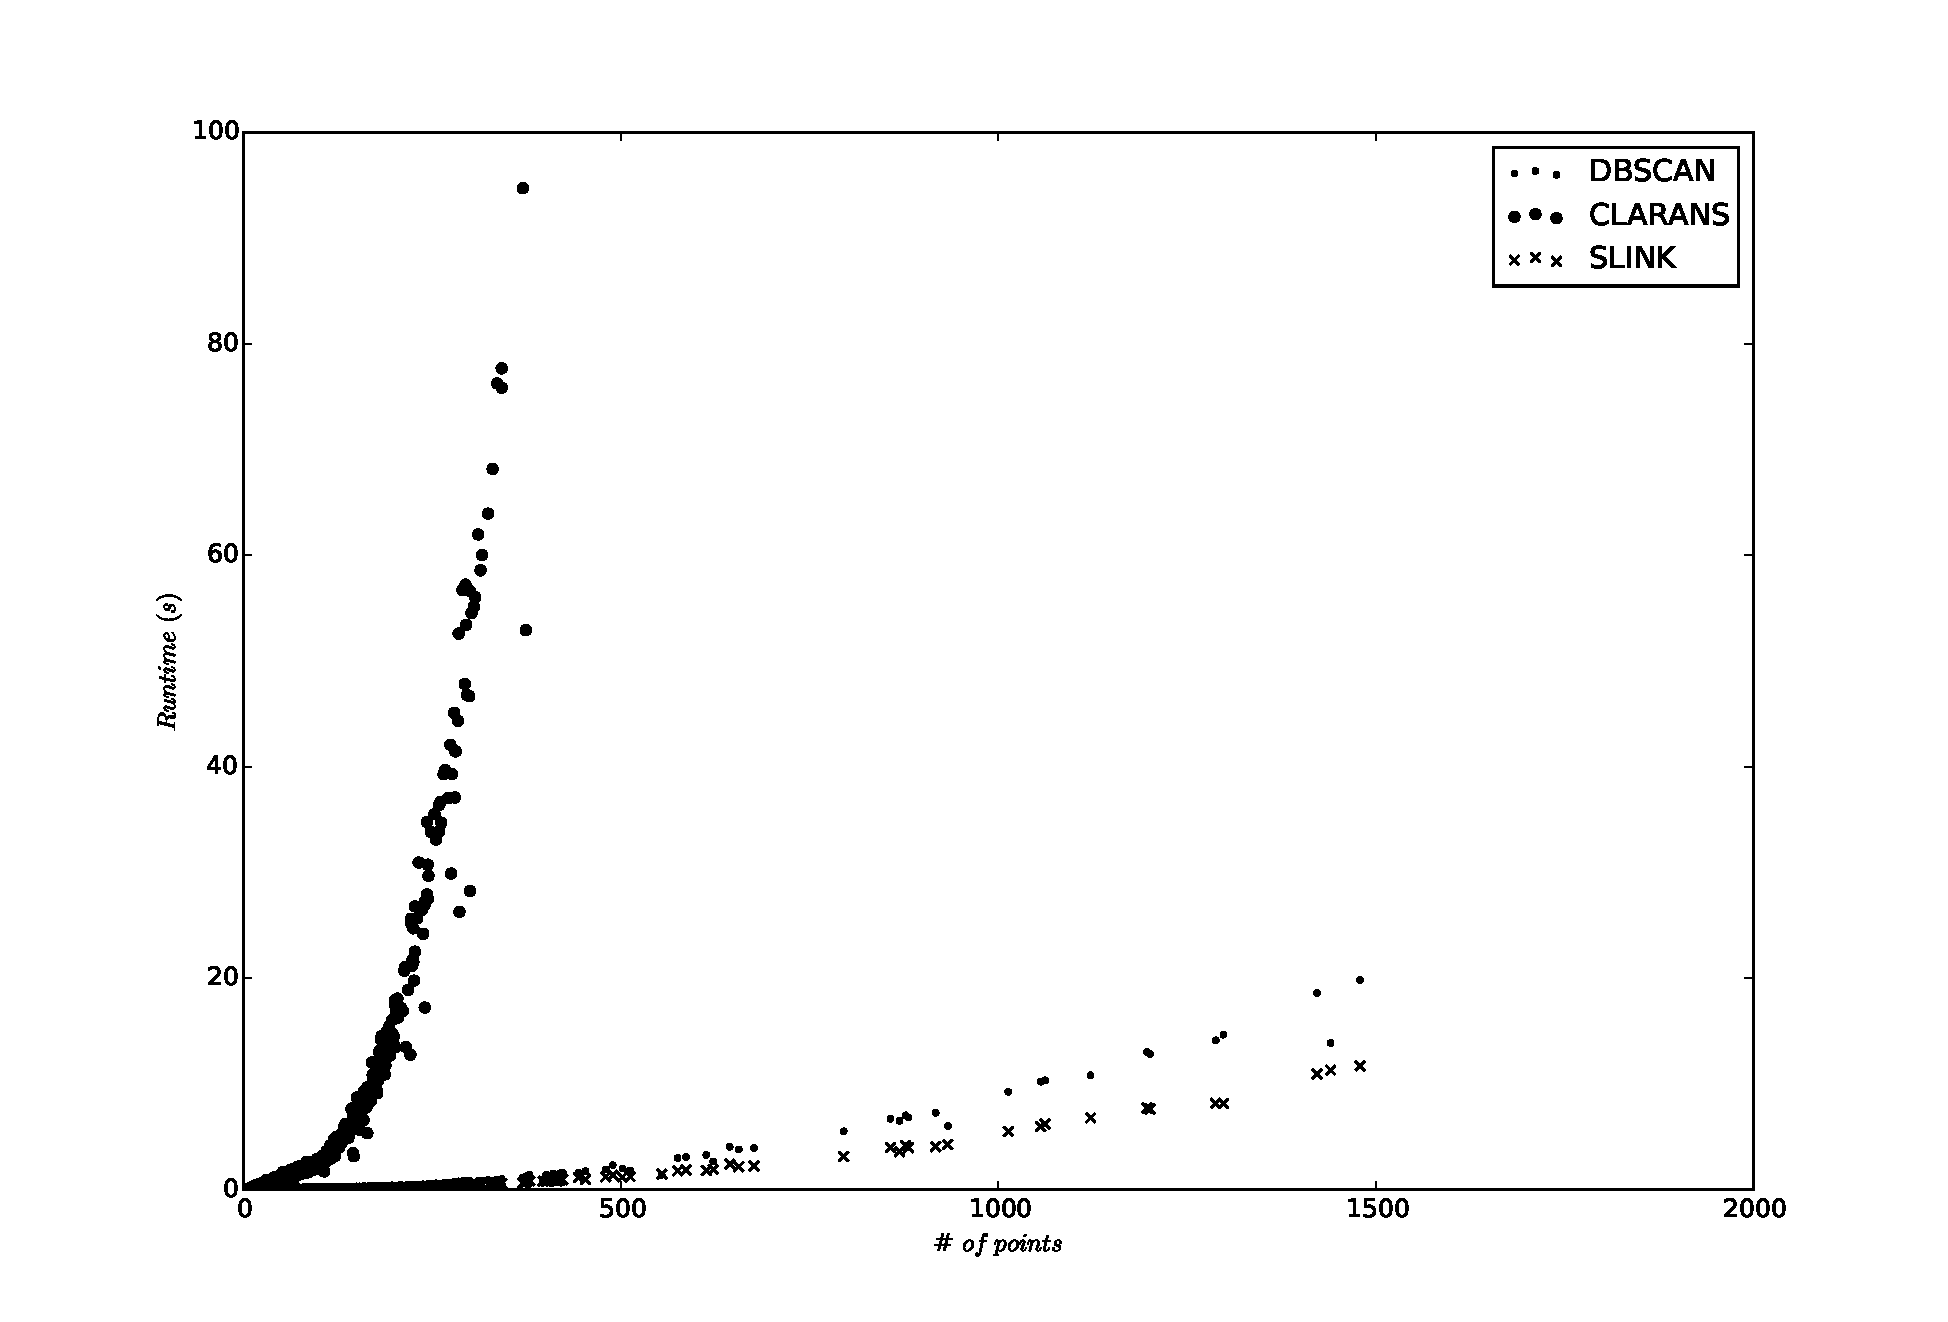
\includegraphics[width=0.9\textwidth]{plots/moment_runtime_scatter.pdf}
    \repeatcaption{fig:moment-runtime-scatter}{
        Run-time for clustering algorithms over Moments, by number of points in the moment.}
\end{sidewaysfigure}

\begin{sidewaysfigure}
    \centering
    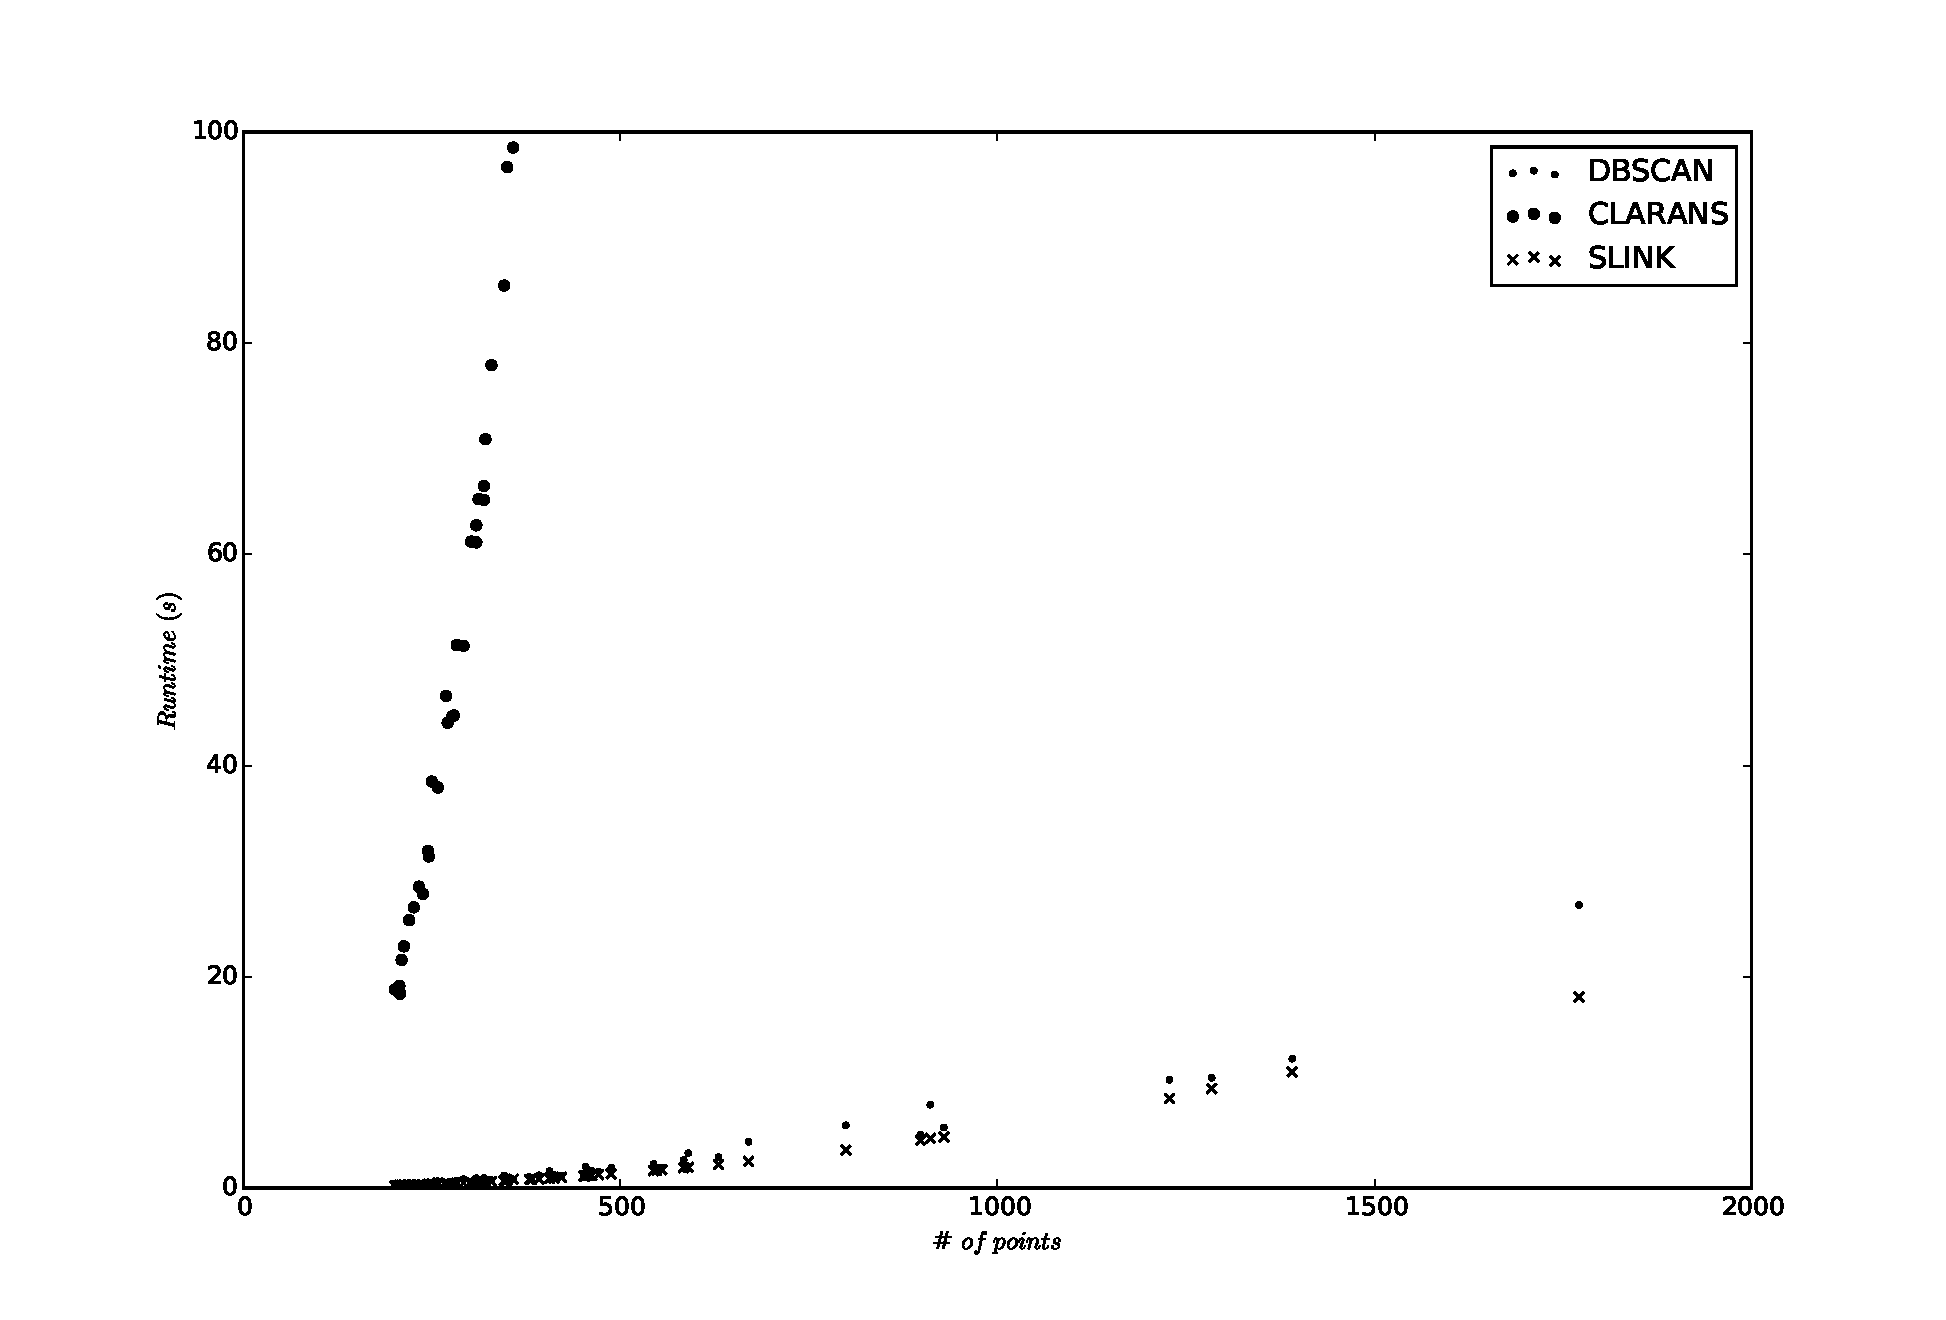
\includegraphics[width=0.7\textwidth]{plots/days_runtime_scatter.pdf}
    \repeatcaption{fig:day-runtime-scatter}
    {Run-time for clustering algorithms over users days, by number of points on the day. }
\end{sidewaysfigure}

\begin{sidewaysfigure}
    \centering
    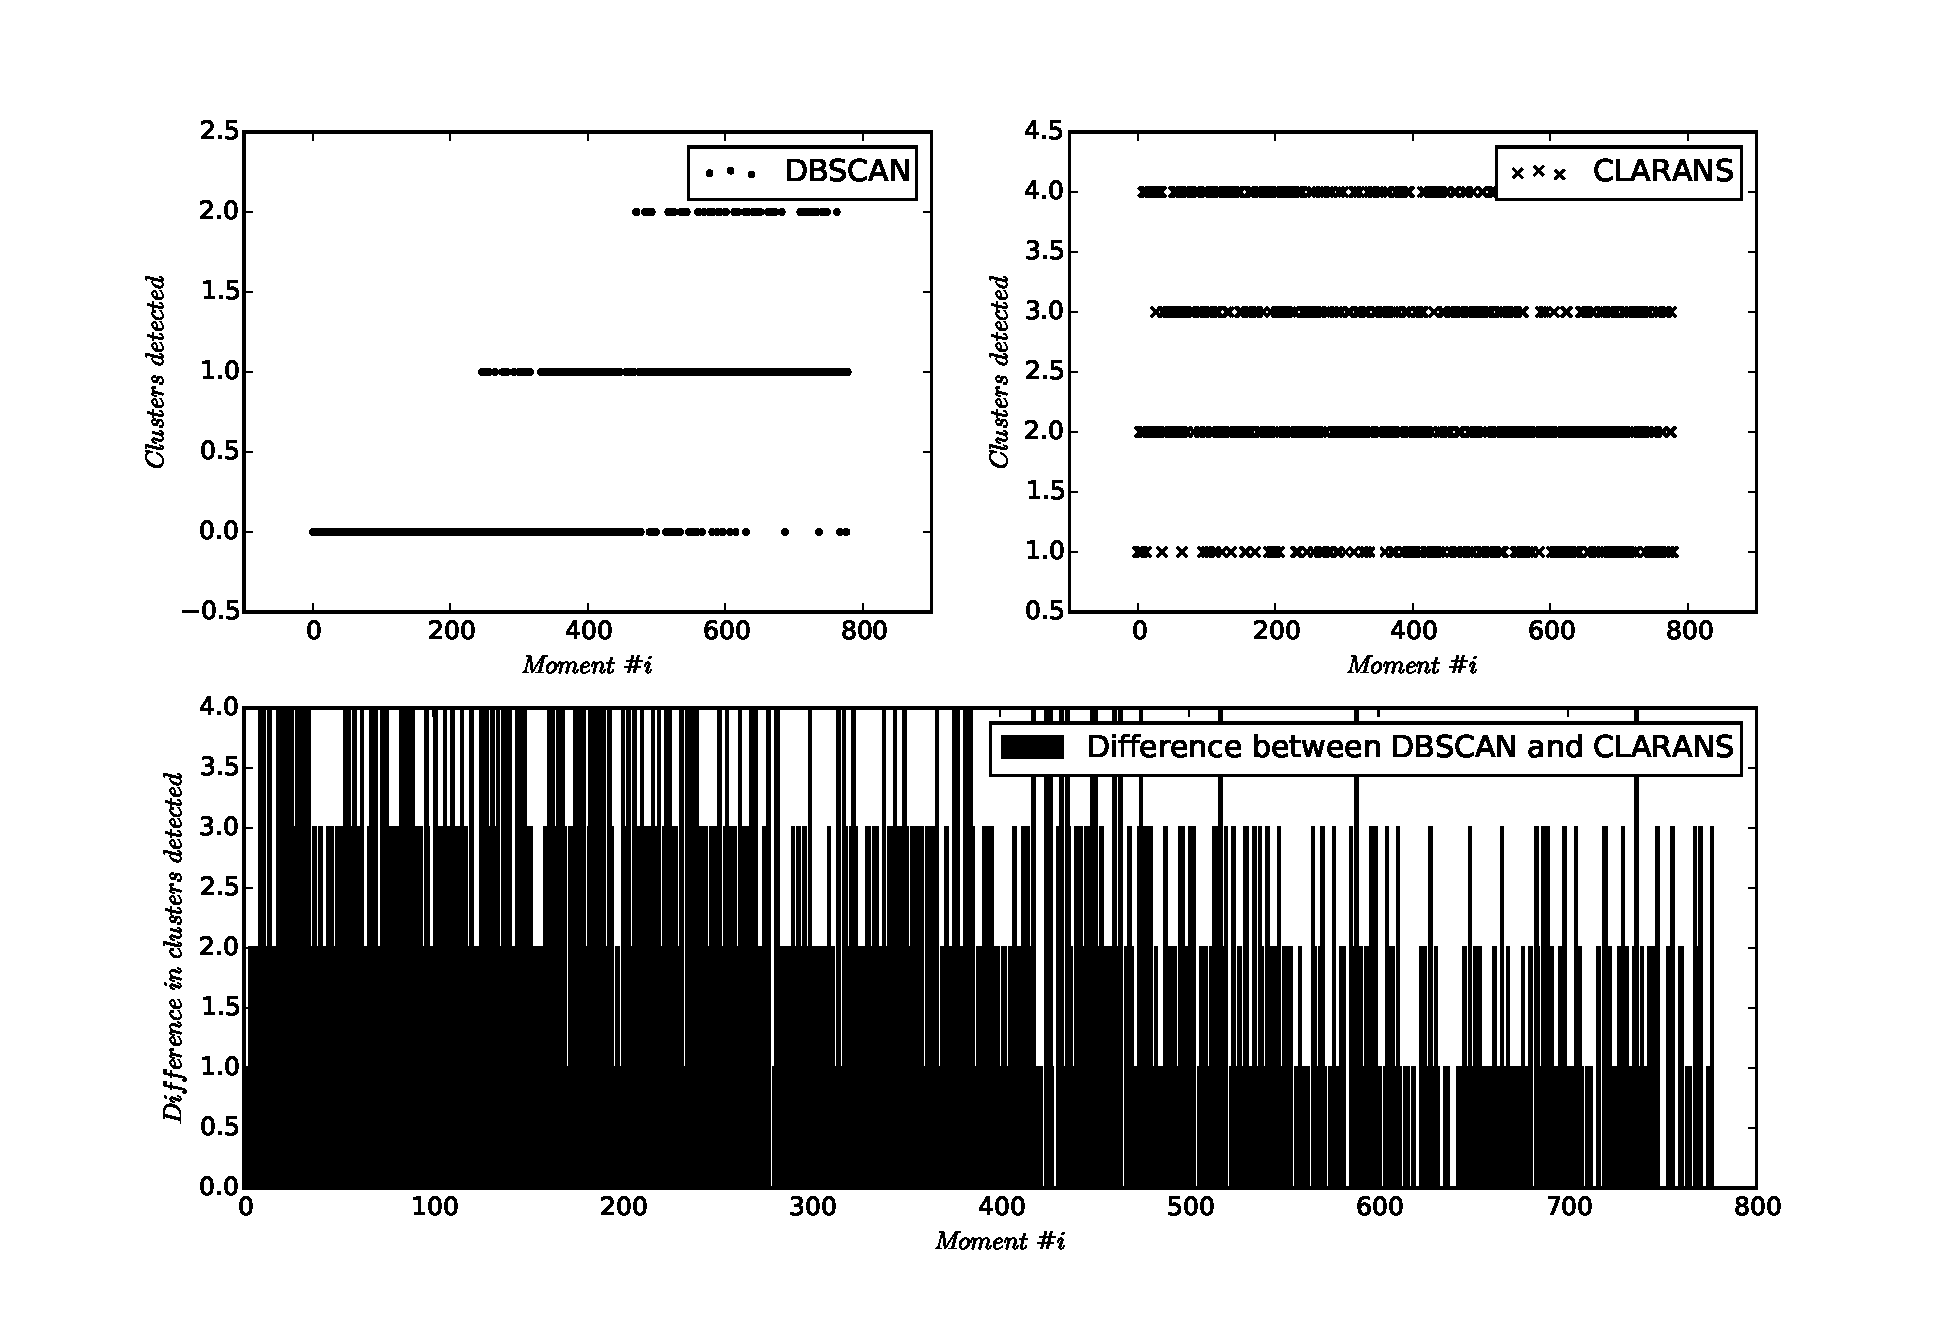
\includegraphics[width=0.9\textwidth]{plots/dbscan_vs_clarans.pdf}
    \repeatcaption{fig:dbscan-vs-clarans}
    {Cluster detection, comparison between DBSCAN and CLARANS. }
\end{sidewaysfigure}

\begin{sidewaysfigure}
    \centering
    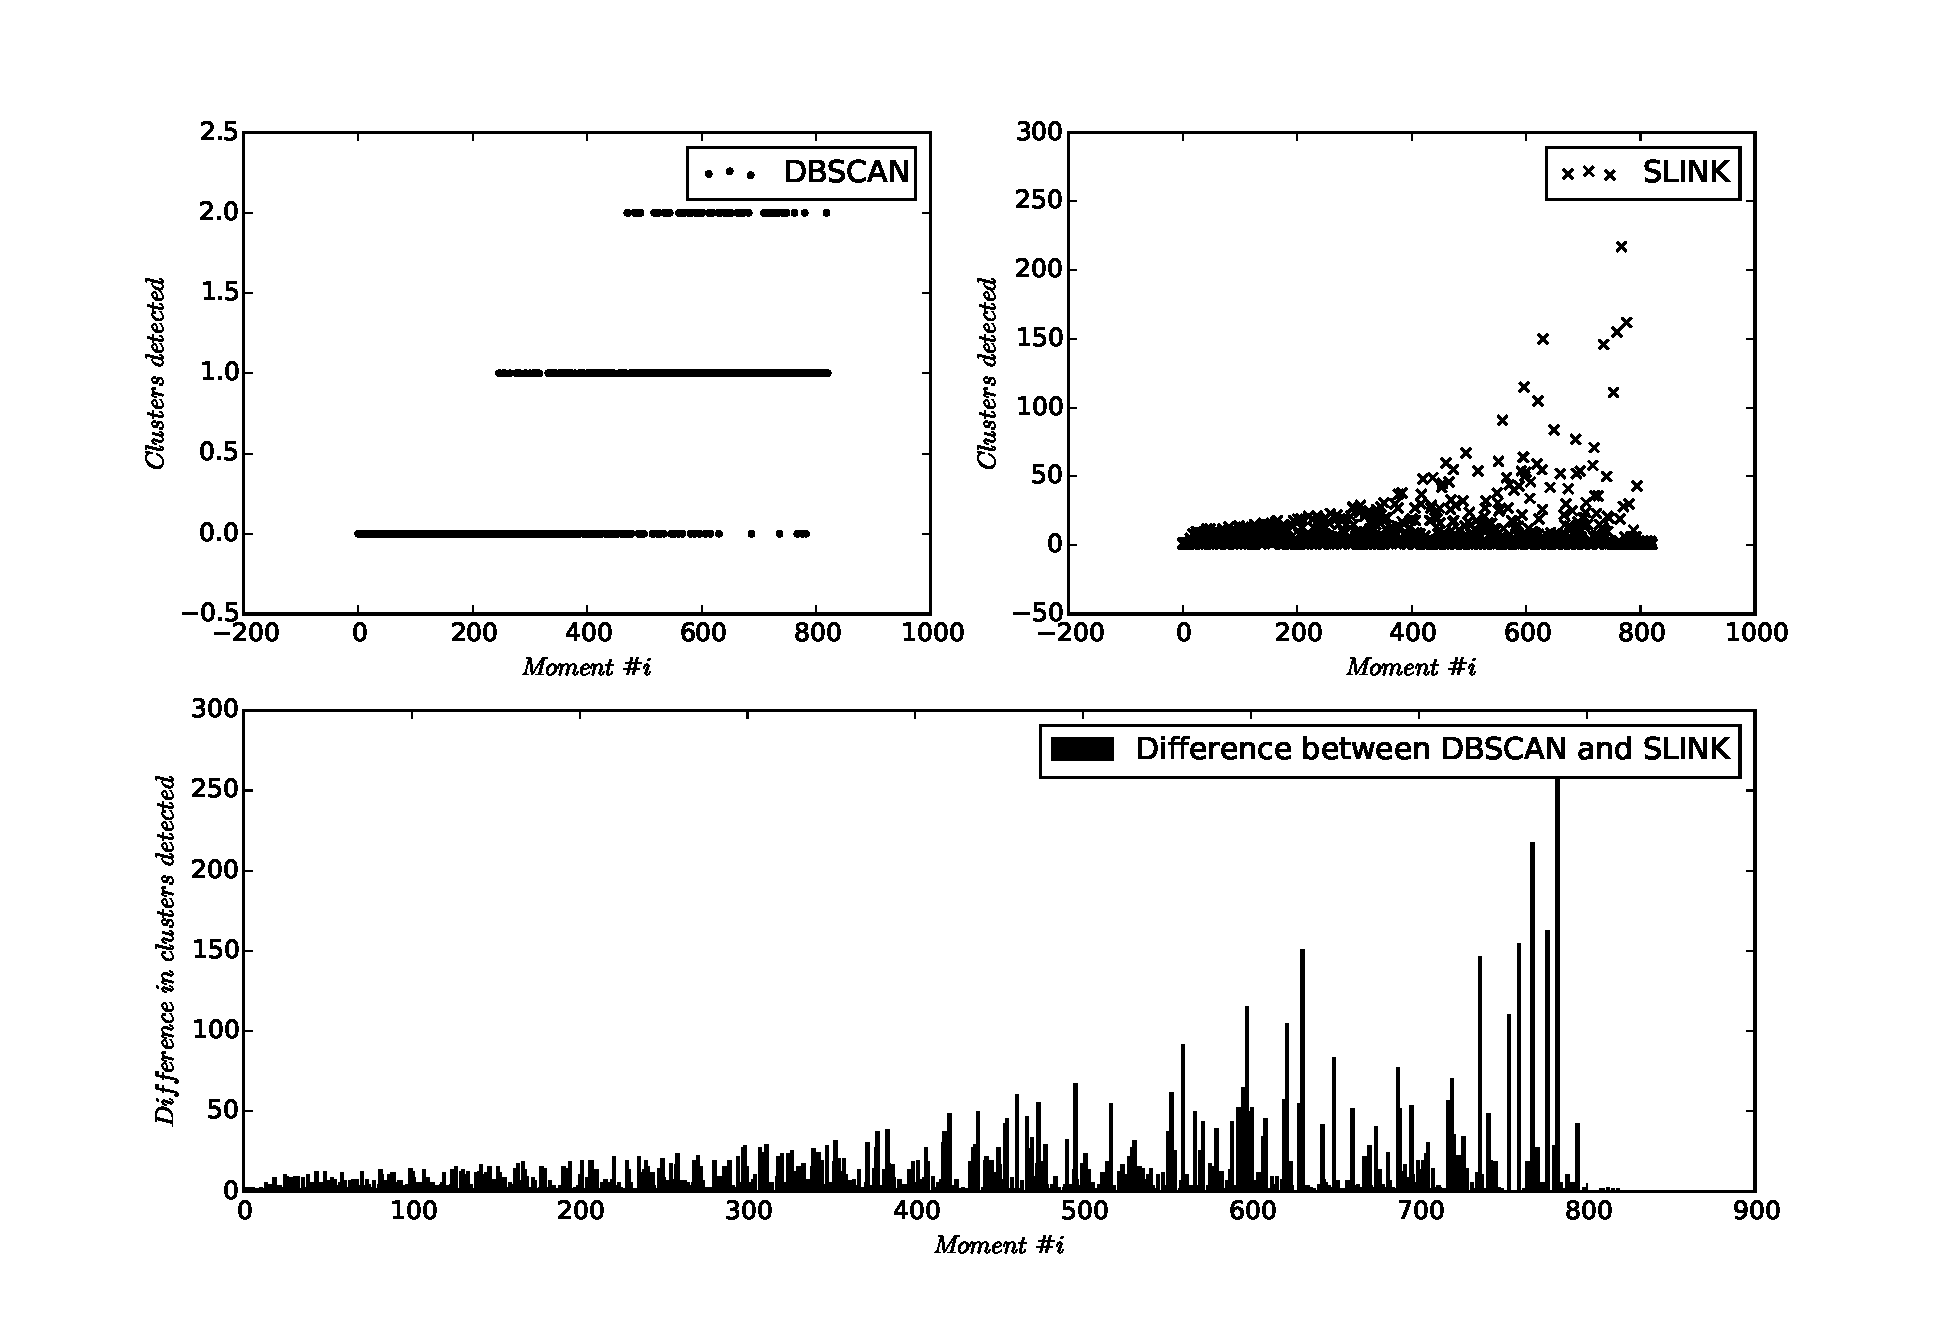
\includegraphics[width=0.9\textwidth]{plots/dbscan_vs_slink.pdf}
    \repeatcaption{fig:dbscan-vs-slink}
    {Cluster detection, comparison between DBSCAN and SLINK. }
\end{sidewaysfigure}

\begin{sidewaysfigure}
    \centering
    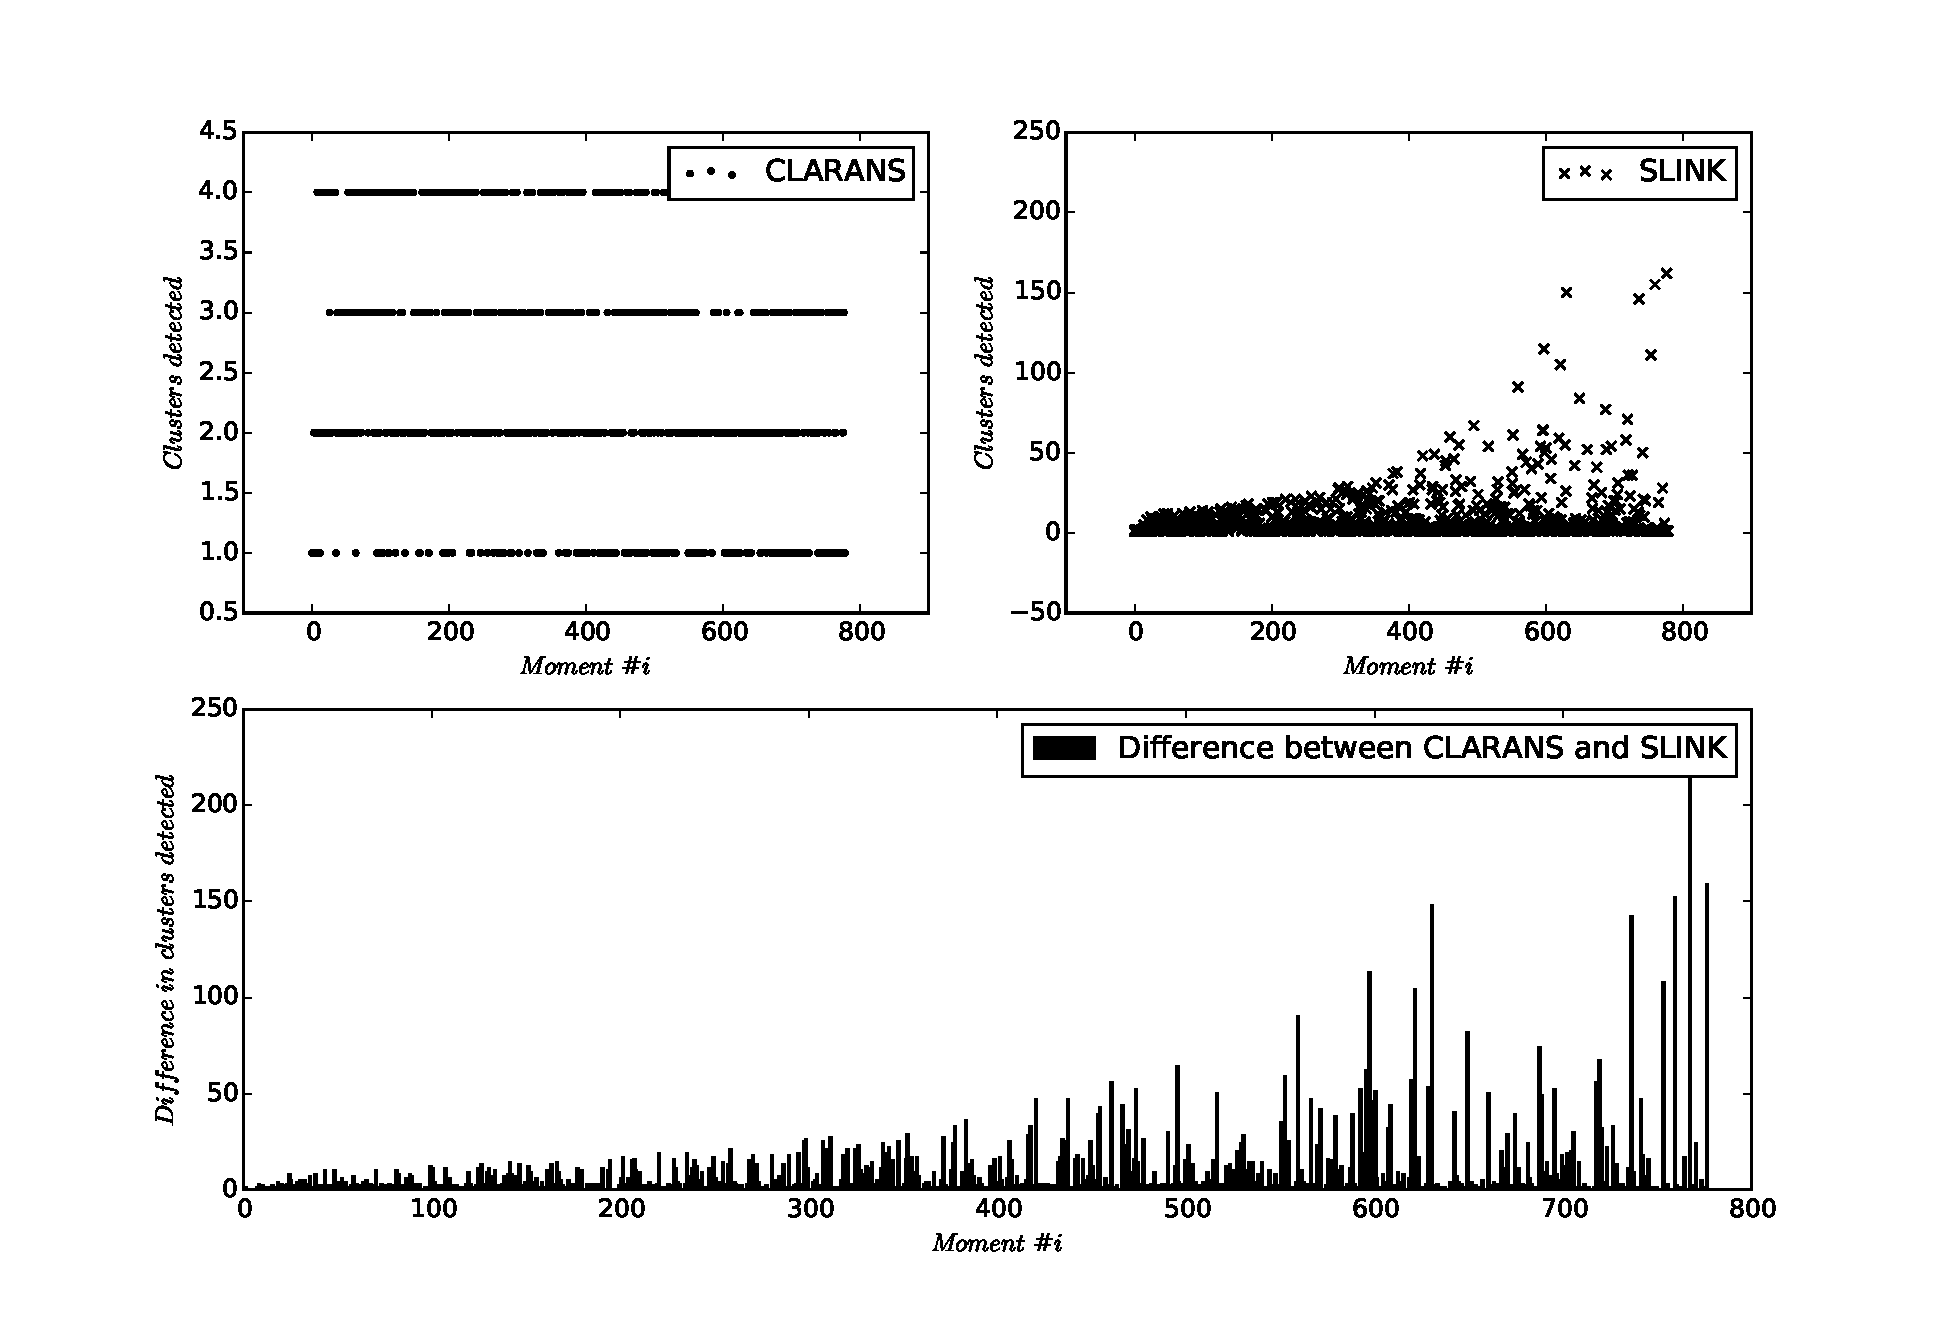
\includegraphics[width=0.9\textwidth]{plots/clarans_vs_slink.pdf}
    \repeatcaption{fig:clarans-vs-slink}
    {Cluster detection, comparison between CLARANS and SLINK. }
\end{sidewaysfigure}

\begin{sidewaysfigure}
    \centering
    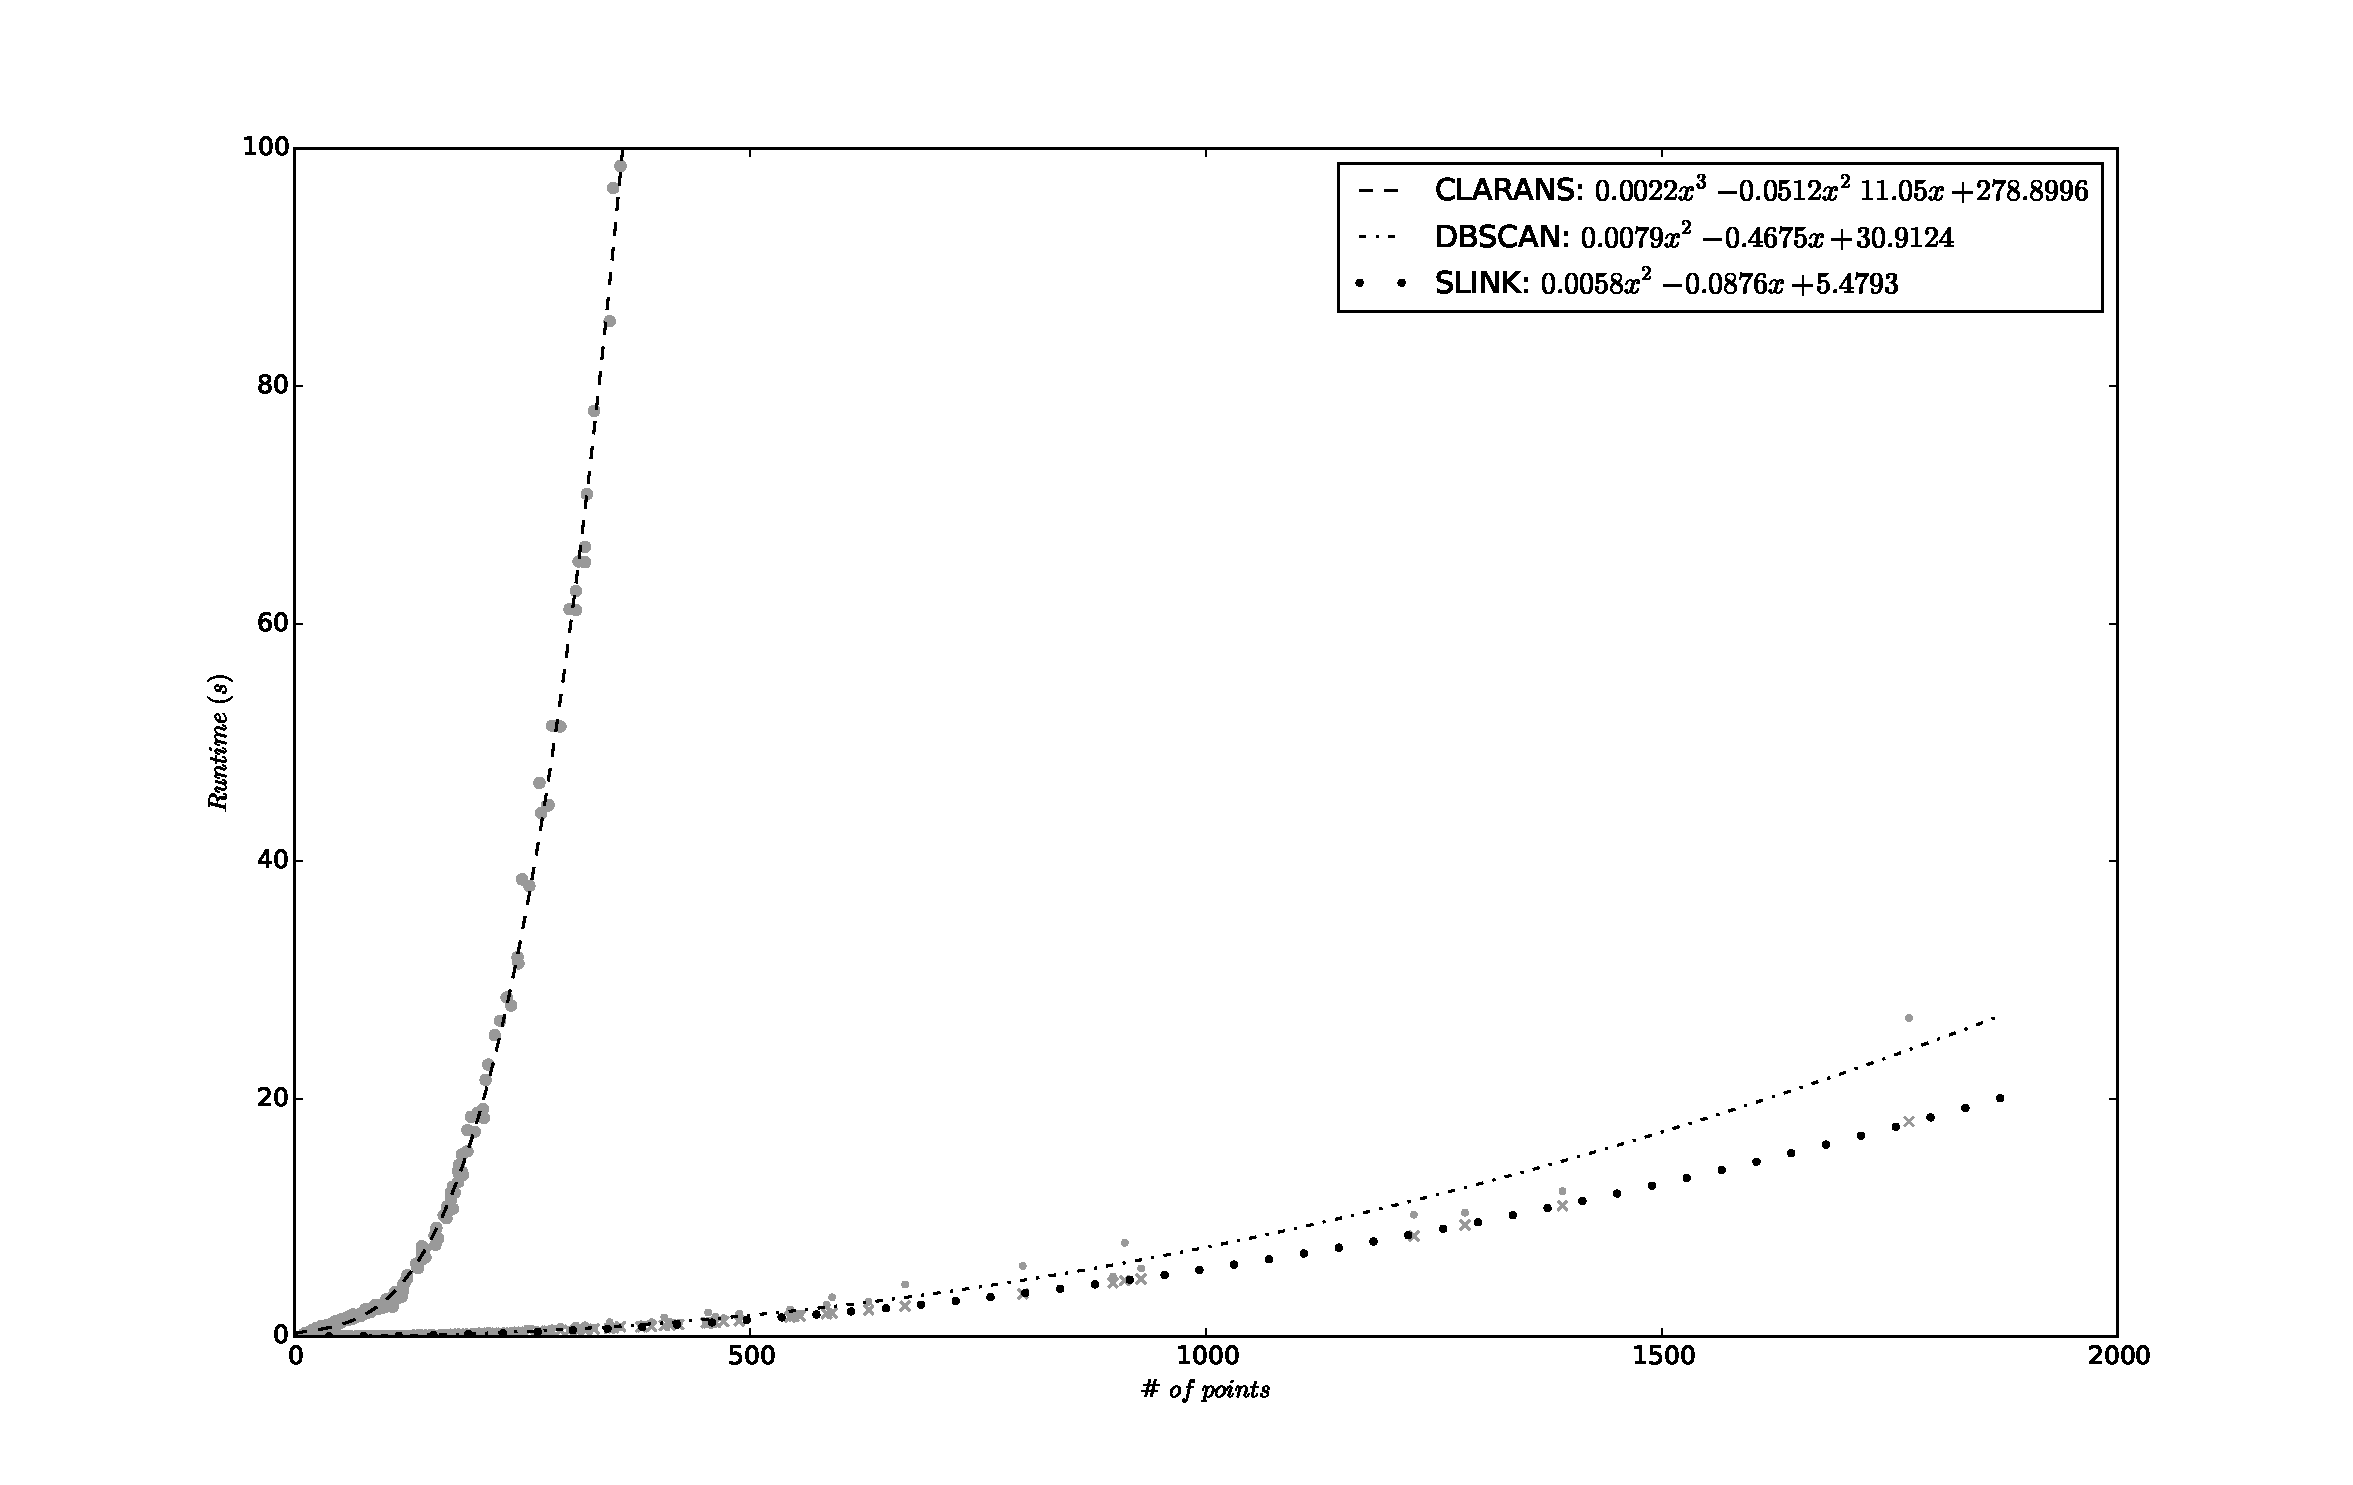
\includegraphics[width=0.9\textwidth]{plots/time_trendlines.pdf}
    \repeatcaption{fig:time-trendlines}{Scatterplot of timestamps including trend lines.}
\end{sidewaysfigure}

\end{appendices}
\addtocontents{toc}{\setcounter{tocdepth}{3}}

\end{document}
